% This document provides the style to be used for a MSc Thesis at the
% Parallel and Distributed Systems group
\documentclass[11pt,twoside,a4paper,openright]{report}

% use babel for proper hyphenation
%removed ducth babel language, I won't be using dutch anyway
\usepackage[english]{babel}
% Graphics: like the DUT logo on the front cover
\usepackage{graphicx}
% FONT: times
\usepackage{times}
% for url's use "\url{http://www.google.com/}"
\usepackage[hyphens]{url}

% for fancy header on table
\usepackage[table,xcdraw]{xcolor}

% todo notes
\usepackage{todonotes}

% because some of the author have accented name
\usepackage[utf8]{inputenc}

% use natbib to cite author easily. Change latex8 into ieee in style
\usepackage[square,numbers]{natbib}

% we love bookmarks in pdf
\usepackage[hidelinks]{hyperref}

\usepackage{caption}

\usepackage{subcaption}

\usepackage{algorithmicx}
\usepackage{algorithm}
\usepackage{algpseudocode}

% Command to abbrv the common words (I'm lazy)
\newcommand{\bt}{BitTorrent}

\begin{document}

%%%%%%%%%%%%%%%%%%%%%%%%%%%%%%%%%%%%%%%%%%%%%%%%%%%%%%%%%%%%%%%%%%%%%%%%%%%%%%%
\hoffset=1.63cm
\oddsidemargin=0in
\evensidemargin=0in
\textwidth=5in

%%%%%%%%%%%%%%%%%%%%%%%%%%%%%%%%%%%%%%%%%%%%%%%%%%%%%%%%%%%%%%%%%%%%%%%%%%%%%%%
\parindent=1em

\pagestyle{empty}

% FRONTCOVER
\begin{titlepage}

\null\vfill

\begin{center}
\LARGE{Credits in BitTorrent: designing prospecting and investments functions}
\end{center}

\vspace{1.5cm}

\begin{center}
Ardhi Putra Pratama Hartono
\end{center}

\vfill

\begin{figure}[!b]
\centering

\includegraphics[width={0.5\textwidth}]{pics/TUDlogocolor}
\end{figure}
\vspace{2.0cm}

\end{titlepage}



% EMPTY PAGE
\cleardoublepage

\pagestyle{plain}

% TITLE PAGE: page i (hidden)
\begin{titlepage}

  \begin{center}
  \null\vfill
    \begin{center}
    \LARGE{Credits in BitTorrent: designing prospecting and investment functions}
    \end{center}

    \vspace{3cm}

    \begin{large}
    Master's Thesis in Computer Science
    \end{large}

    \vspace{1.5cm}

    \begin{normalsize}
    Parallel and Distributed Systems group\\
    Faculty of Electrical Engineering, Mathematics, and Computer Science\\
    Delft University of Technology
    \end{normalsize}

    \vspace{2.0cm}

    \begin{normalsize}
    Ardhi Putra Pratama Hartono
    \end{normalsize}

    \vspace{1.0cm}

    % <MM> DD, YYYY
    \today            %TODO: Dit is de datum van uitgifte van final versie aan de afstudeer commissie

  \vfill
  \end{center}

\end{titlepage}



% GRADUATION DATA AND ABSTRACT: pages ii and iii (hidden)
%De aankondiging bevat de spreker, titel, plaats, datum en tijd, samenstelling van de afstudeercommissie en een korte samenvatting (maximaal 25 regels).
\thispagestyle{empty}

\noindent \textbf{Author}\\
\begin{tabular}{l}
Ardhi Putra Pratama Hartono\\
\\
\end{tabular}\\
\noindent \textbf{Title}\\
\begin{tabular}{l}
TODO TITLE\\
\\
\end{tabular}\\
\noindent \textbf{MSc presentation}\\
\begin{tabular}{l}
% <MM> DD, YYYY (like \today)
TODO GRADUATION DATE\\
\\
\end{tabular}

\vspace{1.1cm}

\noindent \textbf{Graduation Committee}\\
\begin{tabular}{ll}
TODO GRADUATION COMMITTEE & Delft University of Technology \\
% The order of listing the names: Graduation prof, supervisor(s), others ordered by title + alphabetical
%examples:
%prof. dr. ir. H. J. Sips (chair) & Delft University of Technology \\
%ir. dr. D. H. J. Epema           & Delft University of Technology \\
\end{tabular}

\begin{abstract} %de abstract bevat alleen een korte samenvatting van de inhoud van het onderzoek
TODO ABSTRACT
\end{abstract}

\clearpage



\pagenumbering{roman}
\setcounter{page}{4}

% EMPTY PAGE: page iv
\cleardoublepage

% OPTIONAL QUOTATION: page v
%\pagestyle{empty}

\null\vfill

\begin{center}
\emph{``TODO QUOTE''} -- TODO QUOTED PERSON
\end{center}

\vspace{10cm}

\clearpage


% EMPTY PAGE: page vi
%\cleardoublepage

% PREFACE: page v
\chapter*{Preface}
\addcontentsline{toc}{chapter}{Preface}
\vspace{1\baselineskip}

\noindent
I praise to The Almighty God for all of His countless blessing and protection.\\

This thesis is the finish line of my work as an MSc student in Delft University of Technology. Firstly, I would like to express my gratitude to my supervisor, Johan Pouwelse for pushing me and providing feedback on my work. Your excitement and enthusiasm is truly contagious. Secondly, I would like to gratefully acknowledge Endowment Fund for Education / Lembaga Pengelola Dana Pendidikan (LPDP) for giving me an opportunity to purse my master's degree. I will do my best to give back everything to my lovely country. Next, I would like to thank everyone in the 7th floor, Elric, Martijn, and Ma for supporting my work. You guys made my time in doing this work more enjoyable. 

Special thanks go to my beloved wife, Hilda Zaikarina. Your wonderful support and patience lead me to the point where I need to \textit{istiqomah} for all the work I have done. 

Last but not least, I would like to thank my family and friends for their support and motivation throughout not only my thesis, but also my study in The Netherlands. 

\vspace{1\baselineskip}

\noindent
Ardhi Putra Pratama Hartono

\vspace{1\baselineskip}

\noindent
Delft, The Netherlands

\noindent
\today

% EMPTY PAGE: page vi
\cleardoublepage

% TABLE OF CONTENTS: starting at page vii
\tableofcontents

\cleardoublepage

\pagenumbering{arabic}
\setcounter{page}{1}

% INTRODUCTION: page 1
\chapter{Introduction}
\label{chp:introduction}


%in bittorrent -> peer as social user
%
% the performance of file-sharing in p2p system
% cooperation important to keep swarm alive -> swarm evolution
%
%private trackers sometime force user to donating with SRE -> cite Chen, 2014
%this resulting poor download motivation for users although its for greater goods
%
%in the other hand, public tracker have much less SLR compared to private (has its own problem)
%
% cms do here
%
%tribler user -> many -> donate -> swarm 

Interaction among user in the Internet community can be expressed in various fashion. Peer-to-peer (P2P) is one of the major interaction existed in the net\todo{p2p owned the internet}. Many applications and protocols run on top of P2P system, online gaming, computing, and the most popular one, file sharing. \bt~is by far the most popular system used in file-sharing community with it's unique \textit{tit-for-tat} mechanism to discourage freeriding \cite{2003:bittorrent:cohen}. 

In higher abstraction level, it is common to see P2P system, specifically in \bt, as social networking. Many social challenges addressed in this kind of network such as incentives mechanism, economical value to survive in the community, reputation identification, and user anonymity\todo{cite here and there about those study}. All of those challenges involves peer behavior whether to help each other for the greater goods, selfishly consume all the resource without giving back, or inconsistently act between these two. Based on \todo{cite, peer behavior}, lots of P2P peers are always show self-interest and rationality. It can be interpreted as maximizing their benefits and giving as little as possible. \textit{Freeriding} is the term given to this kind of behavior. It is often to describe this peer as \textit{freeriders}.

In \bt~system, cooperation between peers is very important to keep a file available in the network. With more user provides the file, the download speed gained for other user will be increased as well. However, this needs user enthusiasm for providing the file regardless of its needs. For both public and private communities, the number of seeder become an issue that made a swarm unhealthy \cite{2010:pubpriv:meulpolder, 2014:sustainabilitytorrent:chen}. With freeriders join the swarm, naturally it will reduce the overall performance. Furthermore, when freeriders become majority, the swarm is as good as dead \todo{cite this, I read this somewhere}. 

%example of solution
% This problem is commonly addressed as prisoner's dilemma \todo{prisoner dilemma citation}.
Several researches already provide solution to prevent uncooperative peer behavior\todo{cite here and there}, all to produce higher downloading throughput on downloader. Most of them focused their work on the incentives for peer or alteration of the currency system itself. Tribler for example, working on a MultiChain \cite{2015:multichain:norberhuis} as a secure and accountable currency in P2P system. \todo{another client address freeriding, incentive, etc} This thesis work is more general and applicable as an another spectrum hoping to solve this problem. 

%what this thesis do
%credit mining tries to solve, 
%design, implement, evaluate. also with normal downloading
In this thesis, we introduce ``Credit mining system (CMS)'', an automatic investment framework on swarm with multidimensional gain. The first phase of the framework was conducted by \citeauthor{2015:creditmining:capota}, mainly to operate CMS without any restriction or coordination with any client. With CMS, locally, a user can gain credit with internal limited bandwidth allocation without any intervention needed. The credit can be in many forms such as share ratio (upload-to-download ratio), uploaded amount, effort based credit, and many other. From higher perpective, CMS will help a swarm to keep alive by providing integral pieces to peer who need it. Although CMS will be implemented in Tribler system, it is possible to implement this feature to any system on top of \bt~ network.

Tribler is one of the P2P file sharing software developed in Delft University of Technology that addressing social issues in \bt~network\cite{2008:tribler:pouwelse}. With Tribler downloaded from official repository on the latest stable release (6.5.2) reaching  78440\footnote{\url{http://www.somsubhra.com/github-release-stats/ ?username=tribler&repository=tribler} (Accessed 3 September 2016)} times, it is desired to observe the usage of CMS with adequate user base. We believe our work will be able to increase the overall swarm throughput by donating unused bandwidth on peer upstream.


%
Credit (share ratio or upload rate) is needed especially in private tracker. In this case, BitTorrent tit-for-tat is irrelevant \cite{2010:pubpriv:meulpolder}




\section{Peer-to-peer networks}
In this section we will discuss several aspects of peer-to-peer (P2P) networks. \todo{Structure of this section}



P2p in social aspect
freeriding
prisoner dilemma -> reduce througput

private tracker/community solve lack of initiative -> incentivize

different p2p app (file transfer, vod, game), have different requirement

flashcrowd -> sudden increase in net -> unstable peer. supply demand misalignments -> non heavy tail

% some to increase throughput
smart cloud seeding -> mix download from cloud and p2p. Analysis on which swarm/file to help

% problem: p2p social community is good if all peer is considerable, otherwise, it sucks.bittorrent pattern flashcrowd : many S/L, only at the beginning.  deteriorate afterwards. User rewarded for providing old content?

% probably not
reputation, credit


\section{Economics in distributed system}
Demand and supply \cite{2009:demandsupplyres:andrade}\\

Public tracker generally slow\todo{find citation}. Why? 

private > public
oversupply, undersupply -> not all necessary to be mined \cite{2015:sustainabilitypt:vinko}
investment in swarm (decision)
motivation in priv and public

incentive -> various, centralized, decentralized. Complicated or not. modifying bittorrent protocol? -> not standard 

\section{Optimizing network cost}
Anonymous Relaying performance in Tribler \cite{2015:onionroutetribler:stokkink}\\
Significant portion when seeding million torrents \cite{2012:milliontorrent:arvid}

\section{Main Contributions}

\subsection{Research Questions}

\section{Document Structure}
This thesis is structured as follows. Chapter 2 discusses related work to the problem and solution proposed. Chapter 3 presents the design of credit mining system integrated with Tribler. Implementation of the mechanism and it's experiment will be elaborated in chapter 4. Chapter 5 shows performance of credit mining system. At the end, chapter 6 concludes the work mentioning possible future work.


% CHAPTERS
\chapter{Problem Description}
\label{chp:relwork}
In this thesis, we introduce ``Credit mining system'', an automatic investment framework on swarm with multidimensional gain. The prototype of the framework was conducted by \citeauthor{2015:creditmining:capota}, mainly to run credit mining system without any restriction or coordination with any client. With credit mining system, locally, a user can gain credit with internally limited bandwidth allocation without any intervention needed. The credit can be in many forms such as share ratio (upload-to-download ratio), uploaded amount, effort based credit, and many other. From higher perspective, credit mining system will help a swarm to keep alive by providing integral pieces to the peer who need it. Although credit mining system will be implemented in Tribler system, it is possible to apply this feature to any file-sharing system.

\todo{3 problem - 1 prior work - 2 question}
In this chapter, three problems that are the main concern of this thesis will be elaborated. First we will discuss cooperation and performance problem in peer-to-peer system, specifically \bt. The characteristics and importance of cooperation in peer-to-peer network \bt~will be reviewed. Secondly, the issue of \bt~credit and investment will be explained as the main concern of this work. It covers the importance, potential gaining, and desired effect of the possible credit investment. Thirdly, we will illustrate how much the bandwidth resource might be consumed by crawling in \bt~ecosystem. After specifying problems, prior works on credit mining will be reviewed. Further improvements on those work are the core of this thesis. Lastly, two research questions will be formulated.

\section{Cooperation and performance in \bt}

% social in p2p
In higher abstraction level, it is common to see P2P system, specifically in \bt, as social networking. Many social challenges, such as incentives mechanism, economic value to survive in the community, reputation identification, and user anonymity, addressed in this kind of network. All of those challenges involves peer behavior whether to help each other for the greater goods, selfishly consume all the resource without giving back, or inconsistently act between these two. It can be interpreted as maximizing their benefits and giving as little as possible. \textit{Freeriding} is the term given to this kind of behavior. It is often to describe this peer as \textit{freeriders}. Based on study by \citeauthor{2000:freeridegnutella:adar}, lots of P2P peers are always show self-interest and rationality, that is, freeriding \cite{2000:freeridegnutella:adar}. In Gnutella case, it even reaches 70\% of its user.  However, \citeauthor{2005:bittorrentcooperation:andrade} showed that \bt~is indeed increased cooperation with only less than 10\% peer is uploading something. In \textit{private community}, this has gone better with higher SLR \cite{2005:bittorrentcooperation:andrade}. Even \citeauthor{2015:freeriderinbtcommunity:das} found that freerider in \bt~ does not deteriorate system performance\cite{2015:freeriderinbtcommunity:das}. All of this fact, however, does not change the fact that P2P users generally are still selfish \cite{2014:userbehaviourprivate:jia}. 

% cooperation is important in bt
In a \bt~system, cooperation between peers is crucial to keep a file available in the network. With more user provides the file, the download speed gained for other users will be increased as well. However, this needs user enthusiasm for providing the file regardless of its needs. For both public and private communities, the number of seeders becomes an issue that made a swarm unhealthy \cite{2010:pubpriv:meulpolder, 2014:sustainabilitytorrent:chen}. With freeriders join the swarm, naturally, it will reduce the overall performance. Furthermore, when freeriders become a majority, the swarm is as good as dead \cite{2000:freeridegnutella:adar}. 

% public vs private community. compare performance
\bt~ community can be divided into two categories : \textit{public} and \textit{private}. A community usually served by a \textit{tracker}. Public tracker means everybody can join the swarm served by that tracker. In the other hand, private communities are closed community which can be accessed by passing particular requirement \cite{2010:pubpriv:meulpolder, 2014:sustainabilitytorrent:chen}. \citeauthor{2010:pubpriv:meulpolder} measured that private communities have 3-5 times higher download speed compared to public communities \cite{2010:pubpriv:meulpolder}. This benefit makes joining private community is typically harder compared to public community.

% issue in both community. Imbalance.
Despite has different performance, both public and private community suffer from a similar issue: ``Poor downloading experience''. It is widely known that public community generally has low SLR which directly affect the swarm performance. In the other hand, private tracker suffers from ``\textit{poor downloading motivation}'' as described by \citeauthor{2014:sustainabilitytorrent:chen}\cite{2014:sustainabilitytorrent:chen} although private community intended to solve low SLR issue. The poor downloading motivation on private tracker affect the sustainability of a swarm. The imbalance of demand and supply will harm new members of private community and gradually degrade the motivation to keep active in the community for another user \cite{2014:sustainabilitytorrent:chen}.

% the necessity to add more reputation management using cooperation. To monetize cooperation.
Peer-to-peer file sharing community, especially \bt~ can improve the user downloading experience. It does not give strain to server connection and naturally will download as fast as possible depending on file availability. However, uncooperative peer behavior and low file availability can affect a swarm's health thus reducing download experience. To complement tit-for-tat mechanism, it is necessary to implement global incentive scheme in \bt. Some researchers start by leveraging the reputation system for peers. This also supported by \citeauthor{2002:reputationtotragedy:milinski} that reputation can help solving ``tragedy of the commons'' problem \cite{2002:reputationtotragedy:milinski}. The mechanism can be centralized on decentralized. Private communities that enforce SRE is an example of centralized mechanism. The reputation of user is stored in the server while it update the data in the communication via tracker. BarterCast \cite{2009:bartercast:meulpolder} and its successor MultiChain \cite{2015:multichain:norberhuis} are the example of decentralized incentive mechanism that works on top of reputation system. 

%Several kinds of researches already provide solutions to prevent uncooperative peer behavior, all to indirectly push higher downloading throughput on downloader.
%Most of them focused their work on the incentives for peer or alteration of the currency system itself. Tribler for example, working on a MultiChain \cite{2015:multichain:norberhuis} as a secure and accountable currency in P2P system. \citeauthor{2008:givetogetvod:Mol} published free-riding resilient algorithm for Video on Demand (VoD) in P2P environment\cite{2008:givetogetvod:Mol}. \citeauthor{2015:incentivep2pgame:kang} used game theory as a formulation to incentivize peer in order to prevent free-riding behaviour\cite{2015:incentivep2pgame:kang}. They also considered mobile P2P network which only capable of low complexity mechanism. In their work, peers are awarded with different credit depend on connection type and content.
% problem: p2p social community is good if all peer is considerable, otherwise, it sucks.bittorrent pattern flashcrowd : many S/L, only at the beginning.  deteriorate afterwards. User rewarded for providing old content?

\section{The confusion in \bt~credit investment}
In peer-to-peer system, specifically in \bt~protocol, \textit{incentive mechanism} is introduced to tackle freeriding problem \cite{2003:bittorrent:cohen}. With limited resource possessed by each peer, there is a price that need to be paid on accessing resource. The whole collection of transaction created incentive system which should be defined in order to extract user goodness in computational way.

In economic terminology, it is necessary to specify a value of the resource that can lead to the ``wealth'' of a user. In \bt~system ``credit'' can be defined in various object. For specific, private community such as DIME\footnote{\url{www.dimeadozen.org}}, \citeauthor{2012:economicbt:kash}  defined credit as \texttt{4 x upload - download} in bytes, accumulated for all the torrent served in that community \cite{2012:economicbt:kash}. \citeauthor{2015:creditmining:capota} assume the credit on his work as the difference between uploaded and downloaded bytes. \citeauthor{2014:sustainabilitytorrent:chen} mentioned another form of credit that can be earned depend on the activity, for example, seeding more torrents, seeding longer and old torrent, and seeding torrent that consumes large disk space\cite{2014:sustainabilitytorrent:chen}. In \bt, incentive system is enforced by its choking algorithm. It prefers to give the resource to the one who has the highest credit, in this case, the upload rate. In general file-sharing peer-to-peer application, user will receive credit when they upload data to others.

With credit as a token of incentive, user can ``spend'' the credit to get service from someone else. In many communities, this means that user can download more files. It is also possible that this credit may be spent to get other facilities in the community such as right to access specific content, get higher download speed, and receive social acknowledgement. Naturally, having many credit as user disposal may be advantageous \cite{2014:sustainabilitytorrent:chen}. At the point user aware of this achievement, he may want to \textit{invest} his already owned credit to get more credit.

Although high credit for user is desirable, one must be aware the effect of overwhelming credit on few users is bad for the community. Therefore, it is important to balance credit mining and community overall performance. \citeauthor{2015:sustainabilitypt:vinko} showed that both of them have conflicting interest. High few individual performance can lead to lower overall community performance \cite{2015:sustainabilitypt:vinko}. Moreover, \citeauthor{2013:survivepriv:jia} also mentioned that oversupply swarm because of overwhelming seeders may result in lower bandwidth allocation for other users \cite{2013:survivepriv:jia}. Not to mention undersupply problem that common in public community which gives very poor performance.

We define the activity of downloading with the expectation of obtaining credit to use later on as \textit{investment}. The act of seeding to help to increase the community performance graciously is called \textit{donating}. A user can \textit{prospect} which community he will invest or donate regardless of his own resource. Not all the swarm need to be seeded as we shown the drawbacks of oversupply. The prospecting and identifying swarm that needs to be seeded based on the seeder's intention (whether to invest or donate) is important. By providing proper prospecting function, users could help each other to improve the swarm quality. In good investing algorithm, users can make better use of its resource to gain credits when prospecting a swarm. 

To the best of our knowledge, there are very few works addressed credit investment in \bt. \citeauthor{2013:survivepriv:jia} mentioned how inefficient the practice of seeding for a long time to get credits. Ironically, the long time seeding is commonly practiced as it is the most trivial way to maintain credits \cite{2013:survivepriv:jia}. Three prior work has been done by \citeauthor{2015:creditmining:capota} \cite{2015:creditmining:capota, 2013:investmentcm:capota, 2014:bwmarket:capota}. This will be discussed in section \ref{section:cmprior}. 

\subsection{Gain return and performance by spending credit}
% Distinction invest vs donate.
The activity of spending credit can be categorized as three : (i) \textit{trading}, (ii) \textit{investing}, and (iii) \textit{gifting} or \textit{donating}. When a user want to spend his credit to get something, we define it as \textit{trading} or buying. This is most common case, because in credit-based community, every content has its price. \textit{Gifting} is the case when a peer consciously intend to not getting any direct, immediate, or obvious return of his credits \cite{2006:gifting:ripeanu}. The purpose of this action is usually to improve the performance of a community. Gifting can also act as a reward because a peer is satisfied with the community. Investment is the activity of spending credit with the expectation of obtaining credit to use later on. 

% helping others in p2p, improve performance
Recent work on helping other user to increase downloading performance using \bt~ has been done. \citeauthor{2014:cloudseed:leon} uses \bt~ protocol to increase user download speed and at the same time reduce datacenters load. They analyze which swarm or file to help using user bandwidth information and number of connected user\cite{2014:cloudseed:leon}. From another perspective, \citeauthor{2015:coalitionbt:zhang} introduced the \textit{coalition} between \bt~ peers. Coalition is a set of peers that cooperate each other in regards to \bt~policy to minimize download completion time. They also propose coalition-compatible choking strategy to replace the current \bt~one. This research lead to significant performance improvement within the coalition \cite{2015:coalitionbt:zhang}. Although not using \bt~protocol, in \citeyear{2009:p2phelp:he}, \citeauthor{2009:p2phelp:he} proved that helper peer also can improve the streaming capacity in P2P system\cite{2009:p2phelp:he}. \citeauthor{2016:gameauctionp2pstream:mostafavi} extend this work by introducing auction aspect for uploader to choose which user will receive the bandwidth he donate \cite{2016:gameauctionp2pstream:mostafavi}. \citeauthor{2016:gameauctionp2pstream:mostafavi} used game-theory to propose new framework in uncooperative peers with maximizing the credit gain for helpers.

% the importance of healthy swarm -> public good, prevent tragedy of the common. user is selfish, it is good to donate. Reality : they want something in return -> credit. Move the problem into investment problem. 
The ideal situation of balanced high performance and sustainability in \bt~community is desired by align supply and demand as discussed in section \ref{section:suppdemand}. By gifting and helping undersupply community adequately, the optimal situation can be achieved and tragedy of the common can be prevented \cite{2002:reputationtotragedy:milinski}. However, commonly, that is not the case. P2P user are typically selfish in economical way \cite{2014:userbehaviourprivate:jia}. By gifting, it will take ones resource without any return. In fact, common user wanted some return as compensation. Therefore, investment is the most feasible method to balance user and community needs.

% find low price, sell high price
In classical economic principal, the key to gain benefit is to buy low and sell high. However, this property depends on the item and the market condition. If we translate it into \bt~ economic environment, the item is the file, and the condition is the swarm. \citeauthor{2012:economicbt:kash} introduced term is \textit{resale value}. Resale value is the amount of \textit{gross} credit one will get by uploading a file. In DIME case, it is 4 times uploaded bytes. In other words, resale value is the amount of return one can expect by uploading a file. We saw this mechanism as a way to incentivize user. Because by uploading one byte, a user can get 4 credit which can be used to spend/download 4 bytes. By finding popular item and suitable swarm, the potential of investment become huge.

\section{Optimizing resource}
To gain credit, seeding is necessary. However, users are forced to seed for excessively long time to maintain adequate credit \cite{2013:survivepriv:jia}. \citeauthor{2013:survivepriv:jia} also stated that this activity is commonly practiced although it is not productive. By seeding unproductively, user wastes his resources, such as bandwidth, storage capacity, and computer power.

In larger scale, if we meant to seed a lot of torrents, for example, a million, the bottleneck occurred will be more fundamental. \citeauthor{2012:milliontorrent:arvid} shows an example how costly the \textit{announce} request accompanied by \textit{response} payload can be. Seeding 1 million torrent with announce once per every hour, which is half of the default interval, need 130 kB/s upload and 75 kB/s download bandwidth constantly \cite{2012:milliontorrent:arvid}. This value is significant for most of common Internet connection.

Most researches have measured \bt~ by crawling its community pages \cite{2013:survivepriv:jia, 2005:bittorrentcooperation:andrade, 2014:userbehaviourprivate:jia, 2010:pubpriv:meulpolder, 2014:sustainabilitytorrent:chen, 2012:economicbt:kash, 2013:investmentcm:capota, 2009:demandsupplyres:andrade, 2011:interswarm:capota}. This way, they can get the data summarized by the pages. Some researches contact the tracker regularly or using its dump logs \cite{2011:yoshida:crawlbtnet, 2005:bittorrentcooperation:andrade,  2015:freeriderinbtcommunity:das, 2011:interswarm:capota}. Most of the research using logs as its dataset only use single tracker to monitor a particular torrent. Few of the research use instrumented client or directly observe the \bt~environment by understanding peer behavior \cite{2010:pubpriv:meulpolder, 2013:swarmevolution:su}. A work conducted by \citeauthor{2010:btworld:wojciechowski} discussed several method of \bt~measurement. The methods shown in table \ref{tbl:btmeasuremethod}.

\begin{table}[ht]
	\centering
	\caption{\bt~measurement techniques \cite{2010:btworld:wojciechowski}}
	\label{tbl:btmeasuremethod}
	\begin{tabular}{|l|l|l|}
		\hline
		\rowcolor[HTML]{C0C0C0} 
		\multicolumn{1}{|c|}{\cellcolor[HTML]{C0C0C0}\textbf{Level}} & \multicolumn{1}{c|}{\cellcolor[HTML]{C0C0C0}\textbf{Advantage}} & \multicolumn{1}{c|}{\cellcolor[HTML]{C0C0C0}\textbf{Disadvantage}} \\ \hline
		Internet & Excellent coverage & ISP collaboration \\ \hline
		Community & Implementation & Peer details \\ \hline
		Swarm & Details & Context \\ \hline
		Peer & Details & Scalability \\ \hline
	\end{tabular}
\end{table}

In the following section, we will focus on the measurement technique with peer discovery. With the trackless \bt evolved in early 2008 by DHT protocol \cite{2008:dht:loewenstern}, monitoring trackers may result in inaccurate result. Moreover, the credit mining mechanism heavily rely on real-time data which can not be obtained from querying the community pages.

% peer discovery DHT, PEX, LSD
\subsection{Peer Discovery}
One of the integral part in \bt~protocol is peer discovery. With numerous known peers, the algorithm will have more option on which peer to unchoke. State of the swarm itself often represented by the peer belong to that swarm. As mentioned before, it is relatively costly just to discover new peers if there are a lot of swarms monitored. 

In \bt, there are four methods to discover new or update peer. Those are using centralized trackers, distributed hash table (DHT), peer exchange (PEX), and local service discovery (LSD). The methods will be described below.

\subsubsection{Tracker Peer Announce}
In original design of \bt, it uses tracker to allow peer discover each other \cite{2003:bittorrent:cohen}. Tracker tends to use random and limited list of peers. Peer contact tracker periodically to expand their peer dictionary. This act of requesting peer to tracker is called \textit{announce}.	Usually, most tracker has a policy about recommended interval when to recontact for getting new peers. Violate this policy can result a particular peer blocked.	
	
\subsubsection{Distributed Hash Table (DHT)}
Originally, peer needs to contact tracker to fetch new peer address and file information. This makes \bt~very dependent on centralized system which vulnerable to single point of failure. In 2008, Distributed Hash Table (DHT) was proposed \cite{2008:dht:loewenstern}. Towards a ``trackerless'' \bt~system, DHT allows each peer to become a tracker. DHT stores peer contact information with defined key-space as ``node ID''. Each peer stored other peer's node ID and its address in their own routing table. A ``distance'' is measured on two node ID to define how close those two. ``Distance'' also can be measured between infohash of a torrent and node ID.
	
To enrich its peer dictionary, a node can compare a torrent's infohash and node ID in its routing table. If the distance under the threshold, it contacts that node to ask the information of the swarm, which includes the peer list. If contacted node do not know this torrent, it will respond with another node in its table which closest to the provided infohash. 
%\todo{expand_:DHT performance?}

\subsubsection{Peer Exchange (PEX)}
To increase the chance of getting higher downloading speed, having up to date peer is desired. This can be achieved by contacting tracker or using DHT. Reducing the interval of contacting tracker can result in getting a number of updated peer sooner, however, it will put a burden on the tracker itself. Peer Exchange (PEX )\cite{2015:PEX:the8472} is proposed to tackle this problem. PEX used list of peers that bootstrapped from another mechanism. This mechanism allows contacting known peer directly to get and give up-to-date information on swarm. Theoretically, it can keep this swarm together if trackers are down. Specification mentioned in \cite{2015:PEX:the8472} stated a restriction such as number of request per minute and number of peer added or removed in a PEX message.
	
\subsubsection{Local Service Directory (LSD)}
To increase the performance when downloading from a swarm, it is preferable to get the file from local network if available. Local service directory (LSD) permit this by discover peers that are in the same local network. The transfer rate is much higher compared to other type of peers. In short, LSD uses multicast-like mechanism which broadcast infohash of a torrent.
%\\
%Anonymous Relaying performance in Tribler \cite{2015:onionroutetribler:stokkink}\\
%Significant portion when seeding million torrents \cite{2012:milliontorrent:arvid}
%
%check swarm scrape -> multiple research -> based on dump logs

% piece population study -> http://ieeexplore.ieee.org/document/4410992/?arnumber=4410992
% related : Legout's work

% characteristics : http://www.sciencedirect.com/science/article/pii/S1389128610003622

\section{Prior Credit Mining Research}
\label{section:cmprior}
Preliminary work on credit mining has been done by \citeauthor{2015:creditmining:capota} \cite{2015:creditmining:capota, 2013:investmentcm:capota, 2014:bwmarket:capota}. On the prototype they made, they implement complex method with speculative download to assess the swarms\cite{2013:investmentcm:capota}. Extending this work, they introduced \textit{helper} peer to seed low capacity swarm using libtorrent \textit{share mode}\cite{2014:bwmarket:capota}. Recently, they moved into multiple swarm approach and using public community as their research object. With swarm selection policy, they observed whether helper peer can generate high credit with less downloading\cite{2015:creditmining:capota}.

\begin{figure}[ht]
	\centering
	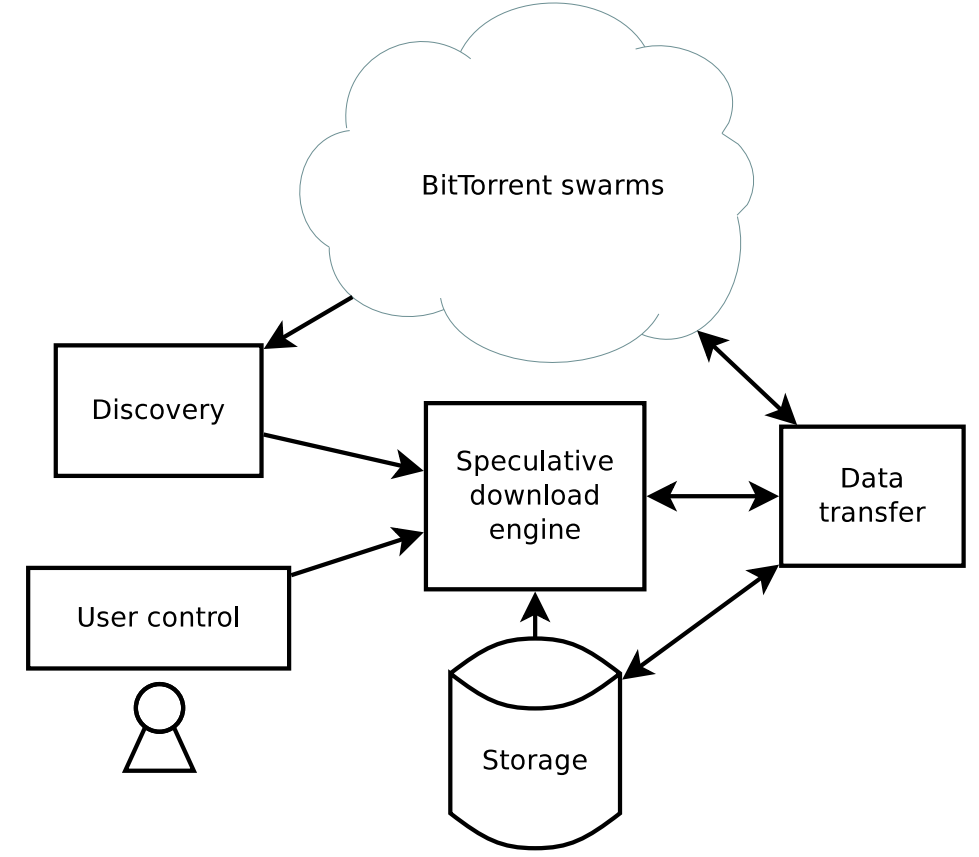
\includegraphics[width=0.7\textwidth]{pics/SDE2013.png}
	\caption{Speculative download mechanism \cite{2013:investmentcm:capota}}.
	\label{fig:sde13}
\end{figure}

In \citeyear{2013:investmentcm:capota}, \citeauthor{2013:investmentcm:capota} introduced bandwidth investing in \bt~private communities. He applied speculative download (as shown in figure \ref{fig:sde13}) on prospected swarm. This research used activity data crawled from Bitsoup\footnote{\url{https://www.bitsoup.me}} to evaluate their system. Every swarm is analyzed whether it will keep the swarm in \textit{cache} or discard it. Swarm is scored by predicting future upload speed defined in multiple regression model\cite{2013:investmentcm:capota}. One of the findings is that this algorithm depends on the size of the evaluated swarm. The more swarm need to be assessed, there is less chance the algorithm will find suitable cache to replace. This also shows the high costs and complexity of \textit{multivariate adaptive regression splines} (MARS) implemented in this system.

A year after, in \citeyear{2014:bwmarket:capota}, a research to align supply and demand in \bt~network is conducted. The idea is each peer monitor their swarms to detect whether there will be potential undersupply. If such a condition is found, one will broadcast \textit{help request} to specialized peers in order to seed this swarm. Specialized peers, called \textit{helpers}, tries to download as little as possible while upload as much as possible using \textit{libtorrent} share mode. They implement multiple helper and observe its effect to swarm with actual downloading on the other side. Their experiment result shows that using share mode in closed environment will increase download performance if the bandwidth is underutilized \cite{2014:bwmarket:capota} by shifting the bottleneck in the swarm. Moreover, \textit{libtorrent} share mode is also proven to be able to detect whether a swarm has enough capacity or not. This research also discussed flash crowd scenario. In this scenario, the existence of helper peer can lead leecher peer to reach higher download speed, especially in the early time of scenario. 

The most recent work was conducted in \citeyear{2015:creditmining:capota}\cite{2015:creditmining:capota}. \citeauthor{2015:creditmining:capota} incorporated his previous work into Credit Mining System implemented in Tribler. credit mining system able to monitor multiple swarm in one moment, and then decide which swarm this system will donate its bandwidth to. It uses simpler policy on choosing swarm compared to multivariate regression model in \cite{2013:investmentcm:capota}. As policy input, credit mining system uses torrent parameters such as seeder and leecher number obtained from tracker/DHT, creation date, length, and many others. The overview of mining process is shown in figure \ref{fig:cm15}. The experiment was conducted in live fashion on RSS \textit{etree.org}\footnote{\url{http://bt.etree.org/rss/bt\_etree\_org.rdf}} public community. They observed \textit{net upload gain} which defined as difference of uploaded bytes and downloaded bytes. Proposed policy and framework resulted in positive effect to the community.

\begin{figure}[ht]
	\centering
	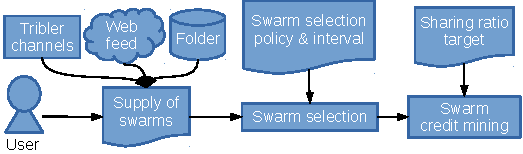
\includegraphics[width=0.8\textwidth]{pics/creditmining2015.pdf}
	\caption{The overview of credit mining process \cite{2015:creditmining:capota}}.
	\label{fig:cm15}
\end{figure}


\section{Prospecting good investment}

% emphasize on investing+prospect
Investing can not be separated by another activity called ``prospecting''. We define \textit{prospecting} as the activity to identify and measure a swarm in the hopes of getting more credit by putting a some credit as capital investment. Prospecting is the initial phase of investment, therefore, it is not needed to be comprehensive and only necessary in smaller scale. In economic perspective, not all undersupplied swarm need to be seeded, even more oversupplied swarm. Choosing a swarm to be seeded is depend on a peer available resource, intention, and investment target. In credit based community, correct investment may spark the community thus improving the performance. From user perspective, good prospecting algorithm can result a high return of the resource used from both investing and prospecting.

% crawl -> part of prospecting, knowing the swarm. 
One important part of prospecting is to identify and measure a particular swarm. Some information can be gathered by querying tracker as central coordinator. A work by \citeauthor{2011:yoshida:crawlbtnet} is the example of contacting tracker regularly to get swarm information \cite{2011:yoshida:crawlbtnet}. As the multi-tracker structure become common, they proposed to contact only one \textit{representative tracker}, which maintain the maximum number of peers in a swarm. BTWorld\footnote{\url{http://btworld.nl/}} has identified four measurement techniques in \bt~\cite{2010:btworld:wojciechowski} as shown in table \ref{tbl:btmeasuremethod}. As investment need real-time data, both \textit{swarm-level} and \textit{peer-level} measurement seems to be the most compatible with prospecting method implementation. Both \textit{internet-level} and \textit{community-level} need compiled data from ISP company and community administrators, respectively \todo{any work how to measure swarm by looking at the peers?}. 

The idea of credit mining system is to help undercapacity swarm, while at the same time to get credit for uploading data. The system try to find which swarm that might have high return by \textit{prospecting}. The investment, which relies in prospecting function, is considered with limited resources as additional requirement. Resource can be in several forms such as bandwidth, memory, or storage. Although the term ``good'' may be relative, we intend to show the efficiency of credit mining from different aspect. Therefore, we define the first research question as :

\noindent{
	\\
	\textit{How to prospect swarm and what is good investment?}\\
%	what is the properties?
	}
	
%How do we take advantage of unused bandwidth in Tribler client in non-disruptive manner?  The system address this issue by proposing activity-aware mechanism. The purpose is to get the most out of the bandwidth without disturb user of his own activity.
% What is the effect of credit mining system in live production environment?
In order to answer the question, we formulate technical challenge that need to be solved. The challenges include engineering and performance evaluation aspect. Prospecting swarm and continuously seed to gain credit may disrupt the user activity. In the other hand, it is important to take advantage of unused bandwidth. In the previous work, it is assumed that credit mining system will consume all the bandwidth. In evaluating the system, it is necessary to observe the effect of credit mining system in a whole. This can be achieved by deploying the system in live production environment. Many characteristics of swarm such as low seeder, practically dead swarm, and new published swarm will be considered. Also, the system can be improved by evaluating the properties continuously.

\section{Substituting investment cache}
In the first question, we have addressed how to gain credit as much as possible efficiently and in non-disruptive manner. However, this is not answering the limited resource available at the user disposal. In this issue, we will specifically focus on the storage limitation. The term \textit{storage} and \textit{cache} can be used interchangeably. It points to the container used to store the swarm data as the source of investment.

To start seeding, the data must be available locally in the storage. By having many data, there are higher chance to seed many swarms as well. Eventually, it is necessary to replace obsolete investment. Several reasons to do so such as gaining less profit, unstable credit, or unreliable swarm. Downloading a swarm from nothing is costly, especially if all the content need to be downloaded. Moreover, as mentioned before, it is better to avoid both underseeded and overseeded swarm because it will affect the sustainability. By replacing old swarm by the new swarm, the balance of the ecosystem must be remained stable. The method to find which swarm that has less impact to replace by the new potential swarm is needed. Although user can control the investing process, it is desirable to do this automatically. Therefore, we define the second research question as : 

\noindent{
	\\
	\textit{When to delete a downloaded swarm and replace it with a new investment?}\\
	}
	
%What is the effect of mining in background for end-user?
Technical challenge that arise by this question is covering several aspects. It related to user behavior and intention. In the prior work, a \textit{helper} system was exist. However, either it was limited to one role per peer or all the peer in the swarm have single role. While this approach is reasonable, it is unlikely that a peer will stick to one behavior. A peer may download normally from a swarm in one time, while decide to graciously help another swarm in other time. It is also currently unknown at what point the system switches from \textit{investing} to \textit{donating}, and vice versa.
\chapter{Economics in \bt}

As mentioned before, \bt~community can be viewed as social networking. Each peer represents a user. A user has \textit{needs}, which is to download a file, to be fulfilled. A file is provided by another user who has different need. This situation creates supply and demand as in traditional economics. This chapter will discuss the economics foundation formed in \bt~system.

As starters, we will discuss the concept of \textit{credit} or \textit{money} in the \bt~system, or in general, in peer-to-peer. The concept of credit is tightly related with the incentive mechanism used in P2P system to maintain the overall performance and to tackle the famous \textit{freeriding problem}. Next, supply and demand condition in \bt~system and its misalignment problem will be elaborated. Another issue which related to credit distribution that leads to system seize-up will be explained afterward. Lastly, the prospecting and investment methodology will be discussed.

The reason why user want to have a lot of credit is motivated by advantages such as higher performance. Individual and community performance must be balanced with each other. \citeauthor{2013:survivepriv:jia} mentioned that oversupply swarm will limit the possibility of giving higher bandwidth allocation for users \cite{2013:survivepriv:jia}. This phenomenon shows that although the intention from user is good, it is not the best case for the swarm perspective. Therefore, it is important for user to choose which community he want to seed to balance those interest. This chapter presents the knowledge needed to observe social-economic phenomenon and to apply suitable policy to improve the overall experience or performance.

%\todo[inline]{invest vs donate. I think we need to stick to just one of them.}

% incentive -> various, centralized, decentralized. Complicated or not. modifying bittorrent protocol? -> not standard 

\section{P2P currency and incentive}
% incentive p2p sveral forms, recipro, reputation, credit
\todo{expand:forms of incentive}

% incentive in p2p example
Incentive mechanism in peer-to-peer network is essential as it is one of the property to increase swarm performance. This statement valid in all kinds of p2p network. \citeauthor{2015:incentivep2pgame:kang} proposed an incentive mechanism for dynamic and heterogeneous peer with game theory. They take peer capabilities and selfish nature as consideration. The mechanism targeted at wireless and low computing peer which always aim to maximize its own benefit through its credit system. In their system, each peer can set a price for service it provides. The buyer (downloader), in this case, able to negotiate with the seller (uploader) regarding the content price and its bandwidth allocation. This research objective is to maximize the \textit{performance satisfaction factor} where occurred after the transaction \cite{2015:incentivep2pgame:kang}. On the other side, especially in \bt~network, \citeauthor{2010:effortincentive:rahman} proposed effort-based incentive to advocate fairness between peers. They believe that current incentive system disfavor slow peers and eventually will decrease overall performance. In this system, user awarded based on its effort, which is relative on its capacity. This mechanism need alteration in \bt~existing policy on unchoke mechanism and peer selection. However, there is an increasing performance. Download speed for slow peers increase up to 63\% at the expense of decreasing speed for fast peer at 4\%.

% what is credit -> act as a currency
When using currency as the incentive mechanism, it is necessary to define the transaction unit used between the user. In this thesis, we define it as ``credit''. ``Wealth'' is a collection of stored credit on a particular user. Several researches defined credit depend on the case they intend to solve. \citeauthor{2012:economicbt:kash} defined one in his case as \texttt{4 x upload\_bytes - download\_bytes} which is the amount of user can download respecting to DIME share ratio requirement. The credit itself is asymmetrical. From the previous case, for example, if a byte sent from A to B, A will deducted 1 credit, while B will be rewarded by 4 credit \cite{2012:economicbt:kash}. A number of owned credit usually stay linear with another metric called ``reputation'', that is, high credit lead to high reputation as well. Reputation shows how trusted and dependable a user is. 

% terms, content pricing, intro to incentive by example
In his work, \citeauthor{2012:economicbt:kash} defined many economic terms suitable in \bt~community. The \textit{price} of a file is the amount of credit deducted from downloader's wealth. This, in many cases, the same amount uploader will receive and it depend on the size of the file. Commonly, the price per bytes is the same for all the file in the community. However, \citeauthor{2012:economicbt:kash} suggest that a community should carefully declare different price for different files. One way to do it is by lowering the price for the old content, or by defining price depend on the availability and capacity \cite{2012:economicbt:kash}. Another introduced term is \textit{resale value}. Resale value is the amount of \textit{gross} credit one will get by uploading a file. In DIME case, it is 4 times uploaded bytes. In other words, resale value is the amount of return one can expect by uploading a file. We saw this mechanism as a way to incentivize user. Because by uploading one byte, a user can get 4 credit which can be used to spend/download 4 bytes.



% don't too much / lack of credit
The use of credit in \bt~environment must be implemented with utmost care. \citeauthor{2010:crashsustain:rahman} showed that credit dynamics in P2P community, especially \bt, can lead to system seize-up. There are three statuses observed: \textit{crash}, \textit{crunch}, and \textit{sustain}. Crash and crunch is the condition where there are too much credit and lack of credit, respectively \cite{2010:crashsustain:rahman, 2015:sustainabilitypt:vinko}. To preserve swarm sustainability, there are two aspects that need to be considered. The first one is the swarm condition such as file size and initial credit distribution \cite{2015:sustainabilitypt:vinko}. \citeauthor{2015:sustainabilitypt:vinko} showed that large file size could decrease the sustainability of a swarm. As for initial credit configuration, it depends on the community itself. The wrong amount can crash the system, while with the right amount overall throughput can increase. Secondly, it is the peer behavior \cite{2010:crashsustain:rahman}. \citeauthor{2010:crashsustain:rahman} concluded that selfish peer who only upload in order to continue downloading (freeriding) can badly harm the swarm. Moreover, crash and crunch situation can only be solved with external intervention.

\subsection{Tackling free rider problem}
% what is freeriding and how severe
Incentive mechanism is a straightforward method to counter freeriding and increase cooperation. Freeriding known to reduce the overall performance in peer-to-peer system. In Gnutella, 70\% of its user is not shared any files. Moreover, almost half from total communication only served by 1\% of total peer \cite{2000:freeridegnutella:adar}. If everyone can free ride, the whole system performance may degrade significantly. In other words, freeriding can lead to systematically worse problem called ``tragedy of the commons'' \cite{1968:tragedycommon:hardin}. This problem is popularized by \citet*{1968:tragedycommon:hardin} in \citeyear{1968:tragedycommon:hardin}. This social dilemma emerge because overuse and overexploitation in the shared resource without feedback from the user.

% how can egoist cooperate :  The Emergence of Cooperation among Egoists (Robert Axelrod). Solved by tit-for-tat -> good performance. managing supply and demand meulpowder p.7

% how bittorrent handle freeriding (short term)
\bt~comes with a \textit{tit-for-tat} solution to tackle this issue \cite{2003:bittorrent:cohen}. \textit{Tit-for-tat} in \bt~encourage user to only upload file to one who also has uploaded his file. Furthermore, it is also ranked by upload amount and speed. Freerider always getting low priority in this mechanism. Tit-for-tat valid only in a scope of single torrent. That means, the configuration from one community can not be carried to another community. This causes tit-for-tat works best only in short term transaction and limited parties.

% reputation system (long term)
To complement tit-for-tat mechanism, it is necessary to implement global incentive scheme in \bt. Some researchers start by leveraging the reputation system for peers. This also supported by \citeauthor{2002:reputationtotragedy:milinski} that reputation can help solving ``tragedy of the commons'' problem \cite{2002:reputationtotragedy:milinski}. The mechanism can be centralized on decentralized. Private communities that enforce SRE is an example of centralized mechanism. The reputation of user is stored in the server while it update the data in the communication via tracker. BarterCast \cite{2009:bartercast:meulpolder} and its successor MultiChain \cite{2015:multichain:norberhuis} are the example of decentralized incentive mechanism that works on top of reputation system. 

% freerider behaviour, tit-for-tat result
\citeauthor{2015:freeriderinbtcommunity:das} studied the freerider behavior in \bt~communities. They conclude that freerider in \bt~may not degrade performance as long as the swarm has at least one dedicated and available seeders. The potential availability of seeder also become a factor that keeping the swarm alive. One thing that need to take into consideration is that in their research, they only take four communities as dataset \cite{2015:freeriderinbtcommunity:das}. In \bt, it is unlikely a user will be extremely freeriding, that is not upload anything while keep download data. More common case is the \textit{hit and run} behavior \cite{2011:managesupplydemand:meulpolder}. Hit and run (HnR) is a situation where a user has finished downloading then immediately stop his contribution. Hit and run also often referred as one of the freeriding behavior that peer-to-peer community wanted to prevent.

% cite : The Bittorrent P2P File-Sharing System: Measurements and Analysis

% may include limitation on the effectiveness meulpolder
%Require the change of the system :  \cite{2008:givetogetvod:Mol}. \cite{2010:effortincentive:rahman} \cite{2015:incentivep2pgame:kang}.
% user impossible to be altursitic, not necessary be paranoid. Fairness and system design. While may be reduce performance in spsecific case.

\section{Supply and Demand}
% supply < demand
Supply and demand for both public and private \bt~communities have been studied by \citeauthor{2009:demandsupplyres:andrade} in \citeyear{2009:demandsupplyres:andrade}. \citeauthor{2009:demandsupplyres:andrade} shows that user who contribute more to the community, actually consume a lot from it. This explains that \bt~users are not altruistic enough to seed continuously. Although a significant amount of demand is successfully served by the community, there is only a few swarm that does not suffer from contention. Two hypothetical reasons \citeauthor{2009:demandsupplyres:andrade} suggested are: (i) an asymmetric number of seeder and leecher, which seeder cannot compensate; and (ii) lack of incentive mechanism in the higher level aside from \bt~\textit{tit-for-tat} \cite{2009:demandsupplyres:andrade}. 

% supply in private > in public; flashcrowd increase demand
In public community, there is less supply compared to private community which enforce SRE \cite{2009:demandsupplyres:andrade}. This affects a file longevity because user seed longer in private community. If this behavior happened in long period, it might produce significant imbalance on supply and demand as seeder kept seeding a particular torrent without switching to another swarm. This phenomenon is accumulated by existing of \textit{flashcrowd} effect. Flashcrowd effect is the sudden increase in resource demand due to various reason. Newly published torrent is one of the reasons where flashcrowd effect take place \cite{2013:swarmevolution:su}. These misalignments between supply and demand can worsen the downloading experience in \bt.

% undersupply vs oversupply
In classical file-sharing peer-to-peer system, it is common to see that a swarm is \textit{undersupplied}. Undersupply means that there are not enough resource shared within the swarm to be distributed over the peers who wanted it. The reason why a user join a swarm is to download a file, so that is why undersupplied is commonly occurred. However, with the introduction of private community which enforce upload policy such as SRE or reputation mechanism, the problem shifted to a phenomenon called \textit{oversupply}. Both undersupply and oversupply is the sub-case of supply and demand misalignment. Undersupply condition can be solved by adding more high performance peer to boost download experience. In the other hand, oversupply problem is not trivial to solve.

% oversupply -> fierce upload competition -> unbalance situation
In oversupplied swarm, user may find it difficult to earn the credit by uploading the file. This is because the problem described by \citeauthor{2011:managesupplydemand:meulpolder} called ``upload competition'' \cite{2011:managesupplydemand:meulpolder}. Two conditions from peers perspective must be fulfilled to make P2P system sustain, which is peers must be cooperative, and cooperative peer must stay as long as possible in the swarm \cite{2011:managesupplydemand:meulpolder}. In upload competition problem, cooperative peer can not control his upload rate. The one who will download the seeder chunks is out of the seeder knowledge and control. This may result an expulsion from the community with a SRE because the cooperative peer looks like it do not contribute. \citeauthor{2010:crashsustain:rahman} also stated that oversupply may result to system seize up by \textit{crashing}  \cite{2010:crashsustain:rahman}. Sustainability of a swarm is in a risk in this situation.

% balance -> not sustain
\citeauthor{2011:managesupplydemand:meulpolder} in his work illustrated the relation between various P2P system properties and its relation to system balance. The illustration shown in figure \ref{fig:sysbalance}. Request and seeding behavior is another term of user downloading and uploading behavior, respectively. Seed selection is one part that responsible for choosing which peer to seed. In \cite{2011:managesupplydemand:meulpolder}, \citeauthor{2011:managesupplydemand:meulpolder} showed that using naive random seeding behavior is not sufficient to make P2P system balance. Unbalance system can lead to unsustainable community. Therefore, it is important to work study seeding behavior for each peer by the implementation of credit mining.

\begin{figure}[ht]
	\centering
	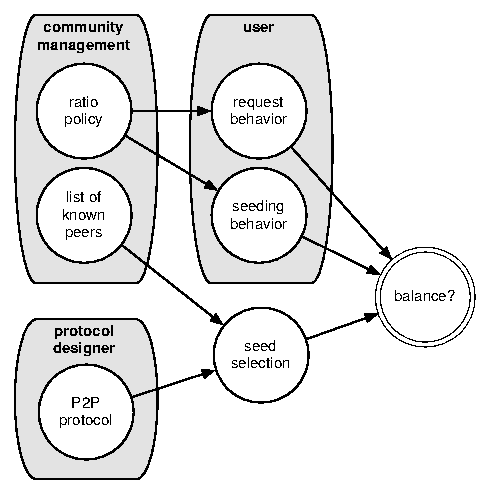
\includegraphics[width=0.7\textwidth]{pics/p2psys_balance.pdf}
	\caption{System properties and its relation to P2P balance \cite{2011:managesupplydemand:meulpolder}.}.
	\label{fig:sysbalance}
\end{figure}


\section{Prospecting and Investment}
% the importance of healthy swarm -> public good, prevent tragedy of the common

% helping others in p2p, improve performance
Recent work on helping other user or increasing downloading performance using \bt~ has been done. \citeauthor{2014:cloudseed:leon} uses \bt~ protocol to increase user download speed and at the same time reduce datacenters load. They analyze which swarm or file to help using user bandwidth information and number of connected user\cite{2014:cloudseed:leon}. From another perspective, \citeauthor{2015:coalitionbt:zhang} introduced the \textit{coalition} between \bt~ peers. Coalition is a set of peers that cooperate each other in regards to \bt~policy to minimize download completion time. They also propose coalition-compatible choking strategy to replace the current \bt~one. This research lead to significant performance improvement within the coalition \cite{2015:coalitionbt:zhang}. Although not using \bt~protocol, in \citeyear{2009:p2phelp:he}, \citeauthor{2009:p2phelp:he} proved that helper peer also can improve the streaming capacity in P2P system\cite{2009:p2phelp:he}. \citeauthor{2016:gameauctionp2pstream:mostafavi} extend this work by introducing auction aspect for uploader to choose which user will receive the bandwidth he donate \cite{2016:gameauctionp2pstream:mostafavi}. \citeauthor{2016:gameauctionp2pstream:mostafavi} used game-theory to propose new framework in uncooperative peers with maximizing the credit gain for helpers.

% user is selfish, it is good to donate. Reality : they want something in return -> credit. Move the problem into investment problem. Distinction invest vs donate.
%We define the activity of seeding with the expectation of obtaining credit to use later on as \textit{investment}. The act of seeding to help to increase the community performance graciously is called \textit{donating}. A user can \textit{prospect} which community he will invest or donate regardless of his own resource. Not all the swarm need to be seeded as we shown the drawbacks of oversupply. The prospecting and identifying swarm that needs to be seeded based on the seeder's intention (whether to invest or donate) is important. By providing proper prospecting function, users could help each other to improve the swarm quality. In good investing algorithm, users can make better use of its resource to gain credits when prospecting a swarm. 


Crawl bittorrent network \cite{2011:yoshida:crawlbtnet}. More can be seen in \cite{2010:btworld:wojciechowski}.

Resale value \cite{2012:economicbt:kash} related to torrent age. 


\chapter{Credit Mining System Design}
\label{chp:design}

% section overview, main components. Libtorrent as dependency. 
The goal in this thesis is to implement and evaluate a system where it can be used to both invest credit and improve swarm performance. In this thesis, we introduce ``Credit mining system'', an automatic investment framework on swarm with multidimensional gain. With credit mining system, locally, a user can gain credit with internally limited bandwidth allocation without any intervention needed. The credit can be in many forms such as share ratio (upload-to-download ratio), uploaded amount, effort based credit, and many other. From higher perspective, credit mining system will help a swarm to keep alive by providing integral pieces to the peer who need it. Although credit mining system will be implemented in Tribler system, it is possible to apply this feature to any file-sharing system.

Firstly, the dependencies of credit mining system which is \textit{libtorrent}'s s\textit{hare mode} will be elaborated. \texttt{Share mode} is a module which can be activated as an intent to helping a swarm instead of normal content downloading. This module will be explained in detail in section \ref{section:sharemode}. The rest of the section \ref{section:libtorrent} explain other relevant, yet important module that credit mining system can exploit. Afterwards, the design of credit mining system is presented. This system consists of several subroutines which will be explained afterwards in section \ref{section:cmcomponents}. 

\section{Libtorrent}
\label{section:libtorrent}
With \bt~is just a collection of specification, it free to be implemented with any languages. One of most popular implementation is \textit{libtorrent}. \textit{Libtorrent} is written in \texttt{C++} and adopt open-source policy. \textit{Libtorrent} also has \texttt{python} binding which the same language as Tribler implementation. \textit{Libtorrent} started in 2003 by Arvid Norberg and it implemented most of the \bt~specification. Most of the crucial specification such as DHT, IPv6 tracker, PEX, magnet link, multi-tracker, webseed, and many others has been implemented. That is why \textit{libtorrent} is widely used by many torrent client such as Deluge, qBittorrent, Free download managers, and many others.

In this section, we will elaborate some of the \textit{libtorrent} feature that used in credit mining system and within our scope. How priority is managed within \textit{libtorrent} will be explained. After that, \textit{share mode} as the core function we needed is described in detail. The relation to credit mining system with it will be explained to both of them. In the last part, we will focus on the several peer discovery techniques. With the trackless \bt~evolved in early 2008 by DHT protocol \cite{2008:dht:loewenstern}, monitoring trackers may result in inaccurate result. Moreover, the credit mining mechanism heavily rely on real-time data which can not be obtained from querying the community pages. The data can be acquired both directly and indirectly by crawling peers in the swarm.

\subsection{Priority Management}
Determining which part of the file that needed to be downloaded is central component in \bt~implementation. By default, \textit{libtorrent} will look for rarest piece available in the swarm. However, it is possible to change this behavior. \textit{Libtorrent} provides an API with high granularity. Within a \textit{libtorrent} session, a swarm may have different priority compared with other swarm. Higher priority means higher chance to get unchoked. It is done by enlarging peer's bandwidth who has that swarm. In this way, \textit{libtorrent} can always prioritize those peers, therefore, the particular swarm. 

Going deeper into \textit{libtorrent} API, it is also possible to prioritize a particular files or pieces in a swarm as well. It is common to have multiple files assigned in a swarm. A file consists of many pieces. However, one piece may represent one or more file. In a swarm perspective, length of the piece is always same, except the last one. By prioritizing files, \textit{libtorrent} assigned all pieces correlated with that file. Assigning priority to a piece will affect how that piece will be chosen for downloading. By default, \textit{libtorrent} sort the piece by its availability. Therefore, it downloads the rarest piece first before anything else. The piece and file priority can be overridden by calling the API. There are 8 level of priority, with level 0 means never be downloaded. The levels are : 

\begin{enumerate}[topsep=1pt,itemsep=0ex,partopsep=0pt,parsep=2pt]
	\itemsep0em 
	\item[0.] piece is not downloaded at all.
	\item normal priority. How \textit{libtorrent} download it is depending on the piece availability.
	\item higher than normal priority. \textit{Libtorrent} prefer this piece instead of other piece which has same availability
	\item in partial piece mode, picker will prefer to pick this priority on top of other priority
	\item in partial piece mode with the same availability, picker will pick this piece instead of \textit{3)}
	\item this priority is the same as \textit{4)}
	\item this piece is likely to be picked as long as the availability is more than 1
	\item maximum priority. Picker will not consider availability and always prioritize this piece.
\end{enumerate}

Using the mentioned API, credit mining system independently prioritize part of the swarm with various conditions. As will be shown in Section \ref{section:optimization}, the system always prioritize the user downloading activity rather than its mining activity. In other condition, credit mining will trigger the idle mining activity and do an initial download part to measure the swarm. This feature shown later in Chapter \ref{chapter:prospection}. 
%Unchoke round. Bandwidth control.

\subsection{Share Mode}
\label{section:sharemode}
One of the crucial feature used in this work is \textit{share mode} \footnote{Core code of share mode can be found in \url{https://github.com/arvidn/libtorrent/blob/master/src/torrent.cpp\#L9586-L9727}}. Initial work performed by \citeauthor{2015:creditmining:capota} also used this feature\cite{2015:creditmining:capota}. By enabling share mode, it means that one is not interested in downloading the file, but gaining higher share ratio. It is done by download as little as possible and upload as much as possible. Share mode only download a torrent where it has sufficient capacity. A torrent downloaded in share mode may never finish as \textit{libtorrent} only download piece of a torrent which satisfied the share mode requirements. Share mode can be enabled per torrent basis.

Share mode algorithm works heuristically as it estimates the rarest piece available in the swarm based on participated peers. First, it tries to find whether there is a piece which nobody has (line \ref{alg:l_lts:missingp}). Note that in line \ref{alg:l_lts:disconnectpeers}, libtorrent disconnect some of the seeder because we need to connect to the leecher later. This case is considered if there are too many seeder in our connection pool. Next, the number of missing pieces is decreased linearly with the number of seeder. This is based on assumption that both of us and other seeder can upload at least one piece each (line \ref{alg:l_lts:reducemissing}). To keep the performance, downloading piece activity is stacked until more than 5\% of the number to be downloaded (line \ref{alg:l_lts:retdling}). To determine rarest piece, libtorrent count the number of peer that has that piece. The number of peer on the rarest piece is termed \textit{rarity}. Share mode ensure that we only download the rarest piece available in the network (line \ref{alg:l_lts:rarepc}). We end the prematurely routine if there are more number of piece to download compared to uploaded (line \ref{alg:l_lts:retdlenough}) or there are not enough peer to upload the rarest piece (line \ref{alg:l_lts:rareunable}). Both condition will prevent us to get positive share ratio. Finally, it will download randomly the rarest pieces if there are more than one option (line \ref{alg:l_lts:dlrare}). The algorithm presented in algorithm \ref{alg:ltsharemode}. 

\begin{algorithm}[h!]
	\caption{Libtorrent share mode algorithm}
	\label{alg:ltsharemode}
	\begin{algorithmic}[1]
		\Require{$T$ as share mode target}
		\Statex
		\State{$missing\_piece = 0$}
		\ForAll{$p \in connected\_peers$}
		\If{$p$ is a $leecher$ $and$ $p$ is not in share\_mode}	
		\State{$missing\_pieces$} += {$total\_pieces - pieces(p)$} \label{alg:l_lts:missingp}
		\EndIf	
		\EndFor
		\If{$|connected\_seeders|$ in $connected\_peer$ $>$ $90\%$}	
		\State disconnect excess seeder \label{alg:l_lts:disconnectpeers}
		\EndIf
		\State{$missing\_pieces$} -= {$2 \times |connected\_seeders|$}	\label{alg:l_lts:reducemissing}	
		\If{$missing\_pieces \leq 0$}
		\State \Return
		\EndIf
		\If{$num\_downloaded \times T > uploaded$} \label{alg:l_lts:retdlenough}
		\State \Return
		\EndIf
		\If{$downloading > 5\% \times num\_downloaded$} \label{alg:l_lts:retdling}
		\State \Return
		\EndIf
		\ForAll{$pc \in pieces()$}
		\If{$pc$ not in $collected\_piece$ $and$ $peer\_count(pc) \leq rarest\_rarity$ }	\label{alg:l_lts:rarepc}
		\State{$rarest\_rarity$} = {$peer\_count(pc)$} 
		\State{$rare\_piece$.push($pc$)}
		\EndIf	
		\EndFor
		\If{$|connected\_peers| - rarest\_rarity < T$} \label{alg:l_lts:rareunable}
		\State \Return
		\EndIf
		\State download {$random(rare\_piece)$} \label{alg:l_lts:dlrare}
	\end{algorithmic}
\end{algorithm}

There are several limitations on this feature as we observed. First, it only has single parameter which determine the desired target of share ratio. This limits the exploration and full use of share mode feature. Another issues are storage and network inefficiency. If enabled, share mode works by downloading popular piece of a particular torrent. This means few downloaded pieces could take a large storage. Share mode also did not check whether a swarm is efficient enough to perform this operation. It only tries to find popular pieces regardless of the swarm condition. It is highly possible that if a swarm is in poor capacity, the uploading rate is very low. The bandwidth used to check torrent pieces regularly is wasted and the ``investment'' will not go well. The biggest limitation of share mode is the probability of getting bottleneck because of its strict policy. In early stage of joining a swarm, share mode downloaded 1 piece at a time. This can result slower decision making and the rarity of pieces changed. 

Bottleneck can happen in the early time of share mode. The combination of line \ref{alg:l_lts:retdlenough} and \ref{alg:l_lts:retdling} will hold downloading any piece if the uploaded amount is not enough based on the piece we have. Let say we already which piece to download from line \ref{alg:l_lts:dlrare}. In the next round, this piece is not rare anymore. Therefore, we cannot upload this piece.  \todo{expand}
% peer discovery DHT, PEX, LSD
\subsection{Peer Discovery}
One of the integral part in \bt~protocol is peer discovery. With numerous known peers, the algorithm will have more option on which peer to unchoke. State of the swarm itself often represented by the peer belong to that swarm. It is relatively costly just to discover new peers if there are a lot of swarms monitored. \citeauthor{2012:milliontorrent:arvid} shows an example how costly the \textit{announce} request accompanied by \textit{response} payload can be in seeding a lot of torrents. Seeding 1 million torrents with announce once per every hour, which is half of the default interval, need 130 kB/s upload and 75 kB/s download bandwidth constantly \cite{2012:milliontorrent:arvid}. This value is significant for most of common Internet connection.

In \bt, there are four methods to discover new or update peer. Those are using centralized trackers, distributed hash table (DHT), peer exchange (PEX), and local service discovery (LSD). The methods will be described below. To be able fully trackerless, \textit{magnet link} extension is needed in every peer \cite{2008:magnet:hazel}. By magnet link, user can join a swarm and complete the download without using \texttt{.torrent} as its initial data. 

\subsubsection{Tracker Peer Announce}
In original design of \bt, it uses tracker to allow peer discover each other \cite{2003:bittorrent:cohen}. Tracker tends to use random and limited list of peers. Peer contact tracker periodically to expand their peer dictionary. This act of requesting peer to tracker is called \textit{announce}.	Usually, most tracker has a policy about recommended interval when to recontact for getting new peers. Violate this policy can result a particular peer blocked.	

\subsubsection{Distributed Hash Table (DHT)}
Originally, peer needs to contact tracker to fetch new peer address and file information. This makes \bt~very dependent on centralized system which vulnerable to single point of failure. In 2008, Distributed Hash Table (DHT) was proposed \cite{2008:dht:loewenstern}. Towards a ``trackerless'' \bt~system, DHT allows each peer to become a tracker. DHT stores peer contact information with defined key-space as ``node ID''. Each peer stored other peer's node ID and its address in their own routing table. A ``distance'' is measured on two node ID to define how close those two. ``Distance'' also can be measured between infohash of a torrent and node ID.

To enrich its peer dictionary, a node can compare a torrent's infohash and node ID in its routing table. If the distance under the threshold, it contacts that node to ask the information of the swarm, which includes the peer list. If contacted node do not know this torrent, it will respond with another node in its table which closest to the provided infohash. 
%\todo{expand_:DHT performance?}

\subsubsection{Peer Exchange (PEX)}
To increase the chance of getting higher downloading speed, having up to date peer is desired. This can be achieved by contacting tracker or using DHT. Reducing the interval of contacting tracker can result in getting a number of updated peer sooner, however, it will put a burden on the tracker itself. Peer Exchange (PEX )\cite{2015:PEX:the8472} is proposed to tackle this problem. PEX used list of peers that bootstrapped from another mechanism. This mechanism allows contacting known peer directly to get and give up-to-date information on swarm. Theoretically, it can keep this swarm together if trackers are down. Specification mentioned in \cite{2015:PEX:the8472} stated a restriction such as number of request per minute and number of peer added or removed in a PEX message.

\subsubsection{Local Service Directory (LSD)}
To increase the performance when downloading from a swarm, it is preferable to get the file from local network if available. Local service directory (LSD) permit this by discover peers that are in the same local network. The transfer rate is much higher compared to other type of peers. In short, LSD uses multicast-like mechanism which broadcast infohash of a torrent.


\section{Credit Mining Architecture}
\label{section:cmcomponents}

Credit mining system is intended to do its task automatically with minimal user intervention. The way this system designed is to align supply and demand of chosen swarm. Short term advantage of this approach is to gain credit by minimal download and maximize upload. In the long term, this potentially increase overall performance of other user as well.

The system can be implemented beside any torrent client. In Figure \ref{fig:cmcomponents}, it shown the compulsory elements and the relation between \textit{credit mining system} and \textit{torrent client}. Currently, we assume that every torrent client also track how much data a user has been downloaded and uploaded. We called this tracking history as \textit{credit storage} or \textit{bank}. Naturally, any torrent client must have \textit{downloading module} as well. Other dependency are te \textit{libtorrent} library. Credit mining system will use some of the \textit{libtorrent}-specific function. This function is not part of the \bt~Enhancement Protocol (BEP) which define the standard of \bt~protocol that need to be implemented. Other required feature is the ability of discovering peer by all method (DHT, PEX, LSD, etc). In some cases, peer discovery function is disabled for security reasons. While disabling one should not affect credit mining system, it will reduce the prediction and overall performance.

Credit mining system consists of several elements. First is the \textit{credit mining manager}. The \textit{manager} receives the \textit{settings} from user in the initial phase. To control mining process, user can only interact with value at \textit{settings} elements. User also limited to only add and remove \textit{mining source}. Each of the source will be assigned with a \textit{miner} depend on the type of the source. Miner also has sub-elements as part of the system. In-depth explanation of mining source and miners will be discussed in Section \ref{section:msource}. We introduce the \textit{predownload} mechanism as a way to evaluate a source early. This mechanism is launched by the manager instead of miner as it only happen during \textit{early propecting stage}. Predownload mechanism and prospecting methodology in general will be discussed in Chapter \ref{chapter:prospection}.

\begin{figure}[ht]
	\centering
	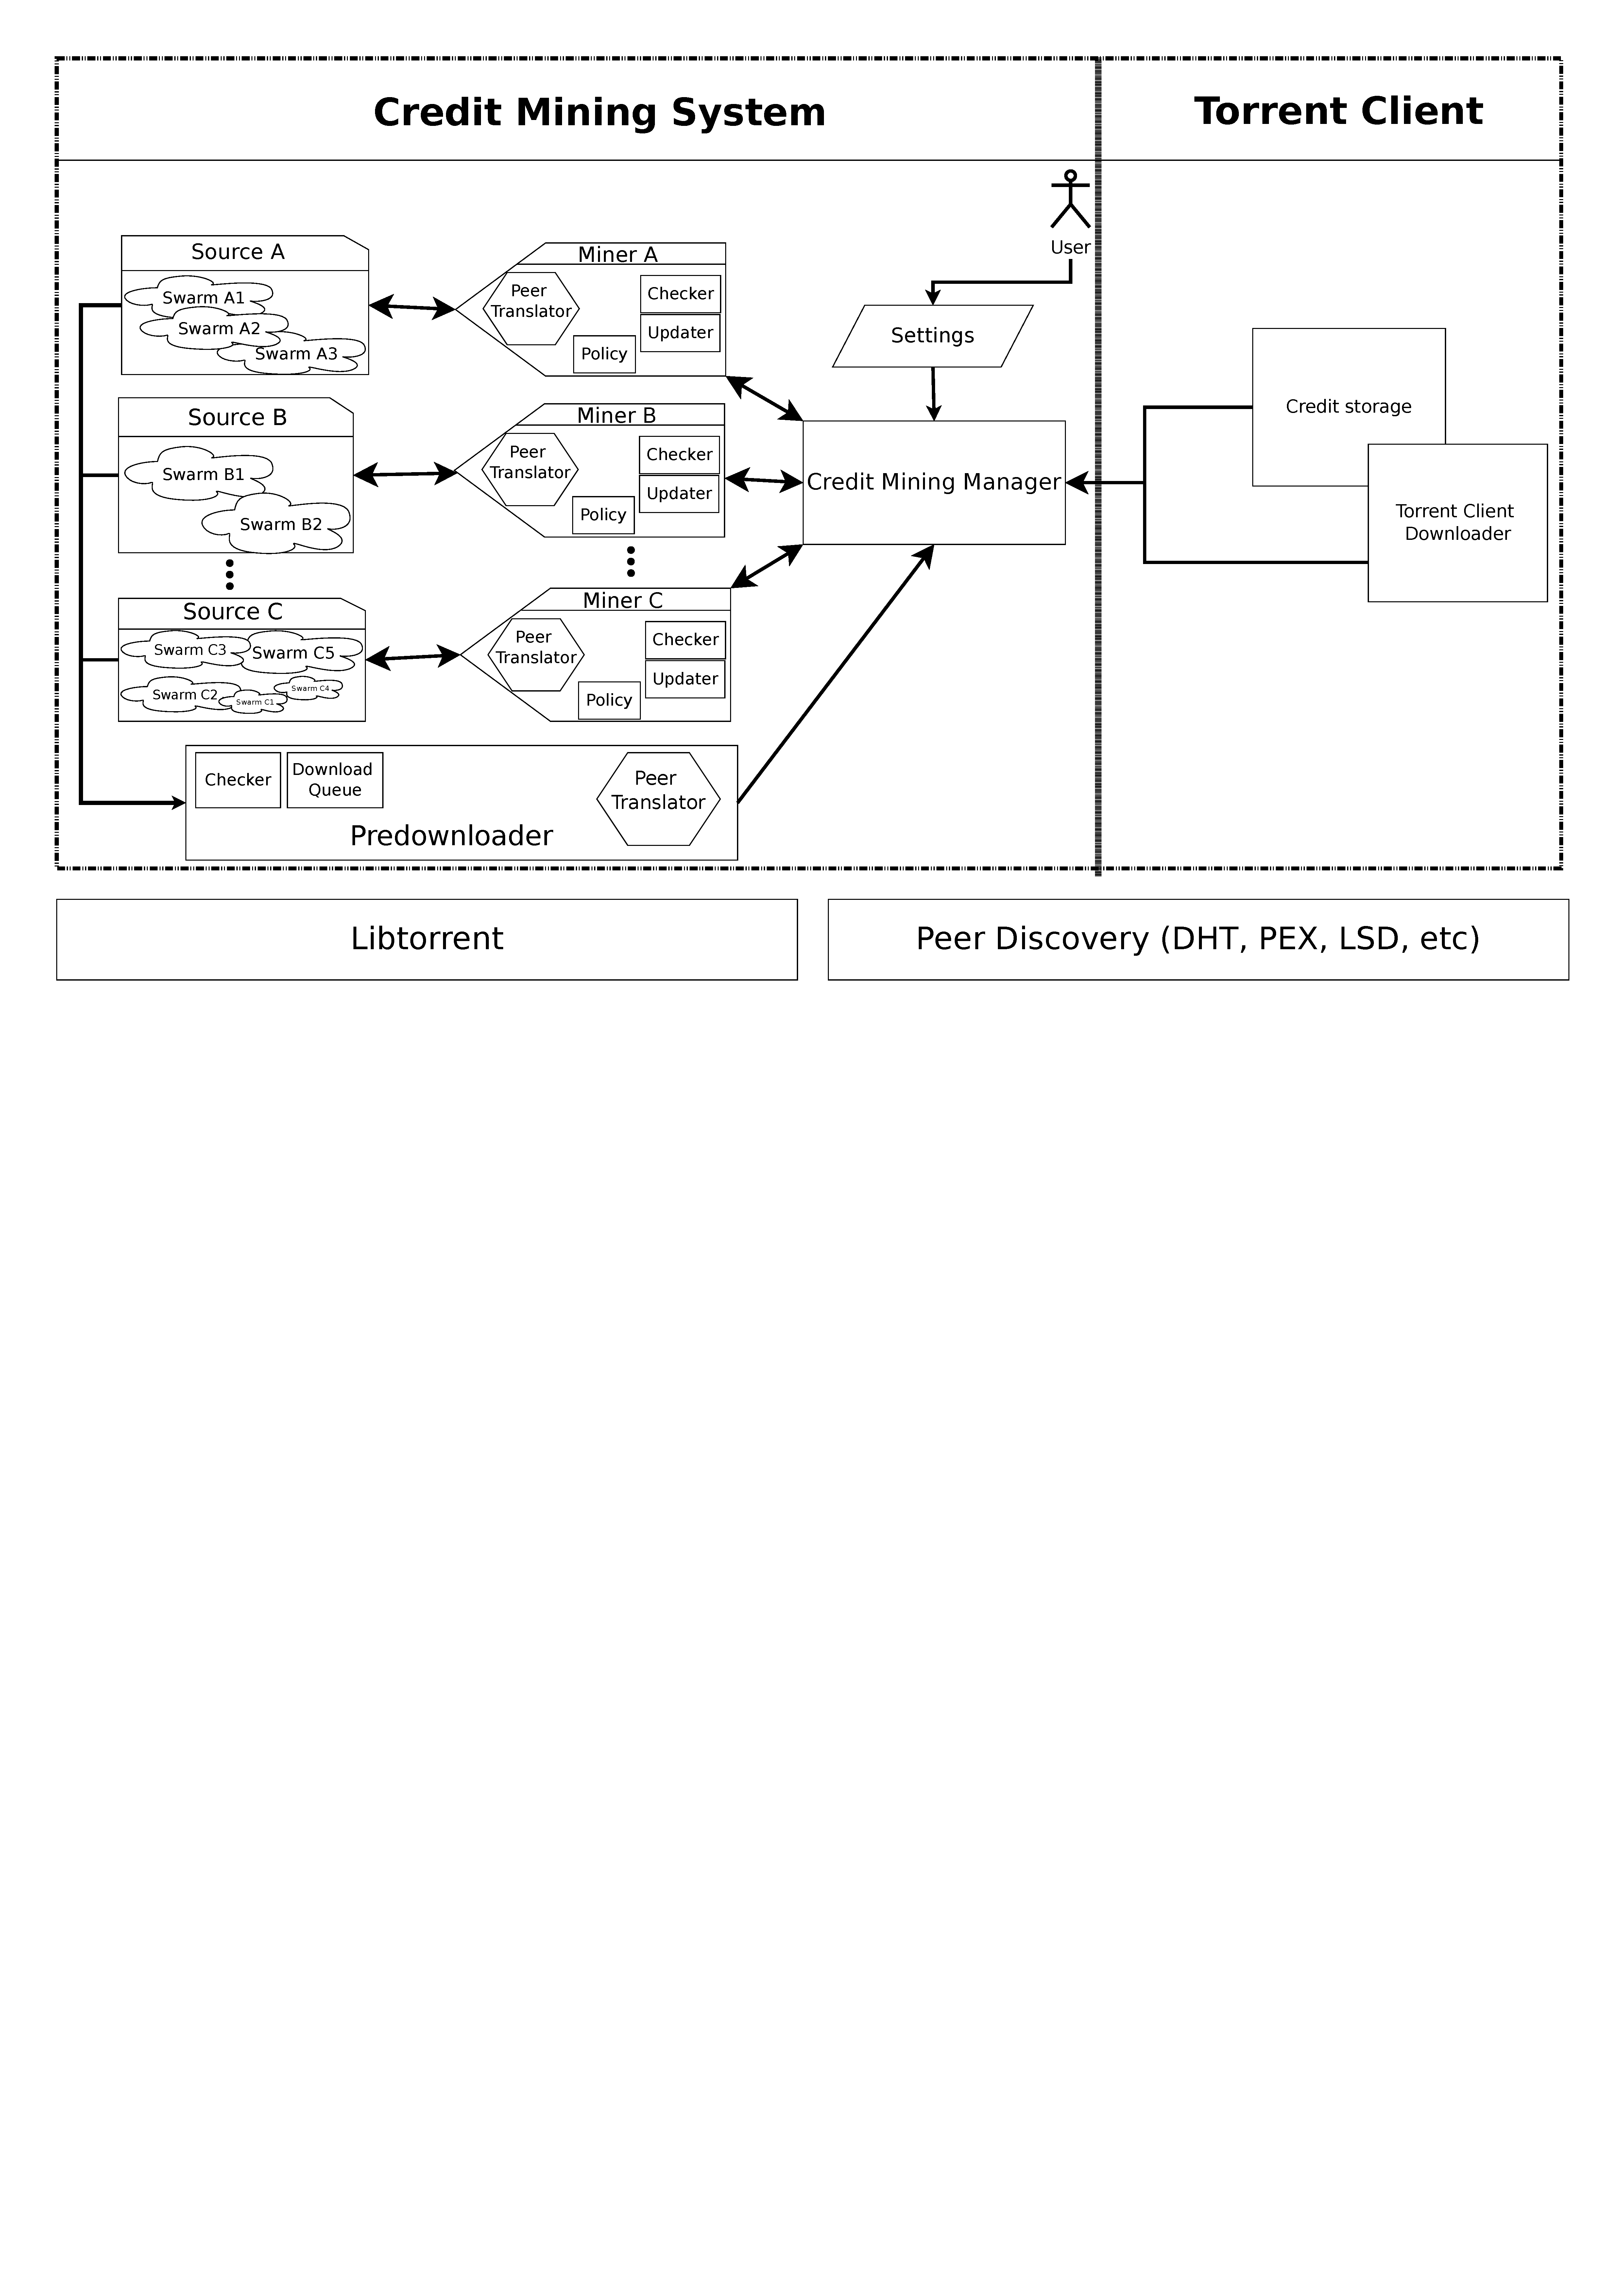
\includegraphics[width=\textwidth]{pics/cm_components.pdf}
	\caption{Credit mining components.}
	\label{fig:cmcomponents}
\end{figure}

% general flow
First, user can change the default settings used in the credit mining system. Some can not be changed when mining process run already. Table \ref{tbl:cmsettings} shows the settings used in this system. After user provide the setting and run the \textit{credit manager}, user can start mining by adding sources. A source usually consists of several swarms with different size, availability, and capacity. Each of the swarm will be assigned with one \textit{miner} that may have different type depends on the swarm itself. Before the miners start mining, \textit{predownloader} try to fetch swarm information as much as possible then give the results to the manager. Manager will propagate the swarm information to miners and let the miners decide which swarm to mine based on that information. Manager also monitor the main torrent downloader to adjust swarm's priority in miners. The credit gained from each of the miner will be reported to manager, then it forwards the results to credit storage in torrent client if necessary.

\begin{table}[h]
	\centering
	\caption{Credit mining settings}
	\label{tbl:cmsettings}
	\begin{adjustwidth}{-1.5cm}{}
	\begin{tabular}{|p{1cm}|p{4cm}|p{7cm}|p{2cm}|}
		\hline
		\rowcolor[HTML]{EFEFEF} 
		No. & Name & Description & Changeable at runtime \\ \hline
	1 & \textit{max\_torrents\_active} & The maximum number of simultaneous swarm that will be downloaded & Yes \\ \hline
	2 & \textit{max\_torrents\_per\_source} & The maximum number of stored torrent in a miner that will be considered for mining & Yes \\ \hline
	3 & \textit{source\_interval} & The interval needed to check for updates in the swarm & Yes \\ \hline
	4 & \textit{swarm\_interval} & The interval to re-evaluate swarm and start/stop swarm & Yes \\ \hline
	5 & \textit{share\_mode\_target} & Libtorrent share mode target (See Section \ref{section:sharemode}) & No \\ \hline
	6 & \textit{policy} & The policy used in mining (See Chapter \ref{chapter:prospection}) & No \\ \hline
	7 & \textit{logging\_interval} & The interval for logging, for debugging purpose & No \\ \hline
	8 & \textit{tracker\_interval} & The interval to check for a new peer by peer discovery methods & No \\ \hline
	9 & \textit{timeout\_torrent\_activity} & The maximum time threshold to mark a swarm as 'inactive' & Yes \\ \hline
	10 & \textit{piece\_download} & The number of piece what will be downloaded in \textit{predownload} phase & No \\ \hline
	\end{tabular}
	\end{adjustwidth}
\end{table}

Credit mining system is designed to be highly customizable. Some of the components can be extended or replaced. For example, the policy used to select the swarm. Beside what we proposed, user can define the policy as long as it overrides a function that return which swarm to start and stop. For peer translating, it is possible to override the function considering peer list and its information as an input, while returning number of seeder and leecher. Some value in the settings can be adjusted to match user's need and resource. With higher memory available, it is desirable to mine many swarms in one time by changing \textit{max\_torrents\_active} parameter. By having large storage, increasing \textit{piece\_download} may result a better return.

%The rest of this section will discuss key points of credit mining system. Several mining source types are supported with different treatment from miners. Prospecting methodology on top of libtorrent share mode will be elaborated afterwards. The methodology consists of two integral stages. Each of the stage has their own mechanism and requirements. Lastly, we will discuss other components that can support credit mining system of its prospecting, performance, and credit gain. 

\subsection{Mining Sources}
\label{section:msource} 
Currently, credit mining can accommodate three types of sources. There are directory source, RSS source, and channel source. In credit mining system, one source is assigned to one miner. The miner will start working the moment the source is defined and added to the manager. A miner periodically perform checking and other operations on all the torrents in the source. The operation that run in specified interval implemented differently for each of the source type. 

First type of source which called \textit{directory source}, is very straightforward. It takes a path as an argument and verify it before run the miner. The miner starts by looking at all the file in specified directory that have \texttt{.torrent} file type. Each of the file is examined and validated. Corrupt or invalid file will be discarded and deleted automatically from the disk. To keep the performance and prevent disk bottleneck, the miner sort the files alphabetically and put it into queue one by one. Miner periodically monitor both the directory if there is a new file and the queue to assign it to the manager. Miner eventually will pop an item from the queue, build a suitable format for mining, and notify manager to include this swarm.

Next possible mining source is from RSS (Rich Site Summary). RSS is a well known method to fetch new published data from a web. An RSS document contains the list of affected content which usually has summarized text and metadata. XML (Extensible Markup Language) format is widely used in RSS because of its compatibility and efficient size. An RSS from torrent portal such as etree\footnote{\url{http://bt.etree.org/rss/bt_etree_org.rdf}} and mininova\footnote{\url{http://www.mininova.org/rss.xml}} usually have title, publication date and a link to the swarm. Some mention number of seeder and leecher in the document. We called a source of RSS document as \textit{RSS feed}. 

In \textit{RSS source}, we assume that the RSS link user provided is available. If by any case the retrieval of the content is failed, the miner will stop immediately, notify the manager to disable this source, and shutting down itself. If the initial content retrieval is success, update mechanism will be launched periodically. In this mechanism, miner will fetch newest content from RSS feed. This content then parsed, resulting a list of swarm link and its metadata. Miner then asynchronously download the complete swarm data either via \texttt{.torrent} or magnet link. The same link will not be downloaded twice. After fetching the data, miner will build a defined format for mining, and notify manager to include this swarm. This data held across session. That means, another miner also will not download this swarm data in case it is indexed by other RSS feed.

\textit{Channel source} is the last type of source which tightly related to Tribler environment. As mentioned in section \ref{section:tribler} (Table \ref{tbl:community}), channel is responsible for managing torrents and playlists in Tribler community. A single channel can be discovered in \textit{AllChannel} community. Channel is identified by unique 40-length hexadecimal string. Naturally, Tribler user can create their own channel, put torrents into the channel, and share to other user. It is also possible for user to add a torrent to another user's channel. When a user subscribe to a channel, they will be notified if new torrent is added into that channel. Moreover, the torrents will be automatically downloaded into Tribler's database.

The flow of channel source is quite different with other type of source. It is tailored to follow Tribler specification which can change in the near future. Provided the identifier of a channel, miner will continuously try to find and join the channel in \textit{AllChannel}. By joined the channel, miner can get the list of torrents and other of its properties. After miner joined the channel, the swarm information will be handled and downloaded by Tribler. What miner do is to monitor the local database whether a new data has been fetched and there is a space for adding possible new torrent to the manager. Providing the swarm information, miner will download the \texttt{.torrent} file. It can be downloaded by using several options such as DHT, magnet link, or download from Tribler peers using TFTP (Trivial File Transfer Protocol). Downloaded \texttt{.torrent} will be stored in Tribler database. Afterwards, the mining format will be built and manager will be notified of a ready swarm.  

\subsection{Resource Optimization}
\label{section:optimization}
In this section, we focus on several optimizations that can be implemented in credit mining system. These optimizations are optional and can be left out. However, as the system itself is not without flaws, an improvement to support this system is advantageous. In general, there are two categories of support : helping get more credit in swarm and improving system resource utilization. The summary of designed optimizations are shown in Table \ref{tbl:optimizations}.

\begin{table}[t]
	\centering
	\caption{Credit mining optimizations}
	\label{tbl:optimizations}
	\begin{adjustwidth}{-1.5cm}{}
		\begin{tabular}{|p{0.7cm}|p{4cm}|p{10cm}|}
		\hline
		\rowcolor[HTML]{EFEFEF} 
		\hline
		\textbf{No} & \textbf{Optimization}& \textbf{Short Description} \\ \hline
		1  & Eliminate duplicates  & Removing identical files in swarm to mine \\ \hline
		2  & Swarm blacklisting    & Avoid picking slow swarm that has been previously invested\\ \hline
		3  & Inciting Swarm & Optimistically download new rarest piece if it idle too long\\ \hline
		4  & Starvation prevention & Immediately stop a swarm that idle for a long time and replace it with another one\\ \hline
		5  & Fallback mechanism    & Always pick \textit{default policy} whenever no swarm started although there are slots available \\ \hline
		6  & Reusing cache         & Reusing downloaded content when restarting the swarm instead start from nothing \\ \hline
		\end{tabular}
	\end{adjustwidth}
\end{table}

\subsubsection{Economic gain support}
In preliminary work by \citeauthor{2015:creditmining:capota}, credit mining system able to distinguish duplicate content in the P2P communities. It is highly possible that an exact same file have different infohash. An infohash of a torrent can come from many aspects such as different piece size, categorized as private or public swarm, or even directory name of the files \cite{2015:creditmining:capota}. We used \textit{Levenshtein distance} to measure the different between one swarm and another by considering the files and its length. In the end, we only mine the one who has higher number of seeder. The swarm comparison executed whenever there are new swarm reported by the miners. By eliminating duplicates in P2P communities, the supply and demand of a particular file can be focused. By focusing supply and demand into few swarms, the performance of participating peer might be improved \todo{Exclude archive mode in mihai's work because the implementation is not clear}.

In prospecting, it is possible that not all the swarm prospected can have good results. Regardless of the policy used, every miners will try to find best swarm in their library. In \textit{scoring policy} for example, miner will always try to mine best swarm found although it has very low score. In \textit{seeder ratio policy}, as long as there are peers in the swarm, a swarm will have a chance to be mined. On one hand, it is difficult to measure a swarm without joining it first, that is by downloading and seeding in that swarm. On the contrary, optimistically mine swarm may lead to sub-optimal performance. We argue that this is not necessarily a bad thing. By \textit{swarm blacklisting}, low performance swarm can be flagged and avoided in a longer term. Miner periodically check the performance of its swarm. \textit{Swarm blacklisting} also run in that period. Miner watch the when a particular active downloading or uploading data. If no activity detected in a swarm in a long period of time, the miner will remove this swarm from its library, Note that the swarm has a chance to be added to library again after several rounds. Moreover, blacklisted swarm can also be recovered if the performance of the rest of the swarms are not better and it has fulfill its threshold time. 

\subsubsection{Improving performance}
Credit mining system is designed to be deployed in end-user machine. With limited resource, it is a necessity to prevent resource waste as much as possible. We proposed following mechanism to improving the performance and use the resource as efficient as possible. 

Not all the swarm predicted by credit mining system is a good source. If a source itself only contains oversupplied swarm, the system will still optimistically mine something from it. Although switching to other swarm will eventually happen in purpose of equally distribute the credit, it will take quite a bit of time. \textit{Starvation prevention} will detect the swarm which does not have any activity in a period of time, then it will terminate that swarm immediately. Also, if the swarm is inactive for the majority of the period, it will also be terminated in end of the round. That is, by removing that swarm data in the cache and local memory to free some spaces for mining other swarm. Moreover, blacklisting swarm comes after this function. A swarm that has been terminated by this function is blacklisted as well. So it will not get any mining allocation in the next several turns.

% not include fallback (it doesn't make sense anymore)
As part of the prospecting process described in \ref{chapter:prospection}, miners select a swarm by its \textit{swarm selection} policy. However, depends on the circumstances, the result of this selection process may negate the result of previous round. In a case where the data used in policy changed, as caused by multiple tracker or incomplete information, negating one after another will harm the mining process. We want to avoid this issue by not permitting a swarm to be started in the following round when it was stopped. Likely, if the swarm is not suffer from starvation and not blacklisted, although the speed is low, it will not stopped in the following exact round after it was started. Because of this, credit mining system assures that a swarm at least run within two period. The idea is to give a second chance to low-performing mining if and only if there are no better swarm available.  The resource then can be fully utilized in response of the collection of unhealthy swarm. \todo{note: removed fallback}

Credit mining system is not intended to download a whole file completely. In this sense, there is a high probability that downloaded files will never complete. In the prior work, it is important to notice that after mining for a certain swarm was stopped, miners will delete downloaded files to save the storage. Although it is safe for the system to discard downloaded files, the resource used to redownload piece will be costly. This aspect is improved in the credit mining system. Files from a swarm that has been stopped for mining is archived with its history and stored in cache. The history consists of the index of the piece that have been downloaded, peer information, statistics, and many others. The downloaded files usually contains many padding piece, whose size can be significantly reduced from archiving. Dearchiving process may take time, but in return, credit mining system can continue mining from where it left. Moreover, if there are new peers requesting piece the system already have, it can be immediately uploaded.
\chapter{Credit mining Implementation and Experimental Setup}
\label{chp:implexperiment}
In the previous chapter, we discussed how the credit mining system was designed. In this chapter, we show how the credit mining system is implemented in Tribler, a python torrent client that was built at the Delft University of Technology. Based on this implementation, we can come up with a suitable experiment design to answer our research question in the previous chapter. 

This chapter consists of the elaboration of both implementation and its experiment execution plan. First, in section \ref{section:triblerintregration}, we will describe how the credit mining system is implemented within Tribler. As an open source project, Tribler has guidelines for a new submodule that will be integrated. We comply to those guidelines as we will describe later. To evaluate the system, we introduce \textit{gumby} on section \ref{section:gumby}, the experiment runner developed by the in-house Tribler team. The section \ref{section:cmexp} will follow to explain the actual experiment setup plan. We will elaborate the environment condition and code alteration regarding the experiment that needs to be fulfilled.

\section{Tribler integration}
\label{section:triblerintregration}
As a proof of concept, the credit mining system was implemented as a module in Tribler. Tribler was built using python, compatible with version 2.x and 3.x. At the time that credit mining system was implemented in Tribler, Tribler still used the WX as GUI (Graphical User Interface) framework. In the future, Tribler will move its GUI to use Qt starting from version 7.0 onwards. All of those components made Tribler work cross platform (Linux, MacOS, and Windows).

In the prior work, some of the credit mining system code was implemented by \citeauthor{2015:creditmining:capota} and Egbert Bouman in his Tribler fork\footnote{\url{https://github.com/mihaic/tribler/tree/channel_boosting_new_exp}} instead of the main repository. This made the compatibility and stability between Tribler and the credit mining system break, thus make the system unusable. At this point, the credit mining code was 1528 line long with 51 deletions compared to the main branch.

% implemented in wx for GUI
\subsection{Contribution on software engineering}
As part of the software engineering process, the credit mining code needs to pass several steps before being merged into the main repository. In Tribler, there are two main branches, which are \texttt{devel} for all new features and fixes, and \texttt{next} which contains bug fixes for the stable release. The first credit mining prototype was directed to \texttt{devel} branch as it was a new feature at that point. Before it can be merged, the code must pass the peer review and unit tests on Jenkins\footnote{\url{http://jenkins.tribler.org/}}. This process is repeated until there is no other feedback. As shown in Figure \ref{fig:cmpullrequest}, the first credit mining prototype was heavily discussed by 6 other participants and more than 450 comments. It also took almost 3 months to accommodate all of the feedback and reviews. The contribution of this integration is worth more than 4200 added lines and 140 deletions. The code portion is quite balanced with 1425 lines going to the GUI part of the code, 1290 lines to the credit mining system itself, 1160 lines to the tests, and the rest to other Tribler components to accommodate the credit mining system. At the time of merging it had passed the necessary code coverage and allowed number of violations. Therefore, it confirmed that the credit mining system can be deployed in all systems that are supported by Tribler. 

\begin{figure}[h]
	\centering
	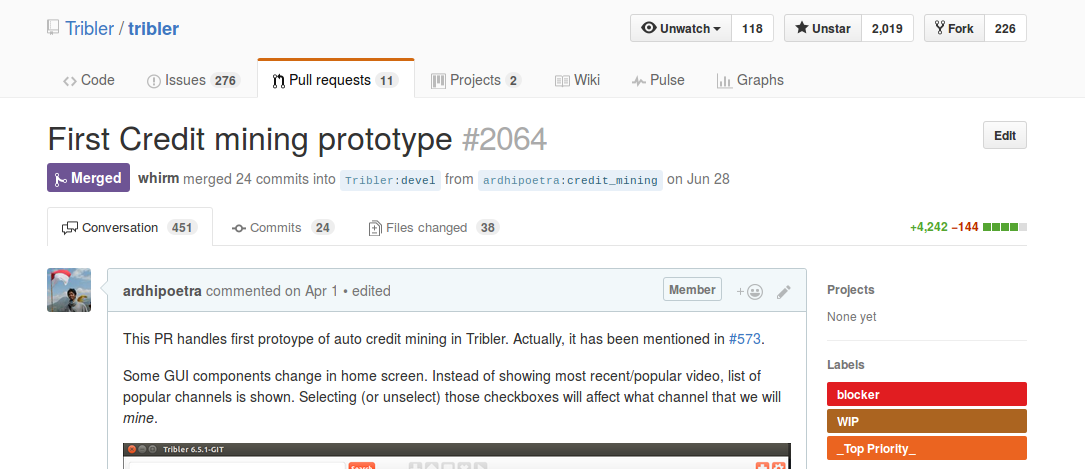
\includegraphics[width=\textwidth]{pics/cm_pr_crop.png}
	\caption[Merged pull request on credit mining prototype]{Merged pull request on credit mining prototype\footnotemark.}
	\label{fig:cmpullrequest}
\end{figure}
\footnotetext{Available in : \url{https://github.com/Tribler/tribler/pull/2064/}}

To ensure the quality of the main branch, any code submitted through a pull request is tested by a unit test mechanism. There are two categories in the credit mining unit tests. The first test checks its basic function such as policies, peer translation, RSS parser, similarity function, and mining configuration, along with its dependencies. It also tests for the unwanted/error case and how the credit mining system will react. The second test is more complex because it emulates the whole credit mining flow for each mining source type. For an RSS source, the test deploys a local server acting as an RSS feeder. As for a \textit{channel} source, the test suite prepares the environment by fabricating both local channel and torrent, inserting torrent metadata into the \textit{channel}, and pushing the created channel to \textit{AllChannelCommunity}. 

\subsection{Graphical user interface revampment}
\begin{figure}[h]
	\centering
	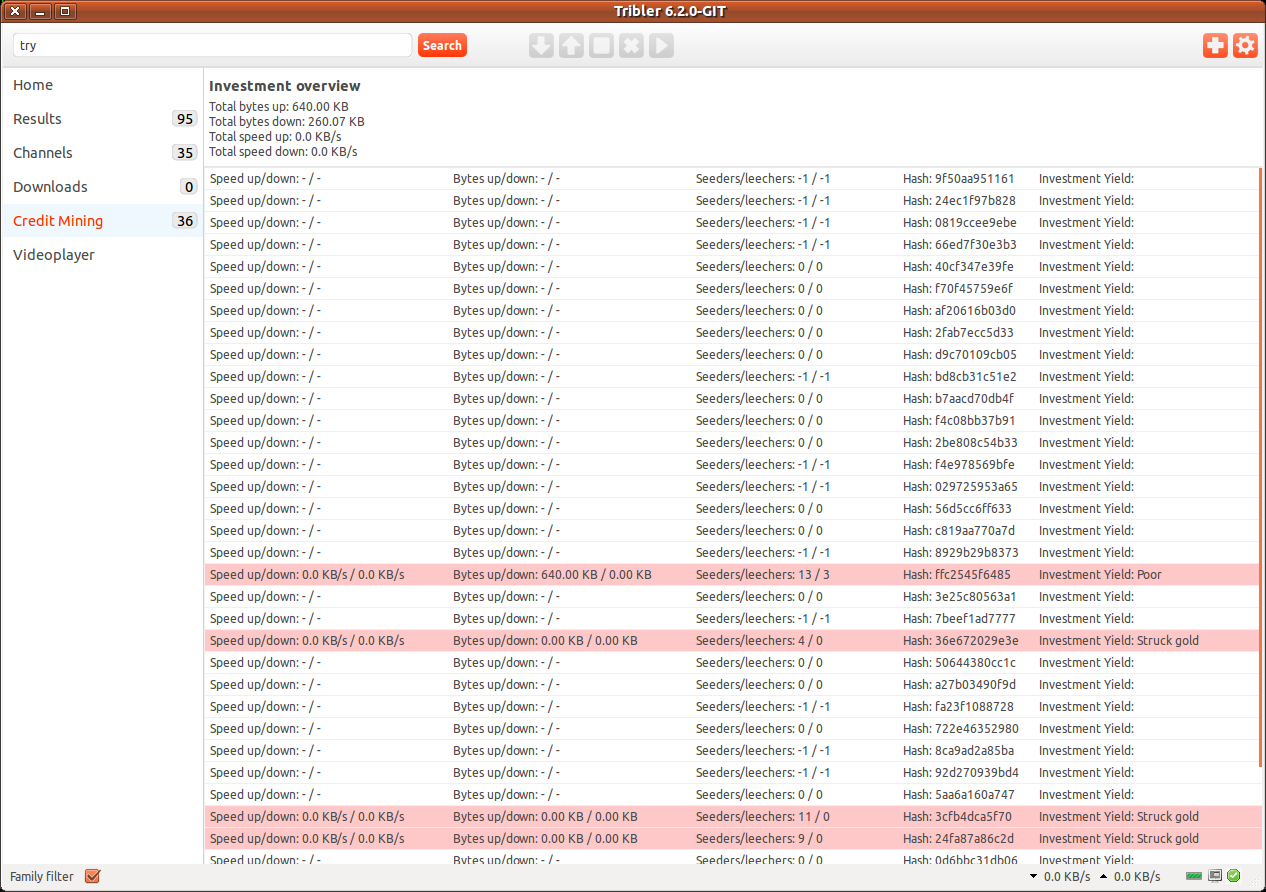
\includegraphics[width=0.8\textwidth]{pics/old_cm.png}
	\caption{The GUI for showing information from prior work \cite{2015:creditmining:capota}.}
	\label{fig:oldcm}
\end{figure}
In the prior version, it was not possible to add the mining sources except by changing the Tribler configuration file. There are also several limitations such as incompatible source and instability. Figure \ref{fig:oldcm} shows the only interface available from the previous work. As for our work, the credit mining main screen is shown in \ref{fig:overview}. We improved the investment summary by adding more mining source information. In the same window, we also integrated an interface to easily add or remove mining sources. Adding RSS and directory sources can be done by clicking the upper left option. This action will trigger a popup window like shown in Figure \ref{fig:overview}. Adding \textit{channel} as a source can be done by checking the boxes in the channel list.

\begin{figure}[h!]
	\begin{adjustwidth}{-1.5cm}{-1cm}
%		\begin{subfigure}[t]{0.8\textwidth}
			\centering
			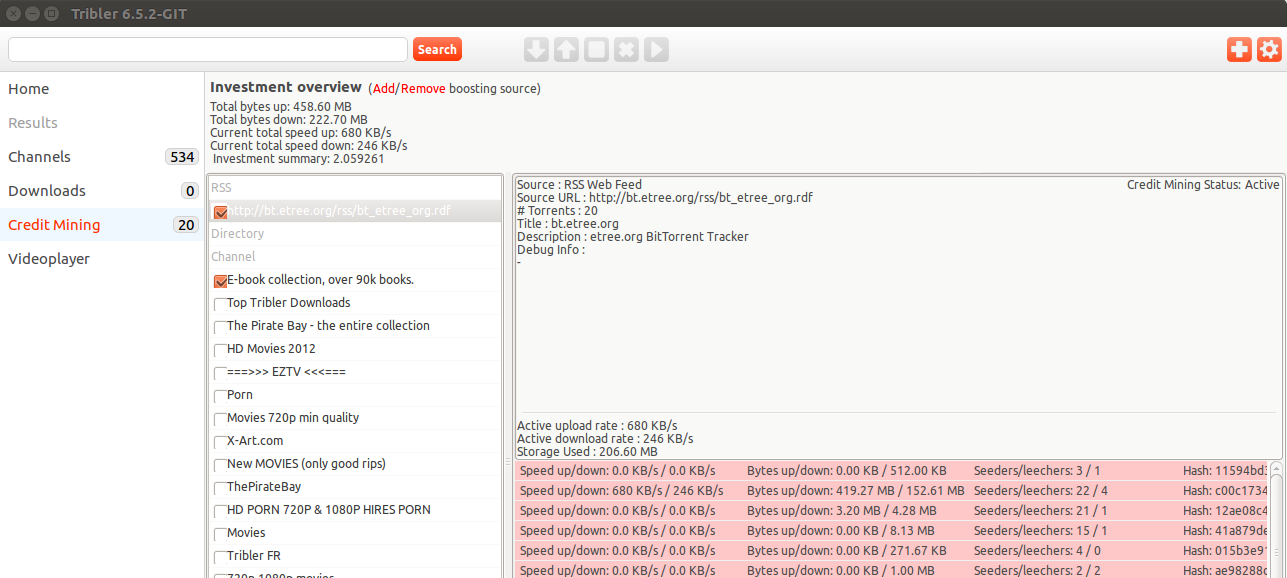
\includegraphics[width=1.2\textwidth]{pics/overview_result.png}
			\caption{Credit mining main window with adding new source.}
			\label{fig:overview}
%		\end{subfigure}
%		~
%		\begin{subfigure}[t]{0.6\textwidth}
%			\centering
%			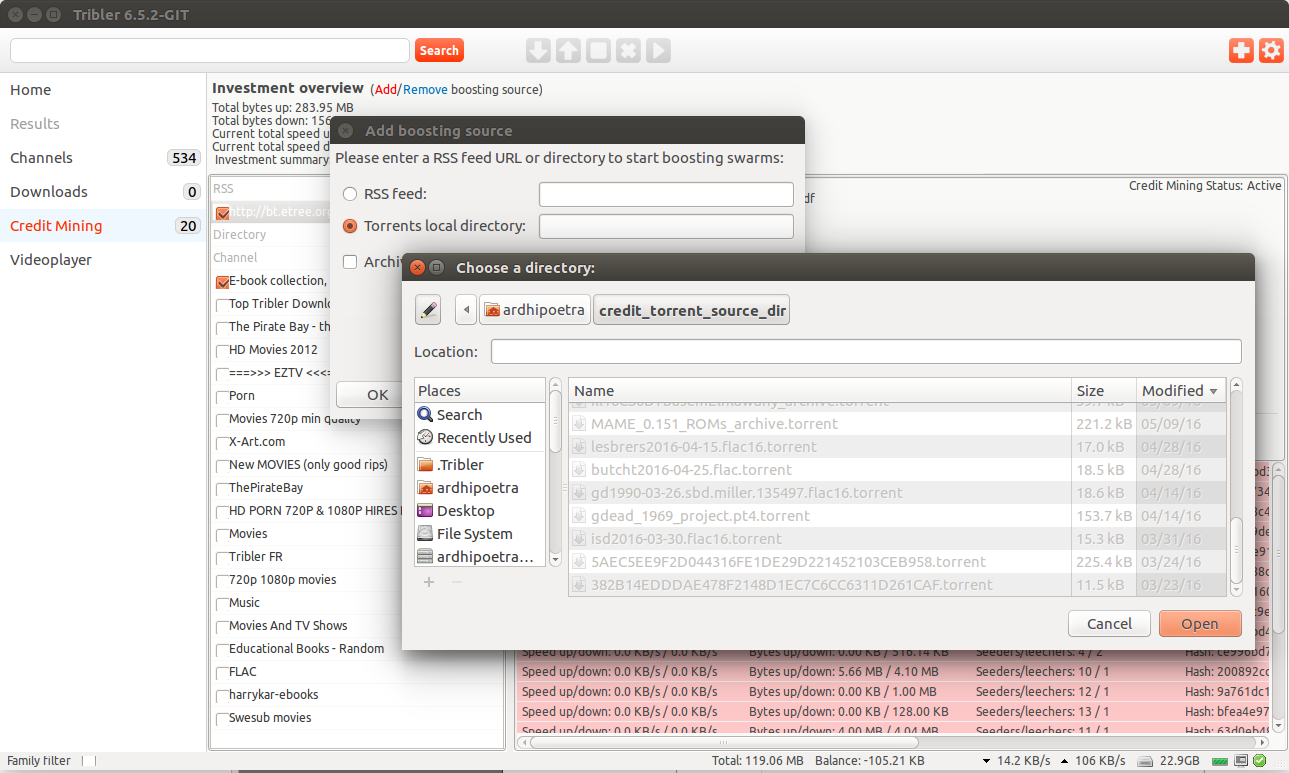
\includegraphics[width=\textwidth, height=6cm]{pics/add_source.png}
%			\caption{The interface of adding mining source.}
%			\label{fig:addsource}
%		\end{subfigure}
		
	\end{adjustwidth}
\end{figure}

As an experimental feature, the credit mining system is disabled by default in Tribler. Activating the credit mining module made the Tribler home screen change. We put several channels sorted by their popularity on the home screen, as shown in Figure \ref{fig:homecm}. The purpose is to encourage user to altruistically mine. To show the channel information, we provided two details. The first is the popularity, which is shown by the number of stars. The second is a random swarm that resides within a particular channel. A user can simply click on which channel they want to mine, either on this screen or the credit mining main screen. Both actions will also be reflected on the other screen. 

\begin{figure}[h]
	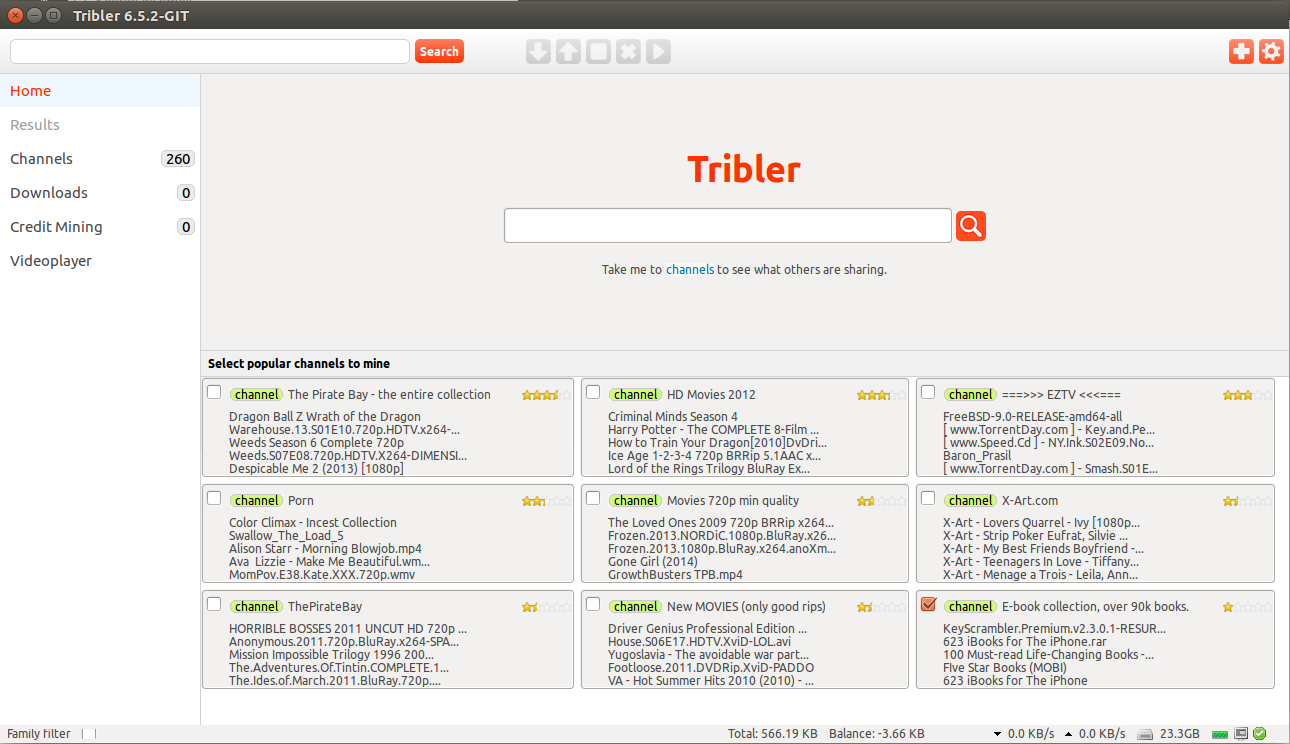
\includegraphics[width=\textwidth]{pics/home_channel.png}
	\caption{The home interface of Tribler with credit mining active.}
	\label{fig:homecm}
\end{figure}

%\todo[inline]{Add stuff}
\section{Gumby}
\label{section:gumby}
\textit{Gumby}\footnote{\url{https://github.com/Tribler/gumby}} is an experiment runner framework for both Tribler and Dispersy. Gumby can run on both local and cluster computer to emulate the experiment. Gumby runs on different scenarios, which consists of many commands, for each experiment. It also uses a configuration file to define all of the settings needed for running the experiment. The developer can easily specify the number of peers needed, the post-process script after running the experiment, the value that is needed to be distributed to all of the peers, and many other specifications. The most important part is to code the \textit{client} that is written in \texttt{python}. In the \textit{client} file, one must define how the experiment will run and behave, including the commands interpretation.

Gumby runs in a sequential manner with several steps as follows. First, gumby reads the scenario and configuration file. After deciding what type of experiment it has to run, it will clear the output directory. Moreover, in case gumby is running in cluster computer, it also need to synchronize the \textit{client} on multiple nodes. Next, the setup script will be executed. After that, gumby spawns Dispersy and the experiment tracker to monitor the nodes in case of error occurring. All of the experiment nodes communicate with the server using a specified IP address and port. Finally, both local and remote processes are started in parallel. Upon finishing the experiment, the server will wait for all node instances to exit and disconnect gracefully. Then it will copy the data to a predefined directory. Those data now can be processed using specified post-experiment script to generate items such as graphs and tables.

\subsection{Scenario and Configuration}
In gumby, it is not possible to intervene in the experiment on the fly. What the developer can do is specify commands in the scenario file. The scenario notation consists of the time of an action and the command itself. The specific node that needs to run the command can also be specified with curly brackets. Figure \ref{fig:gumbyscenario} shows the example of the gumby scenario. For example, command \texttt{@0:36 set\_boost\_settings boosting.ini.1 \{3\}} means in seconds 36, gumby will run command \texttt{set\_boost\_settings} with \texttt{boosting.ini.1} as a parameter on node number 3. 

\begin{verbbox}
@0:0 set_master_member 3081a73010...e75
@0:2 start_dispersy {1-3}
@0:10 start_session
@0:22 online
@0:23 set_speed 0 0 {3}
@0:32 create {1}
@0:35 publish file1gb_1 1524288077 {1}
@0:36 set_boost_settings boosting.ini.1 {3}
@0:37 start_boosting {3}
@0:40 add_source http://bt.etree.org/rss/bt_etree_org.rdf {3}
@1:15 start_download file1gb_1 {2}
@1:33 reset_dispersy_statistics
@0:43100 stop
\end{verbbox}

\begin{figure}[h]
	\fbox{\theverbbox}
	\caption{Scenario format example}
	\label{fig:gumbyscenario}
\end{figure}

In contrast to the scenario file, the gumby configuration file only contains variables that need to be filled. These variables can be accessed from inside the \textit{client}. Figure \ref{fig:gumbyconf} shows an example of configuration format in gumby. There are some necessary variables such as the experiment name and \texttt{tracker\_cmd}. Some of the variables are required by specific conditions. For example, if variable \texttt{local\_instance\_cmd} is \texttt{'das4\_reserve\_and\_run.sh'}, it is necessary to call the other 4 sub-variables that are recognized by \texttt{das4\_} precedence. There are also variables that are completely optional. In this case, specifying variable \texttt{scenario\_file} is optional to point which scenario gumby need to run.

\begin{verbbox}
experiment_name = "CreditRunner_base_DAS"
experiment_server_cmd = 'experiment_server.py'

local_setup_cmd = 'das4_setup.sh'
local_instance_cmd = 'das4_reserve_and_run.sh'

output_dir = '/var/scratch/aputra/cmining'

das4_node_amount = 2
das4_node_timeout = 3600
das4_instances_to_run = 5
das4_node_command = "creditmining.py"

tracker_cmd = 'run_tracker.sh'

use_local_venv = True

scenario_file = "creditmining_base.scenario"
post_process_cmd = "gumby/scripts/post_credit_mining.sh"
\end{verbbox}

\begin{figure}[h!]
	\fbox{\theverbbox}
	\caption{Configuration format example}
	\label{fig:gumbyconf}
\end{figure}

\section{Experimental setup}
\label{section:cmexp}
We now focus on what setup the credit mining system will be evaluated. In general, there are two aspects we want to address. The first one is how the credit mining system can gain benefit for its user. This means that a user is expected to get a considerable amount of credit with a relatively small investment. The second aspect is to find out how the credit mining system can benefit the swarms as a whole. This can be done by monitoring the performance of each of the peers. If each of the peers' performance is increasing, then the swarm itself has its capacity increased as well.

%\begin{table}[h]
%	\centering
%	\caption{Experiment scheme}
%	\label{tbl:expswarmperf}
%	\begin{tabular}{|c|c|c|c|c|c|}
%		\hline
%		\textbf{300mb} & \textbf{1gb\_1} & \textbf{1gb\_2} & \textbf{5gb} & \textbf{Total peers} & \textbf{Event} \\ \hline
%		0 & 0 & 0 & 0 & 1 & Publisher \\ \hline
%		4 & 5 & 2 & 8 & 19 & Seeders \\ \hline
%		10 & 5 & 10 & 3 & 28 & Wave 1 \\ \hline
%		4 & 1 & 5 & 8 & 18 & Wave 2 \\ \hline
%		7 & 10 & 10 & 7 & 34 & Wave 3 \\ \hline
%		0 & 0 & 0 & 5 & 5 & 30min-1 \\ \hline
%		0 & 0 & 5 & 0 & 5 & 30min-2 \\ \hline
%		0 & 5 & 0 & 0 & 5 & 30min-3 \\ \hline
%		5 & 0 & 0 & 0 & 5 & 30min-4 \\ \hline
%		\hline
%		30 & 26 & 32 & 31 & 120 & \textbf{Total Peers} \\ \hline
%	\end{tabular}
%\end{table}

\subsection{Experiment conditioning}
The experiments were conducted in different scenarios and architectures. We handcrafted the environment needed for all of the experiments. In this thesis, all of the scenarios are presented in the appendix. Most of the experiments are conducted in a closed environment using \textit{channel} as dissemination method. A swarm with fabricated files as content is created. This swarm is then inserted into a particular \textit{Channel}. This \textit{channel} can be accessed from all the nodes using Dispersy. In the end, the user can get the metadata of this swarm such as files list, infohash, and other information typically found in the \texttt{.torrent} file. To be able to compare the system performance to prior work, we used etree.org (\url{http://bt.etree.org/rss/bt_etree_org.rdf}) as a mining source. This is because the prior work's system is not compatible with gumby. Etree.org is a legal community that shares music with permission from authors. This community is relatively active, and newly published swarms usually have sufficient supply and demand for testing. 

We have two different sites to accommodate our experiment. First is DAS-4\footnote{\url{http://www.cs.vu.nl/das4}} (The Distributed ASCI Supercomputer 4) cluster which runs the CentOS Linux operating system. DAS-4 nodes have a dual quad-core processor with 24 GB memory. The interconnection speed between nodes is 1Gbit/s. The DAS site is used to run experiments that need many peers in a closed environment. It has \textit{libtorrent} version 1.1.1 installed. The second site is the local computer named DUTIJC running Arch Linux with \textit{libtorrent} version 1.0.10. This site has 6 GB memory and quad-core \textit{i7-920} processor. The DUTIJC site is used for running long experiments. 

In our controlled environment, a node can be categorized as publisher, seeder, downloader, or credit miner. A single node will act as a \textit{publisher} of this swarm. It creates a \textit{channel} and fabricated files, generates metadata, pushes it into the \textit{channel}, and seeds for the rest of the experiment. Another node can help become a \textit{seeder} for the swarm if necessary. For other nodes, it can be either download or can activate the credit mining system. This \textit{channel} can be added to the credit mining system as a mining source. As for \textit{downloaders}, they can both start and stop downloading from a swarm identified by its name. 

%\subsection{Comparing performance}
%One checkpoint of this work is comparing the performance of each of the experiments. In the prior work by \citeauthor{2015:creditmining:capota}, they used \textit{net upload gain} as a parameter to measure how many credit user already gain. Net upload gain is a difference between uploaded and downloaded bytes. Moreover, to measure the efficiency of credit mining system, they also defined \textit{normalized upload gain} which is the ratio between \textit{net upload gain} and total downloaded bytes.
%
%\todo[inline]{add other metric to compare}

\subsection{Code modification for experiments}
\label{section:predlsetup}
In this section, we want to focus on the assumption and code modification for the experiment in a closed environment. As we limit the download and upload rate, we assume the system knows this limit. This makes, for example, finding leftover bandwidth trivial. We also defined the multiplier in scoring policy. The value of $M\_leech$, $M\_pratio$, $M\_avail$ are 5, 3, and 4, respectively. The reason behind this number is as follows. We intend to make all multipliers relatively equal and small. However, it is important to distinguish the features of the policy. The difference between multipliers should not be so significant, for example as twice as much as another. $M\_leech$ and $M\_avail$ show the performance shortage in swarms. $M\_leech$ is used in previous work, so it has a bigger multiplier than $M\_avail$. $M\_pratio$ is a tie-breaker, thus assigned the smallest multiplier.

We then altered the code on three occasions. Firstly, the system will aggressively connect to each other in a closed environment. The IP address and port for each node are determined prior to launch. We use this information to build full mesh connection topology. Secondly, any peer information outside the predetermined range is rejected. The third alteration is only applied in the \textit{prospecting} experiment. In this experiment, we increase the maximum swarm per source to one hundred, and set the number of active swarm to zero. Moreover, after a swarm has been \textit{prospected}, instead of sending it to miners, we retrieve the information and then delete it afterward. By this approach, the swarm per source slot will be freed faster, and the experiment results will still be valid. 

\subsubsection{Torrent crawler}
For the \textit{prospecting} experiment to succeed, a large number of swarms are needed. Although many swarms can be retrieved from anywhere including illegal sources, we want to contribute to the society by providing support for the legal ones. We implemented a legal torrent crawler that can be accessed at \url{https://github.com/ardhipoetra/legal-torrent-crawler}. It uses \textit{scrapy}\footnote{\url{https://scrapy.org/}} as a scraper for the torrent portal sites. The crawler will access these sites, find any link to \texttt{.torrent} file, then download and categorize it. So far, we have implemented the crawler for 8 sites as shown in Table \ref{tbl:legaltorrentsource}. The crawler is completely unrelated from the credit mining system. It can be executed independently. The crawler is executed before the \textit{prospecting} experiment is started. The output of this crawler is a collection of \texttt{.torrent} files in a single directory which act as the input for the prospecting experiment.

\begin{table}[h]
	\centering
	\caption{Legal torrent source.}
	\label{tbl:legaltorrentsource}
	\begin{tabular}{lp{8.5cm}}
		\hline
		Source & Description \\ \hline
		\url{etree.org} & Live music trading community. \\
		\url{legittorrents.info} & Self-moderated torrent tracker and portal. \\
		\url{librivox.org} & Public domain audiobooks read by volunteers. \\
		\url{linuxtracker.org} & Linux distro torrent aggregator. \\
		\url{distrowatch.com} & Linux distro torrent aggregator. \\
		\url{mininova.org} & Torrent directory site. Used to host copyrighted material but now is no more.\\
		\url{sxswtorrent.com} & Sample music sharing on SXSW events. \\
		\url{vodo.net} & Media distributor. Offers legal films, books, and music.
	\end{tabular}
\end{table}

%\subsection{Experiment scenarios}
%\begin{enumerate}
%	\item simple closed var:policy, num, stimulate
%	\item prior work comparison
%	\item predownload. var:policy
%	\item user activity. 
%	\item many simple-closed. var. num. stimulate
%\end{enumerate}
%
%\subsection{Parameter for evaluation}
\chapter{Performance Evaluation}
\label{chp:perfeval}

Bottleneck can happen in the early time of share mode. The combination of line \ref{alg:l_lts:retdlenough} and \ref{alg:l_lts:retdling} will hold downloading any piece if the uploaded amount is not enough based on the piece we have. Let say we already which piece to download from line \ref{alg:l_lts:dlrare}. In the next round, this piece is not rare anymore. Therefore, we cannot upload this piece. 

\section{Predownload}
\begin{figure}[h]
	\centering
	\includegraphics[width=\textwidth]{pics/results/dpredown_t30i30.pdf}
	\caption{Predownload success percentage}
	\label{fig:predownprecent}
\end{figure}

\begin{figure}[h]
	\centering
	\includegraphics[width=\textwidth]{pics/results/hpredown_t30i30.pdf}
	\caption{Predownload distributed time}
	\label{fig:predownhist}
\end{figure}

\begin{figure}[h]
	\centering
	\includegraphics[width=\textwidth]{pics/results/ppredown_t30i30.pdf}
	\caption{Amount of peer discovered}
	\label{fig:peeramount}
\end{figure}
\todo{From experiment \#46 500 swarm in source. 12h}
\subsection{Other piece selection}
Random : some of the piece start downloading near the end, so it can't be decided in which distribution.

Seq : 1 swarm also

\begin{figure}[h]
	\centering
	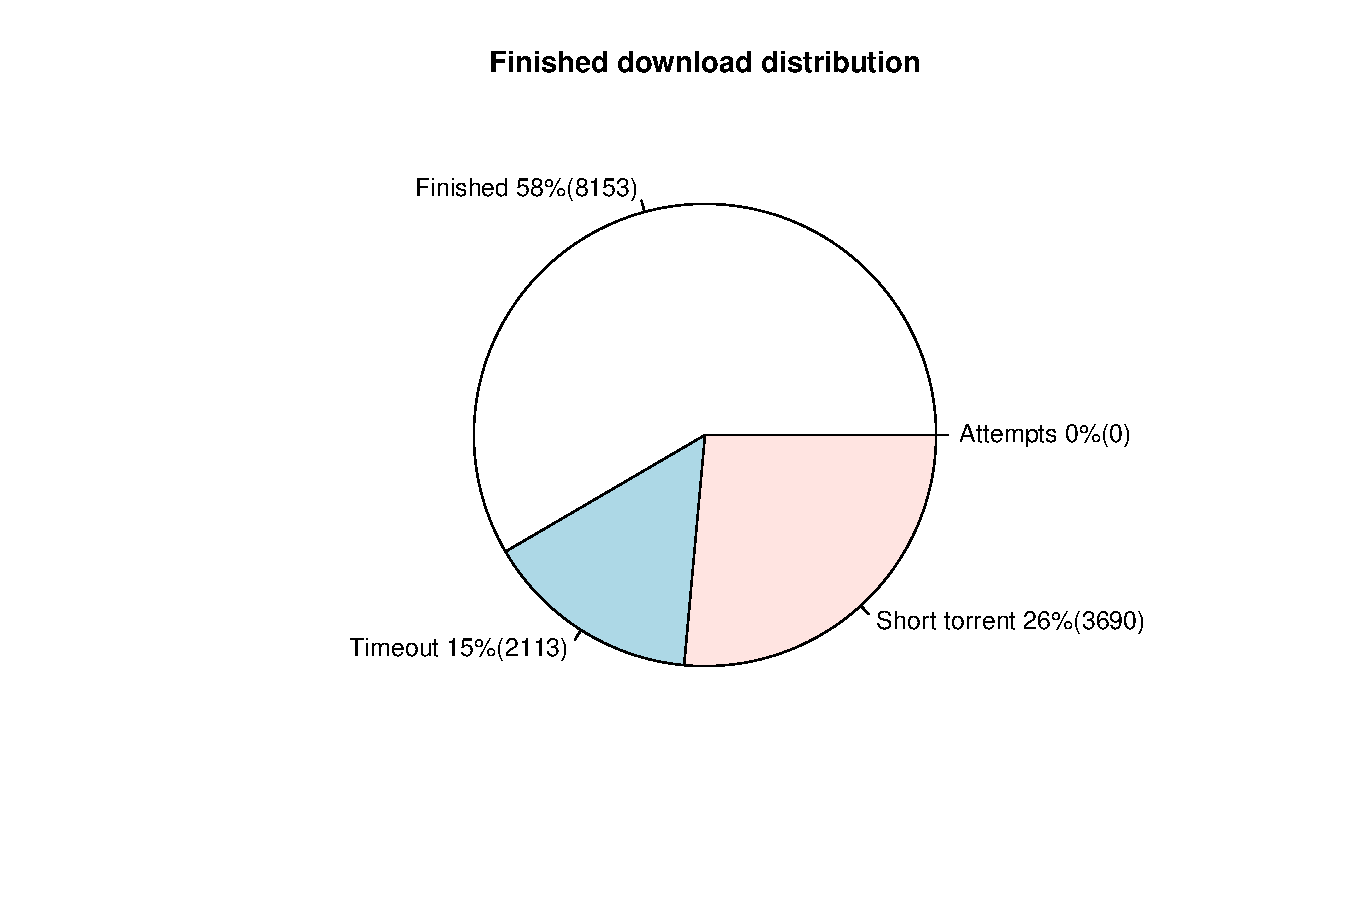
\includegraphics[width=\textwidth]{pics/results/dpredown_random.pdf}
	\caption{Predownload success percentage in random piece selection}
	\label{fig:predownprandom}
\end{figure}

\begin{figure}[h]
	\centering
	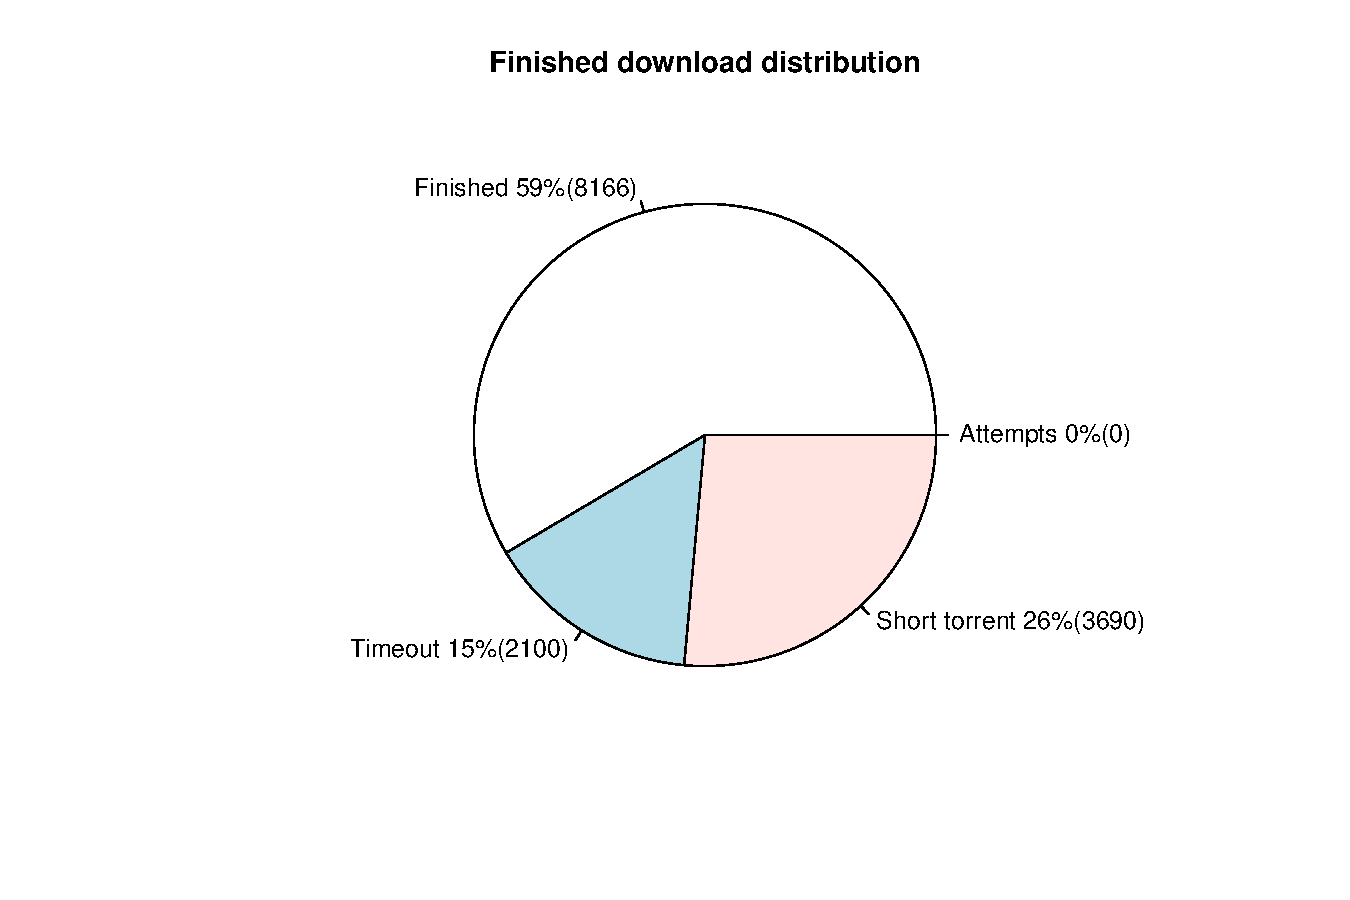
\includegraphics[width=\textwidth]{pics/results/dpredown_sequential.pdf}
	\caption{Predownload success percentage in sequential piece selection}
	\label{fig:predownpseq}
\end{figure}
\clearpage
% 100 swarm for 12, 24. 500 swarm for 24h
\section{Comparison vs old}
\begin{figure}[h]
	\begin{adjustwidth}{-2.5cm}{}
		\begin{subfigure}[t]{0.7\textwidth}
			\centering
			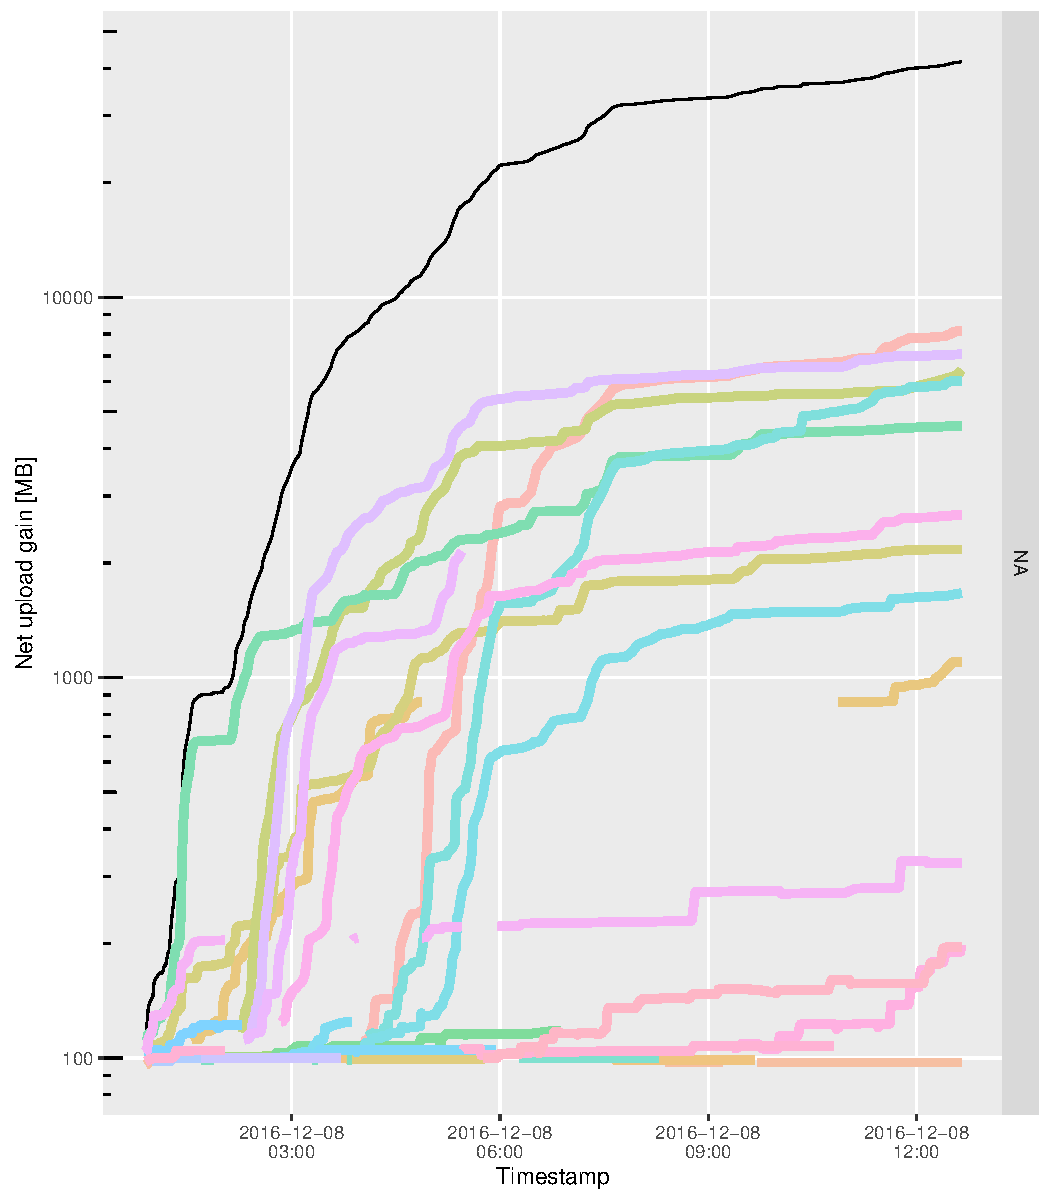
\includegraphics[width=\textwidth]{pics/results/b133.pdf}
			\caption{12 hour new experiment.}
		\end{subfigure}
		~
		\begin{subfigure}[t]{0.7\textwidth}
			\centering
			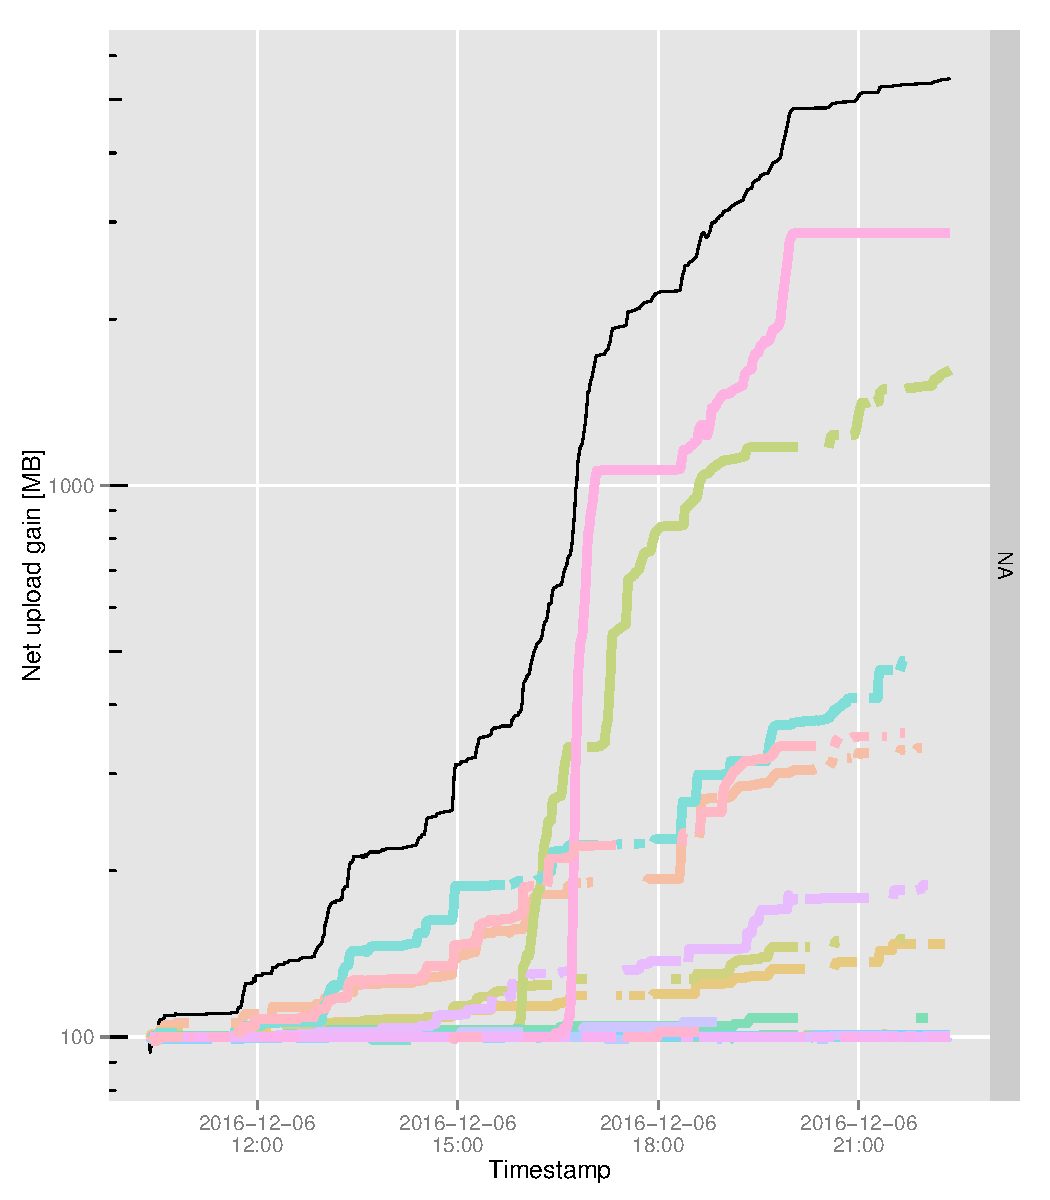
\includegraphics[width=\textwidth]{pics/results/m136.pdf}
			\caption{12 hour old experiment}
		\end{subfigure}
		\caption{New vs old experiments (run separately) result on 12 hour}
	\end{adjustwidth}
\end{figure}

\begin{figure}[h]
		\begin{adjustwidth}{-2.5cm}{}
	\begin{subfigure}[t]{0.7\textwidth}
		\centering
		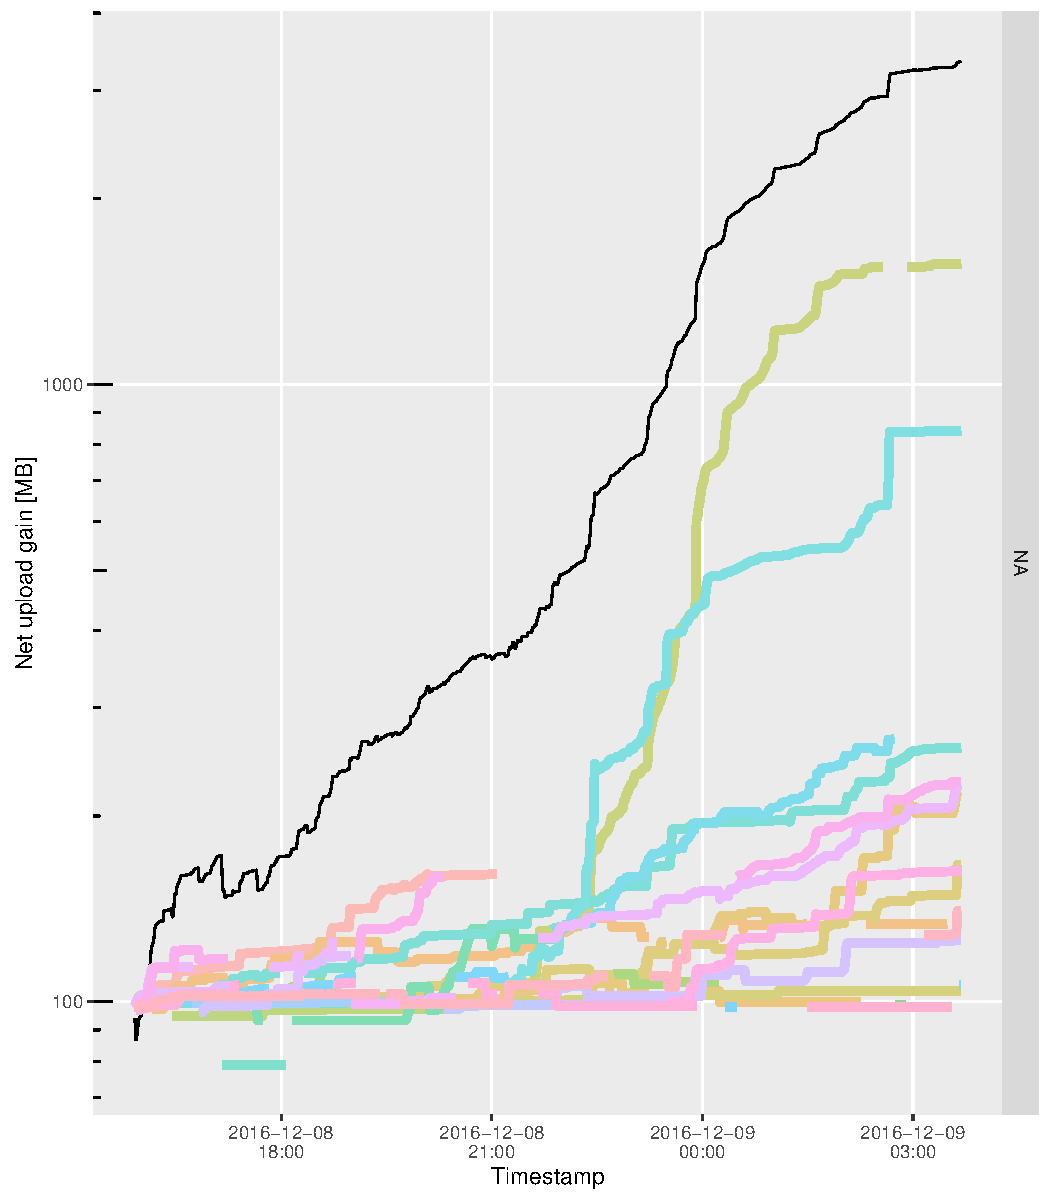
\includegraphics[width=\textwidth]{pics/results/b134.pdf}
		\caption{12 hour new experiment.}
	\end{subfigure}
	~
	\begin{subfigure}[t]{0.7\textwidth}
		\centering
		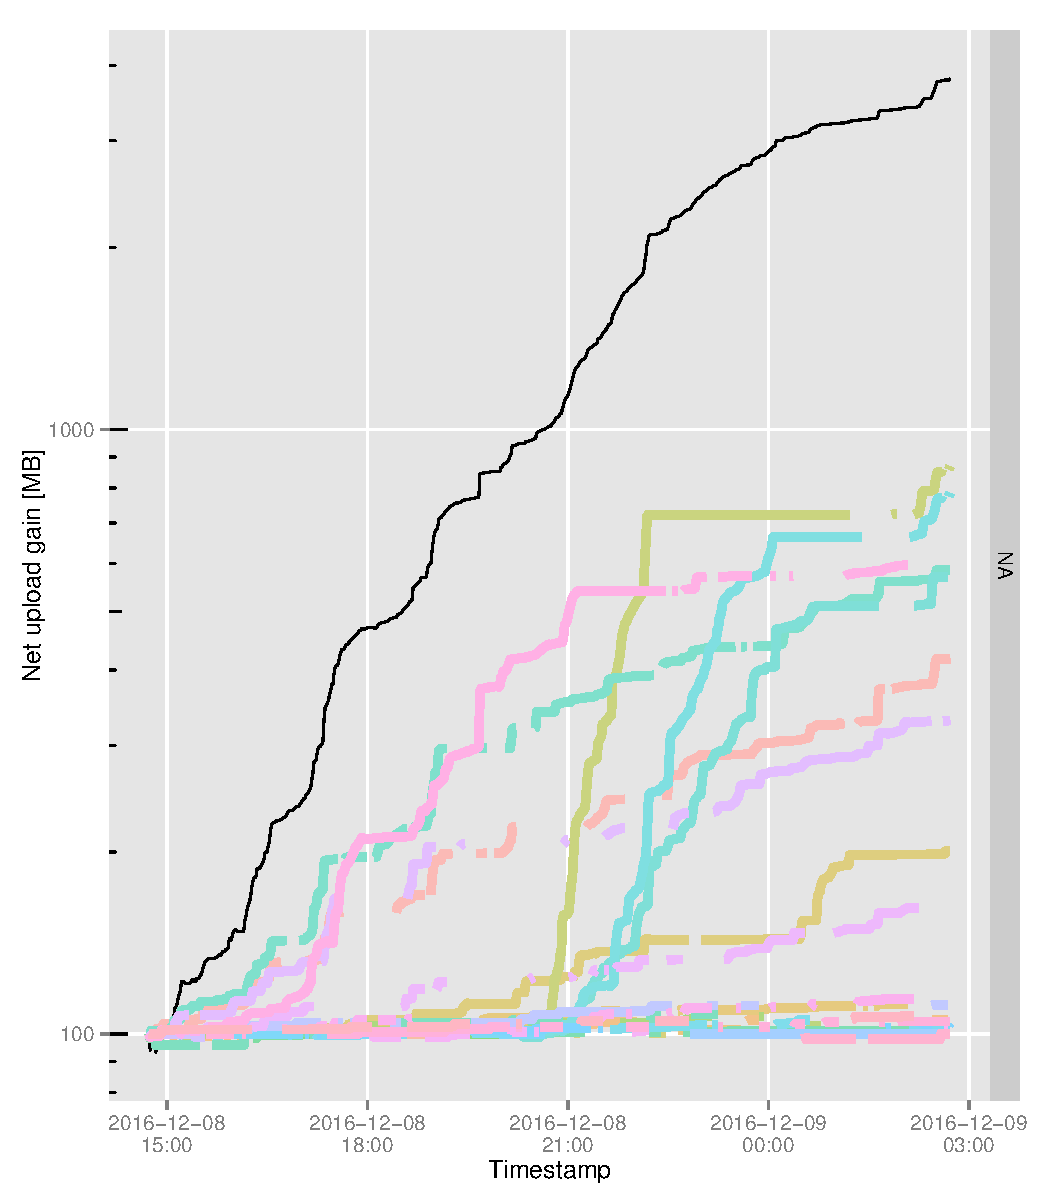
\includegraphics[width=\textwidth]{pics/results/m137.pdf}
		\caption{12 hour old experiment}
	\end{subfigure}
	\caption{New vs old experiments (run in parallel) result on 12 hour}
		\end{adjustwidth}
\end{figure}

\begin{figure}[h!]
	\begin{adjustwidth}{-2.5cm}{}
		\begin{subfigure}[t]{0.7\textwidth}
			\centering
			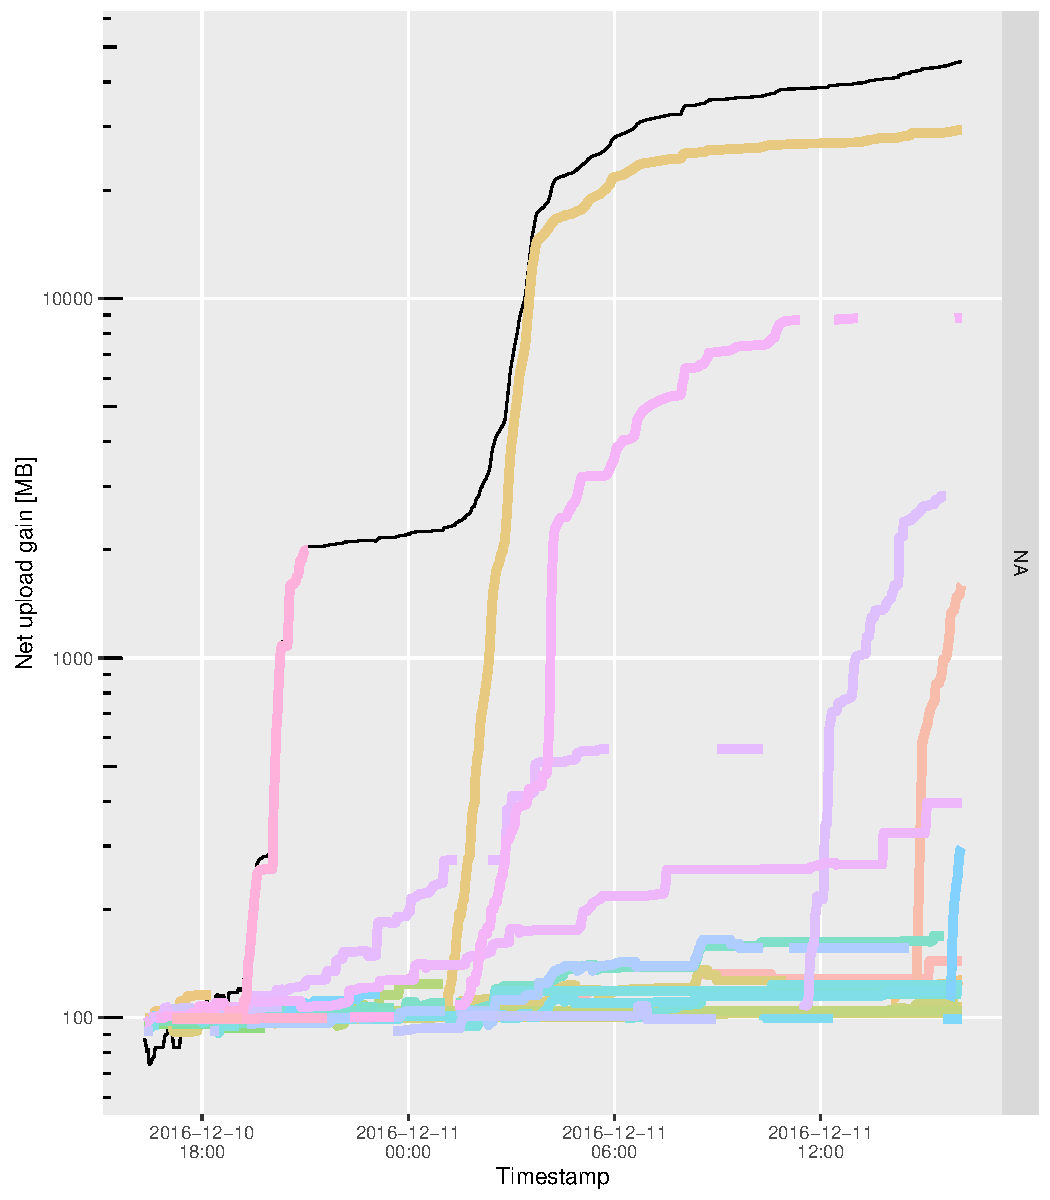
\includegraphics[width=\textwidth]{pics/results/b136.pdf}
			\caption{24 hour new experiment.}
		\end{subfigure}
		~
		\begin{subfigure}[t]{0.7\textwidth}
			\centering
			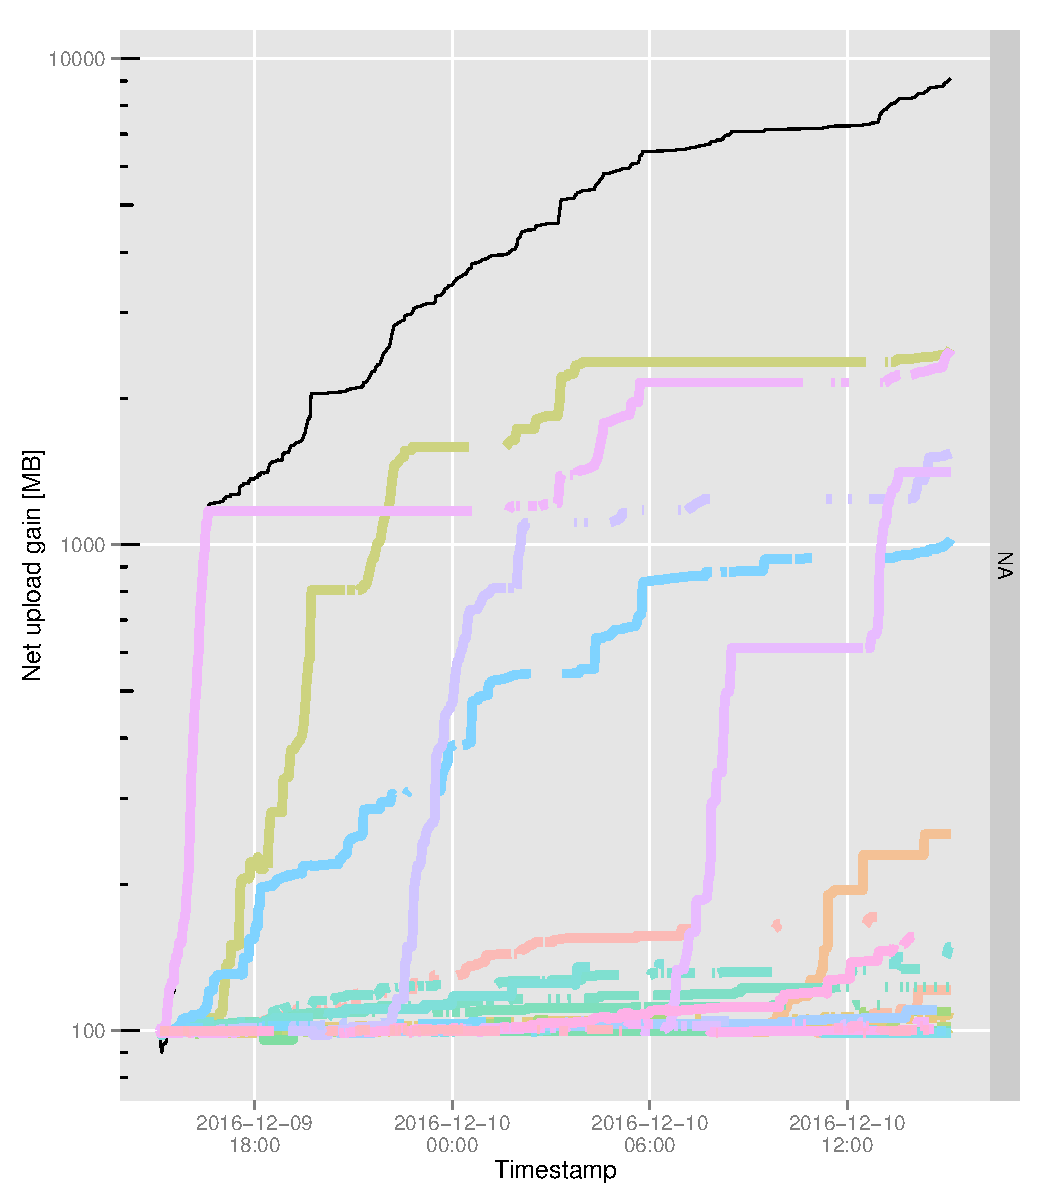
\includegraphics[width=\textwidth]{pics/results/m138.pdf}
			\caption{24 hour old experiment}
		\end{subfigure}
		\caption{New vs old experiments (run separately) result on 24 hour}
	\end{adjustwidth}
\end{figure}

\begin{figure}[h!]
	\begin{adjustwidth}{-2.5cm}{}
		\begin{subfigure}[t]{0.7\textwidth}
			\centering
			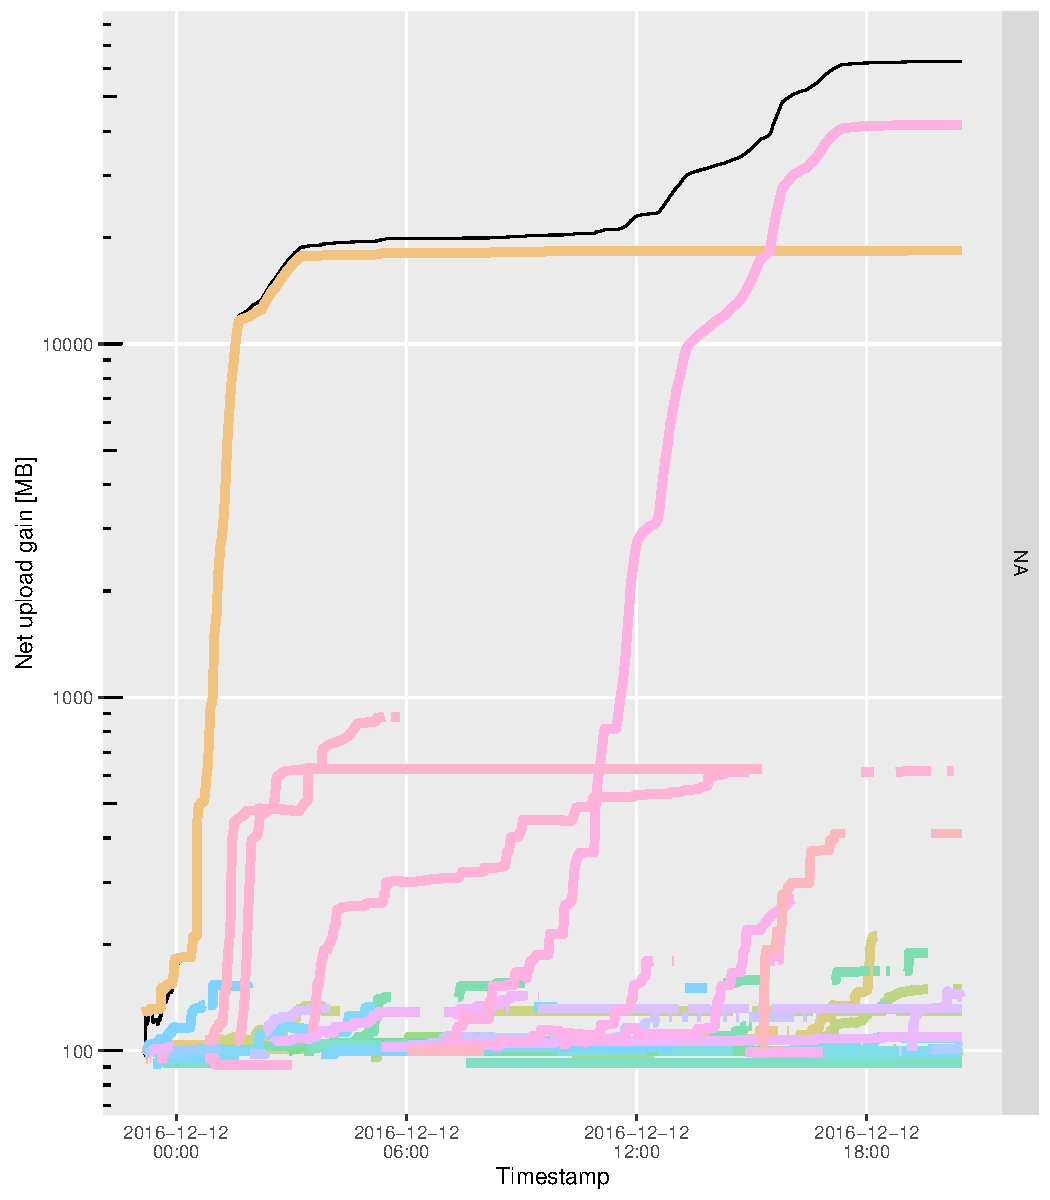
\includegraphics[width=\textwidth]{pics/results/b137.pdf}
			\caption{24 hour new experiment.}
		\end{subfigure}
		~
		\begin{subfigure}[t]{0.7\textwidth}
			\centering
			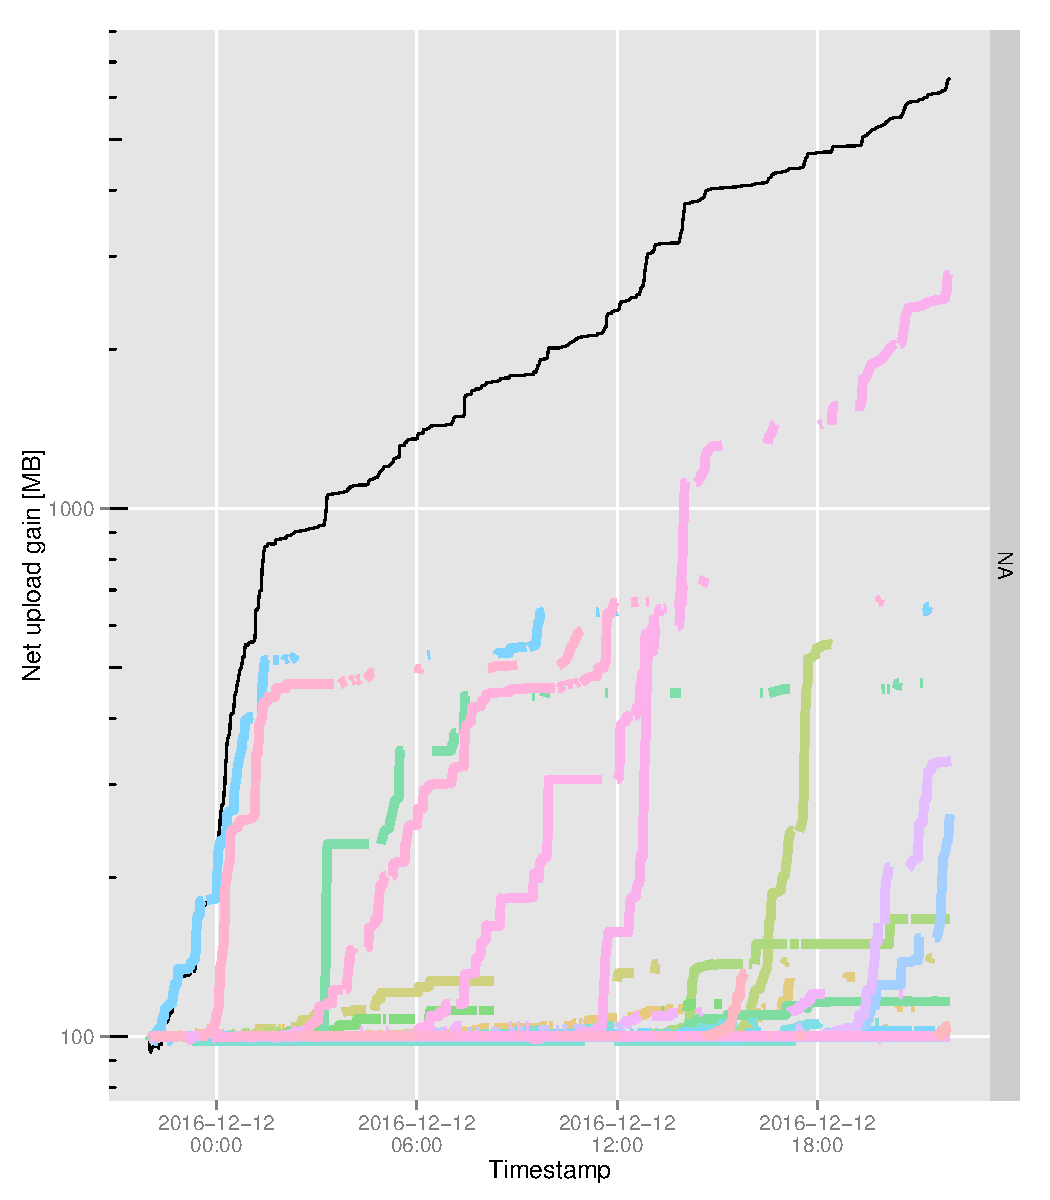
\includegraphics[width=\textwidth]{pics/results/m139.pdf}
			\caption{24 hour old experiment}
		\end{subfigure}
		\caption{New vs old experiments (run in parallel) result on 24 hour}
	\end{adjustwidth}
\end{figure}
%\begin{itemize}
%	\item old one use \textit{net upload gain}. etree.org for two day (48 hour). Test with 1 and half day.
%	\item Best old one is SeederRatio with 5 minute with 1 ratio (gain higher upload gain). Optimal : 3 ratio.
%	\item CM+boost : seederratio, 5 minutes, 3 ratio
%	\item mihai 136 12 hour. runs first. 6dec
%	\item cm 133. 12 hour. runs second. 8dec
%	\item mihai 137, cm 134 : 12 hour. In parallel
%	\item mihai 138 -> cm 136 24h
%	\item mihai 139 & 137 24h par
%\end{itemize}
\clearpage
\section{Priority}
\todo[inline]{WORK ON PROGRESS - Run experiment to find out}
% #50 -> 25k secs : 7 hour
% #50 -> 12h : 
\todo[inline]{temporary graph}
\begin{figure}[h]
	\centering
	\includegraphics[width=\textwidth]{pics/results/tmp_prio_4.png}
	\caption{Download speed of user download activity vs credit mining}
	\label{fig:cmpriomeanagg}
\end{figure}
\begin{figure}[h]
	\centering
	\includegraphics[width=\textwidth]{pics/results/tmp_prio_5.png}
	\caption{Download speed of user download activity only}
	\label{fig:cmpriomean}
\end{figure}

\clearpage
\section{Swarm performance}
\todo[inline]{WORK ON PROGRESS - Waiting for results}
\begin{figure}[h]
	\centering
	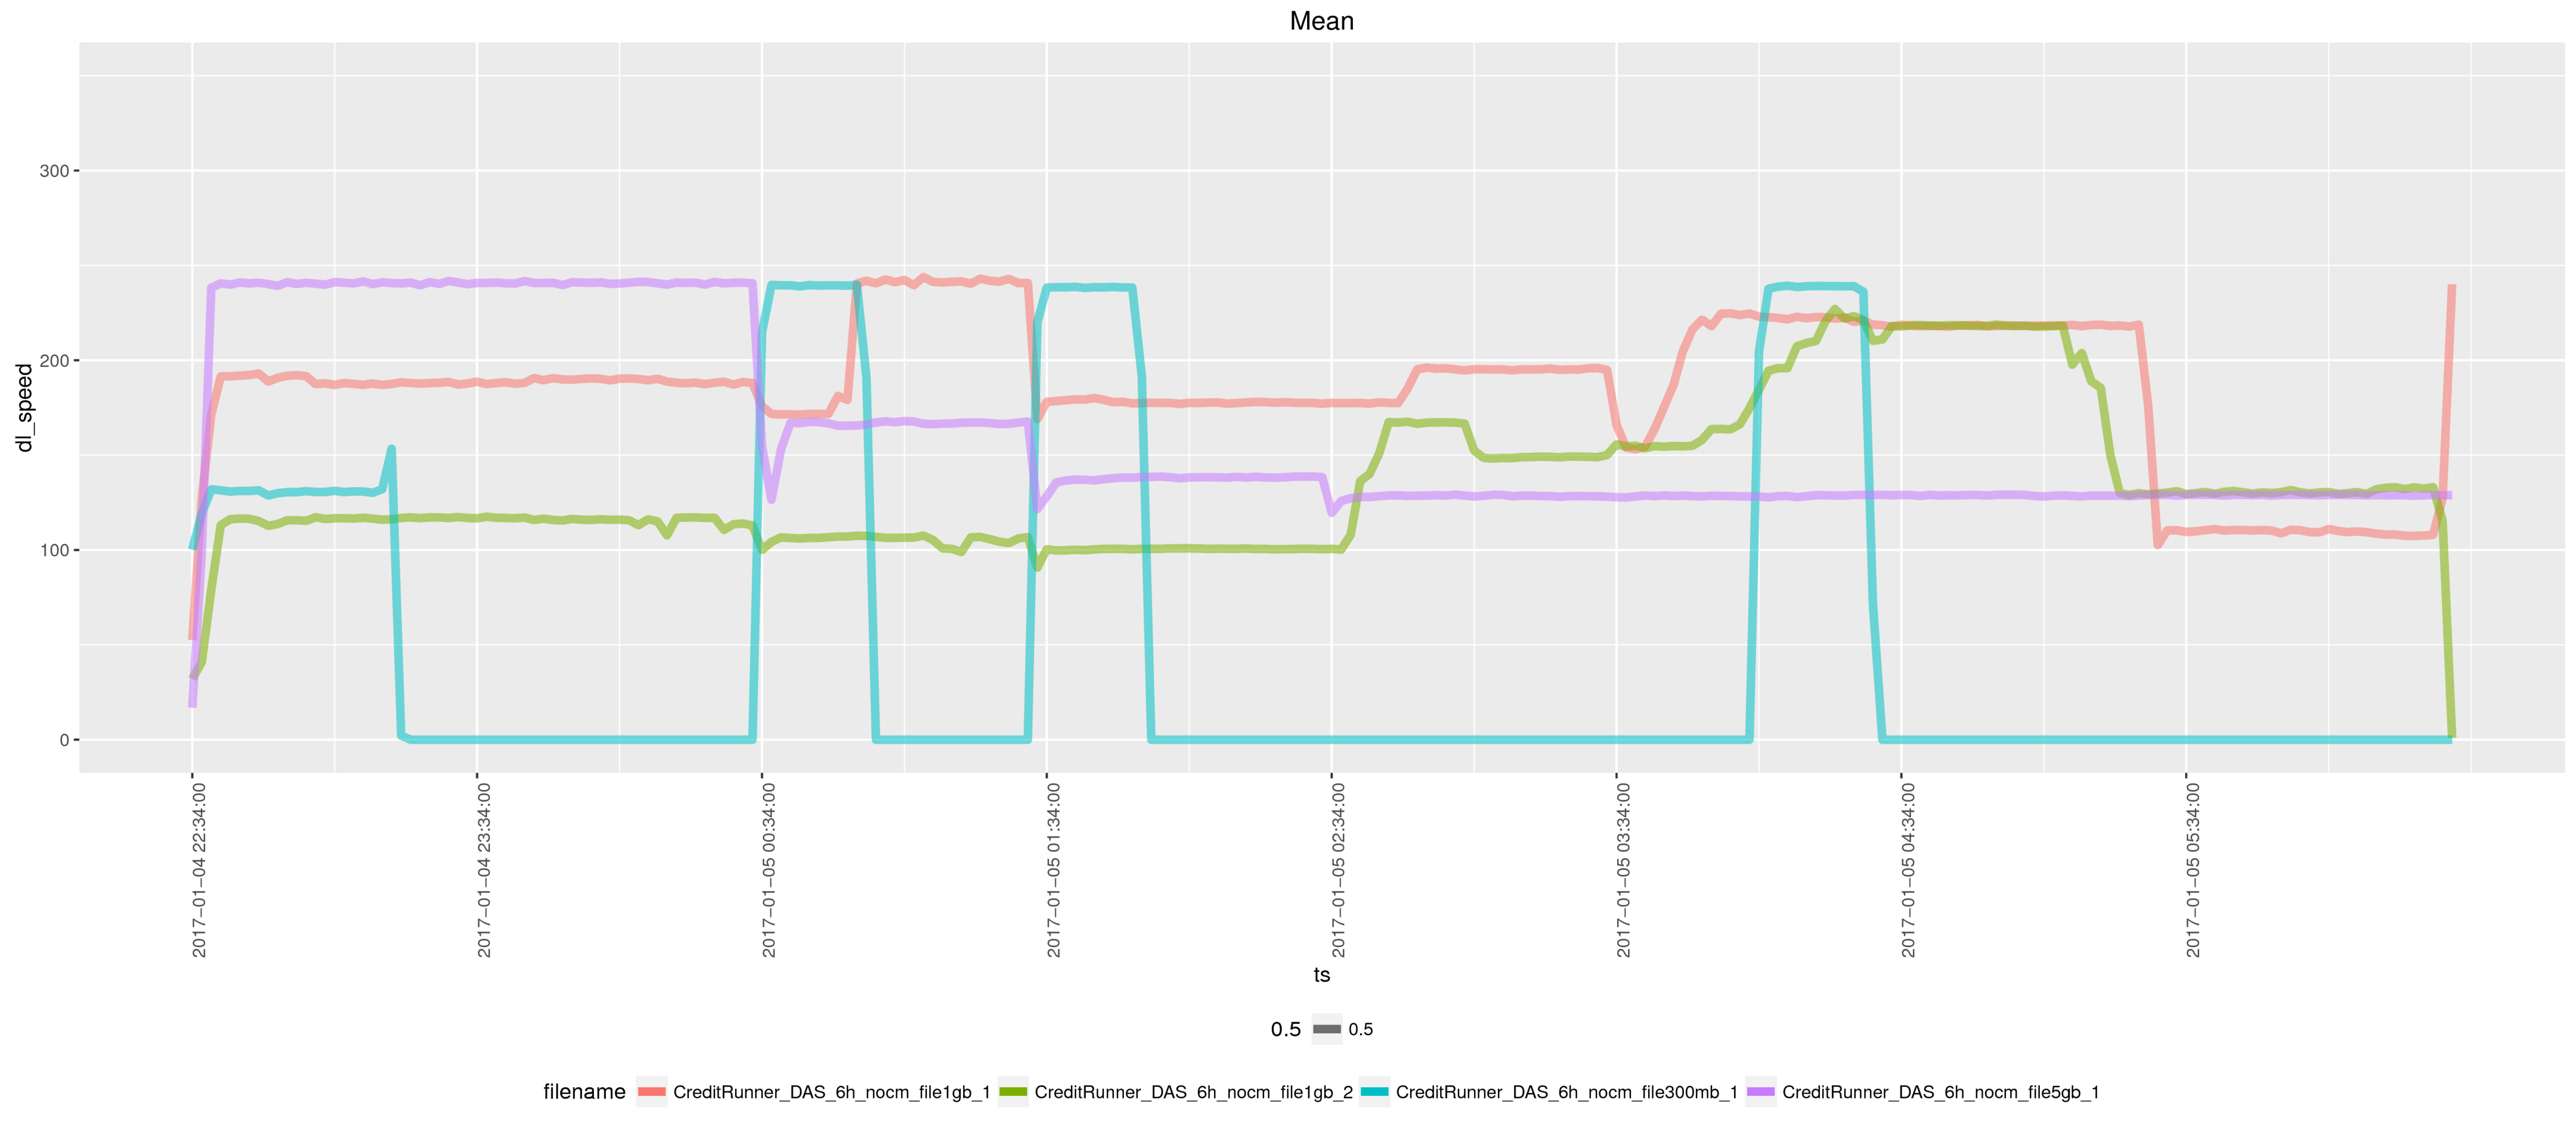
\includegraphics[width=\textwidth]{pics/results/reg_nocm.png}
	\caption{Swarm performance without credit mining}
	\label{fig:swarmnocmperf}
\end{figure}

\begin{figure}[h]
	\centering
	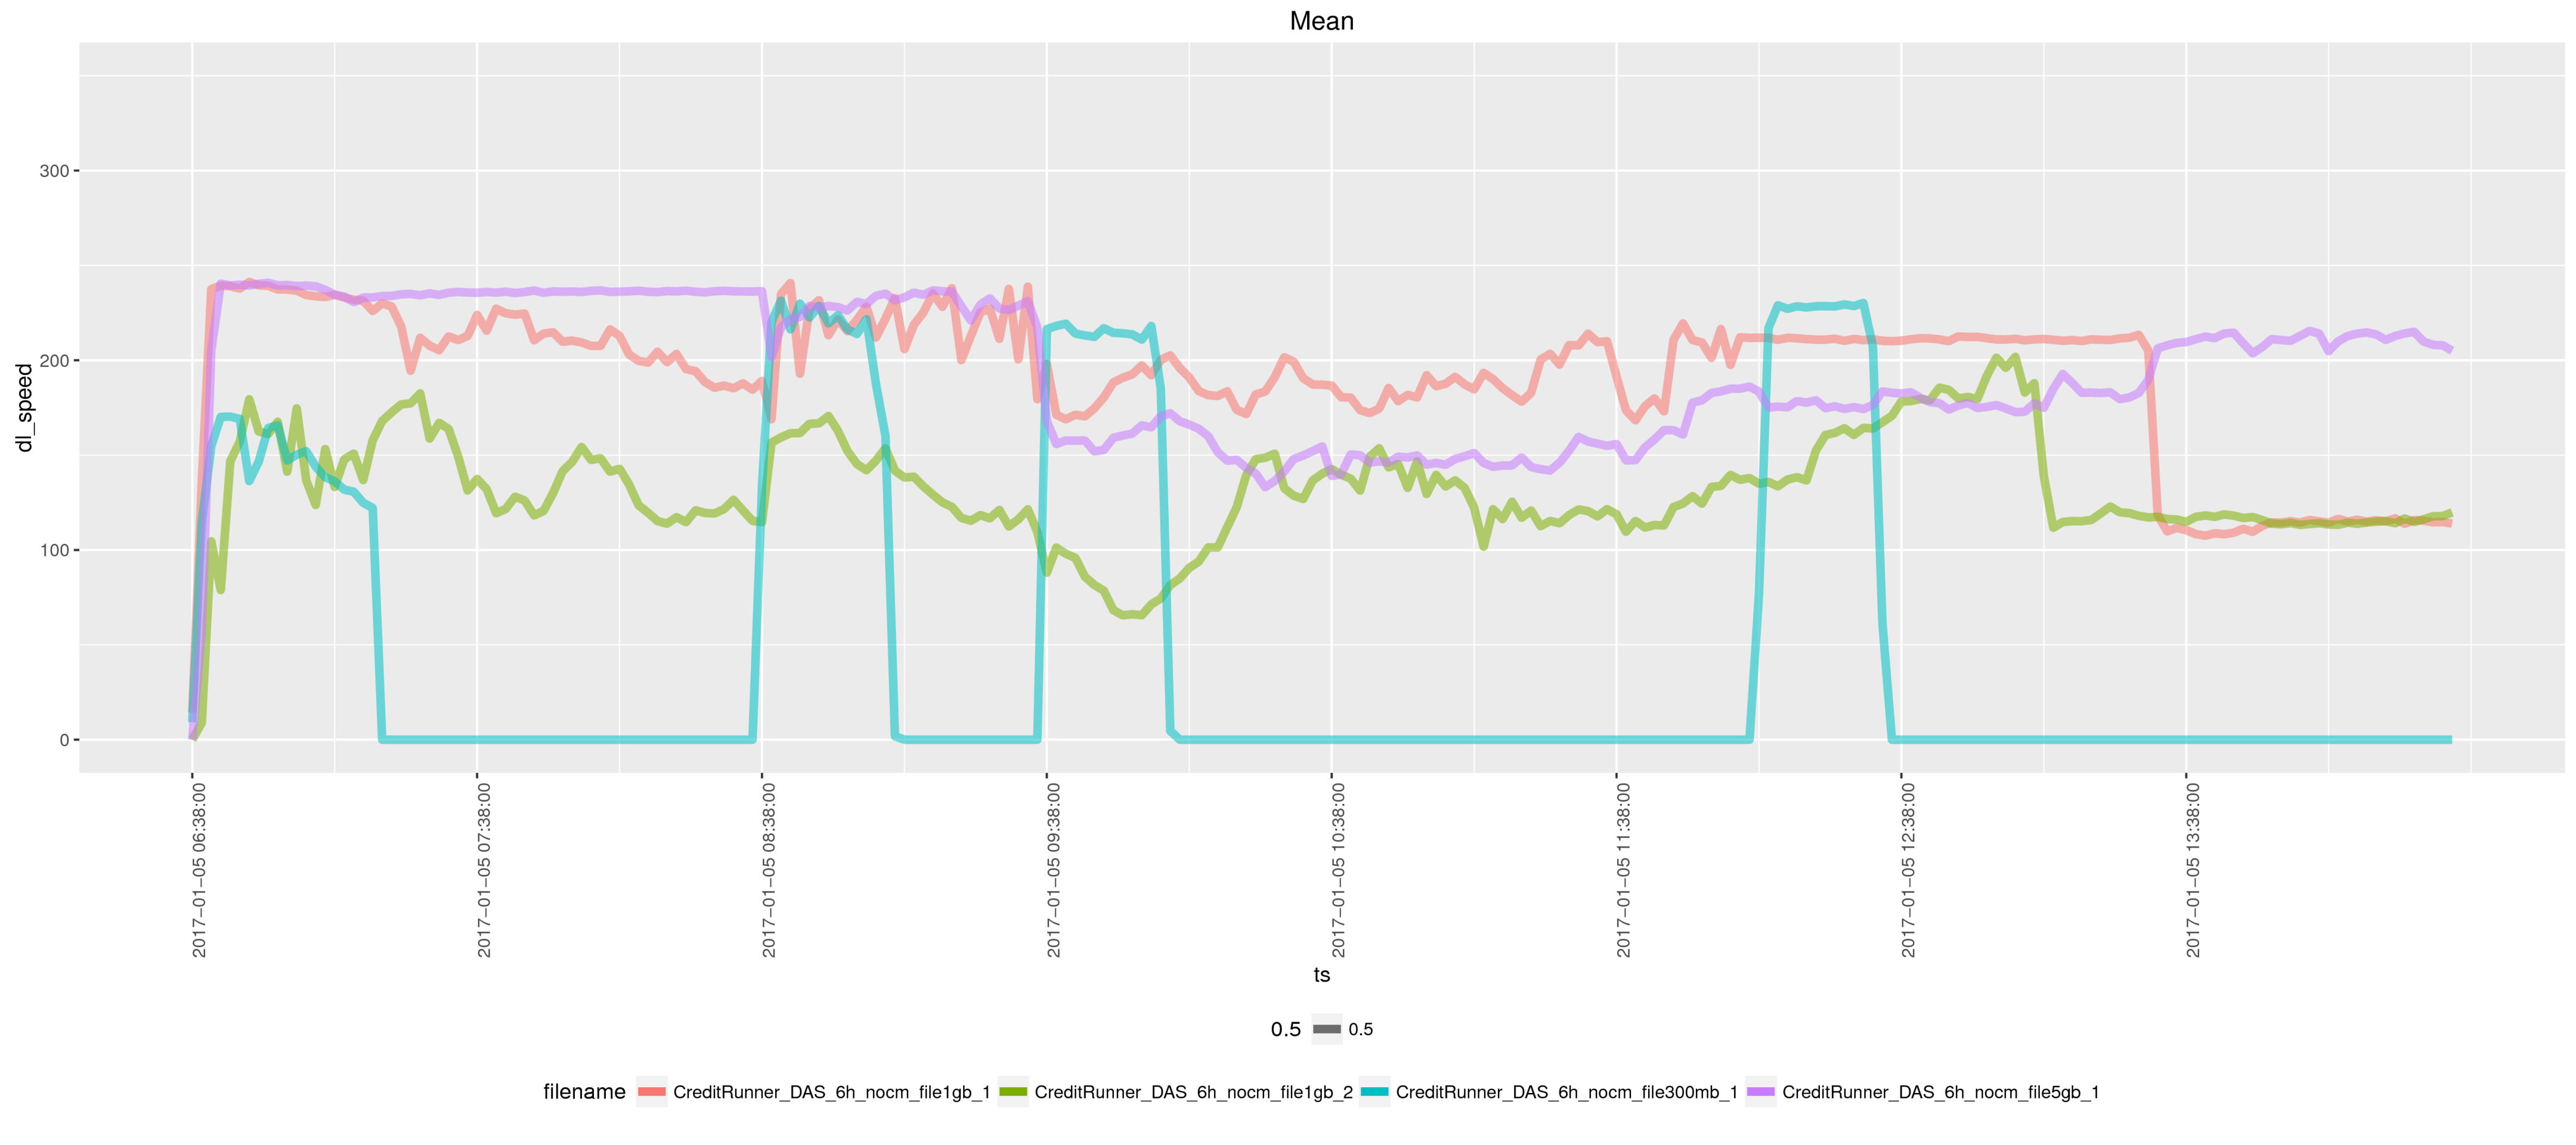
\includegraphics[width=\textwidth]{pics/results/reg_cma.png}
	\caption{Swarm performance with credit mining in the swarm}
	\label{fig:swarmcmperf}
\end{figure}

\begin{figure}[h]
	\centering
	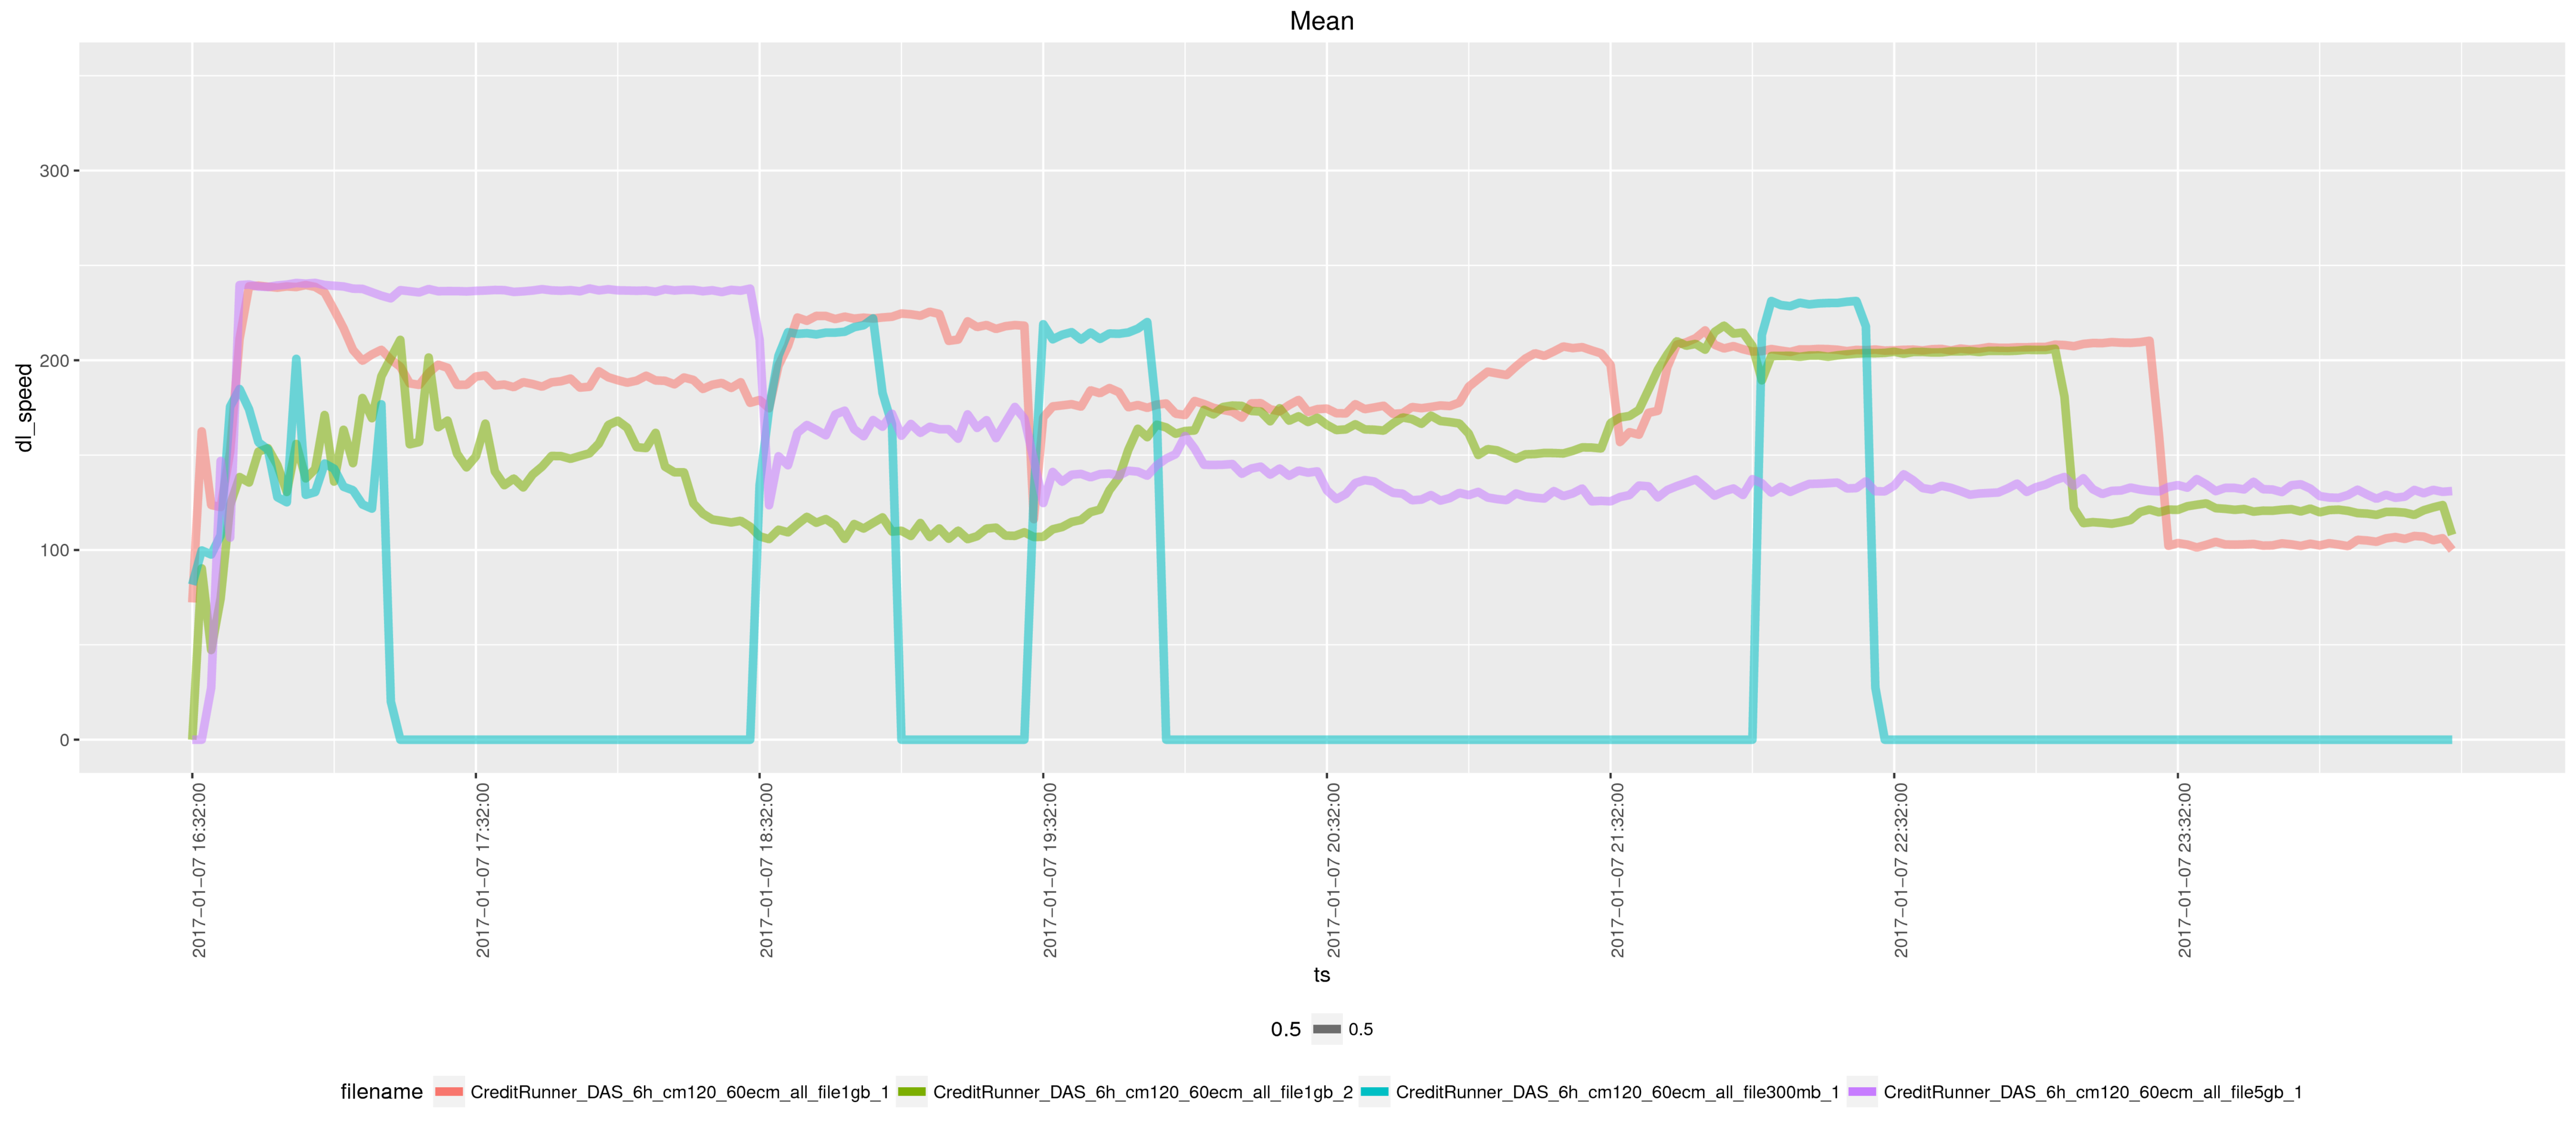
\includegraphics[width=\textwidth]{pics/results/reg_cm+60a.png}
	\caption{Swarm performance with credit mining outside the swarm (60 miners)}
	\label{fig:swarmcm60perf}
\end{figure}

\begin{figure}[h]
	\centering
	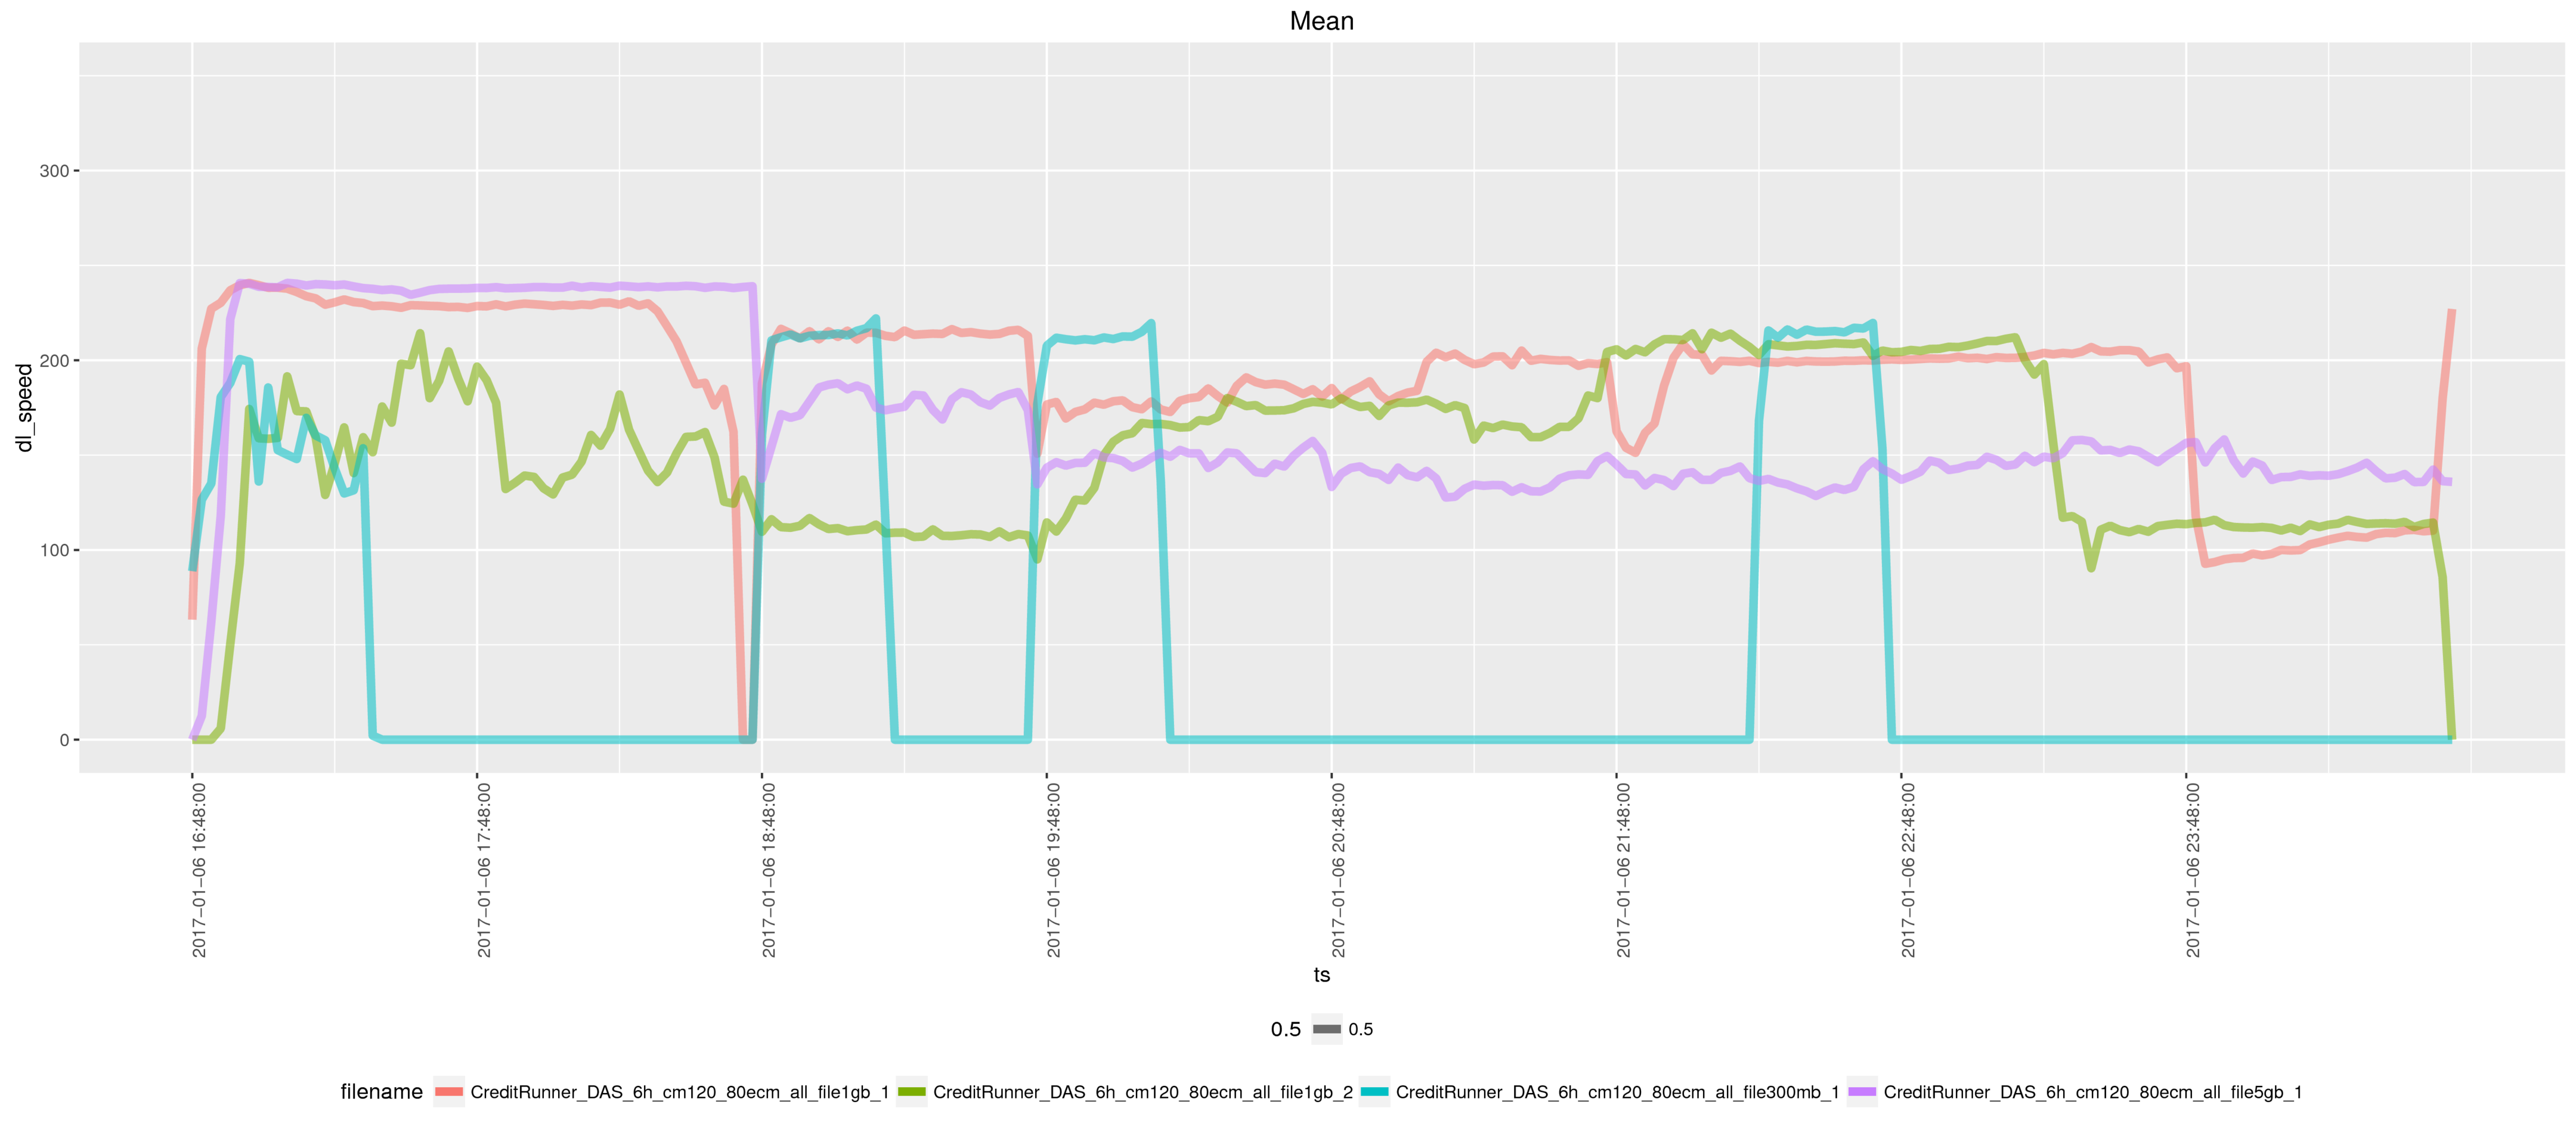
\includegraphics[width=\textwidth]{pics/results/reg_cm+80a.png}
	\caption{Swarm performance with credit mining outside the swarm (80 miners)}
	\label{fig:swarmcm80perf}
\end{figure}

\todo[inline]{single swarm}
\todo[inline]{scoring inside}

\clearpage
\section{Swarm choose}
\begin{table}[h]
	\centering
	\caption{Probability swarm chooser}
	\begin{adjustwidth}{-2.5cm}{}
		\begin{tabular}{|c|p{1.5cm}|p{1.5cm}|p{1.5cm}|p{1.5cm}||c|p{1.5cm}|p{1.5cm}|p{1.5cm}|p{1.5cm}|}
			\hline
			\rowcolor[HTML]{EFEFEF} 
			No. & \textit{sc} top 3 (top 6) & \textit{sr} top 3 (top 6) & \textit{sc} on top session & \textit{sr} on top session & No. & \textit{sc} top 3 (top 6) & \textit{sr} top 3 (top 6) & \textit{sc} on top session & \textit{sr} on top session \\ \hline
			1 & 0  (0) & 0  (0) & 0 & 0 & 19 & 1  (1) & 1  (1) & 1 & 2\\ \hline
			2 & 0  (0) & 1  (1) & 0 & 1 & 20 & 1  (1) & 1  (1) & 2 & 2\\ \hline
			3 & 0  (0) & 1  (1) & 0 & 1 & 21 & 1  (2) & 1  (1) & 2 & 2\\ \hline
			4 & 1  (2) & 1  (1) & 2 & 2 & 22 & 1  (2) & 1  (1) & 2 & 2\\ \hline
			5 & 1  (2) & 1  (1) & 2 & 1 & 23 & 1  (2) & 1  (1) & 2 & 2\\ \hline
			6 & 2  (3) & 1  (1) & 3 & 1 & 24 & 1  (1) & 1  (0) & 2 & 2\\ \hline
			7 & 2  (3) & 1  (1) & 3 & 1 & 25 & 1  (0) & 1  (0) & 2 & 2\\ \hline
			8 & 1  (2) & 1  (1) & 2 & 2 & 26 & 1  (0) & 1  (0) & 1 & 2\\ \hline
			9 & 2  (3) & 1  (1) & 3 & 1 & 27 & 1  (0) & 1  (0) & 1 & 1\\ \hline
			10 & 2  (3) & 1  (1) & 3 & 1 & 28 & 1  (0) & 1  (0) & 1 & 1\\ \hline
			11 & 2  (3) & 1  (1) & 3 & 1 & 29 & 1  (0) & 1  (0) & 1 & 1\\ \hline
			12 & 2  (3) & 1  (1) & 3 & 1 & 30 & 1  (0) & 1  (0) & 1 & 1\\ \hline
			13 & 2  (3) & 1  (1) & 3 & 1 & 31 & 1  (0) & 1  (0) & 1 & 1\\ \hline
			14 & 1  (2) & 1  (1) & 2 & 1 & 32 & 1  (0) & 1  (0) & 1 & 1\\ \hline
			15 & 1  (1) & 1  (1) & 2 & 2 & 33 & 0  (0) & 1  (0) & 0 & 1\\ \hline
			16 & 2  (2) & 1  (1) & 2 & 1 & 34 & 0  (0) & 1  (0) & 0 & 1\\ \hline
			17 & 1  (2) & 1  (1) & 2 & 1 & 35 & 0  (0) & 1  (0) & 0 & 1\\ \hline
			18 & 2  (1) & 1  (0) & 2 & 2 & 36 & 0  (0) & 0  (0) & 0 & 0\\ \hline
		\end{tabular}
	\end{adjustwidth}
\end{table}

Alternative : 

\begin{table}[h]
	\centering
	\caption{Probability swarm chooser (percentage)}
	\begin{adjustwidth}{-2.5cm}{}
		\begin{tabular}{|c|p{1.8cm}|p{1.8cm}|p{1.3cm}|p{1.3cm}||c|p{1.8cm}|p{1.8cm}|p{1.3cm}|p{1.3cm}|}
			\hline
			\rowcolor[HTML]{EFEFEF} 
			No. & \textit{sc} top 3 (top 6) & \textit{sr} top 3 (top 6) & \textit{sc} on top session & \textit{sr} on top session & No. & \textit{sc} top 3 (top 6) & \textit{sr} top 3 (top 6) & \textit{sc} on top session & \textit{sr} on top session \\ \hline
			1 & 0\%(0\%) & 0\%(0\%) & 0\% & 0\% & 19 & 33\%(33\%) & 33\%(33\%) & 33\% & 67\%\\\hline
			2 & 0\%(0\%) & 33\%(33\%) & 0\% & 33\% & 20 & 33\%(33\%) & 33\%(33\%) & 67\% & 67\%\\\hline
			3 & 0\%(0\%) & 33\%(33\%) & 0\% & 33\% & 21 & 33\%(67\%) & 33\%(33\%) & 67\% & 67\%\\\hline
			4 & 33\%(67\%) & 33\%(33\%) & 67\% & 67\% & 22 & 33\%(67\%) & 33\%(33\%) & 67\% & 67\%\\\hline
			5 & 33\%(67\%) & 33\%(33\%) & 67\% & 33\% & 23 & 33\%(67\%) & 33\%(33\%) & 67\% & 67\%\\\hline
			6 & 67\%(100\%) & 33\%(33\%) & 100\% & 33\% & 24 & 33\%(33\%) & 33\%(0\%) & 67\% & 67\%\\\hline
			7 & 67\%(100\%) & 33\%(33\%) & 100\% & 33\% & 25 & 33\%(0\%) & 33\%(0\%) & 67\% & 67\%\\\hline
			8 & 33\%(67\%) & 33\%(33\%) & 67\% & 67\% & 26 & 33\%(0\%) & 33\%(0\%) & 33\% & 67\%\\\hline
			9 & 67\%(100\%) & 33\%(33\%) & 100\% & 33\% & 27 & 33\%(0\%) & 33\%(0\%) & 33\% & 33\%\\\hline
			10 & 67\%(100\%) & 33\%(33\%) & 100\% & 33\% & 28 & 33\%(0\%) & 33\%(0\%) & 33\% & 33\%\\\hline
			11 & 67\%(100\%) & 33\%(33\%) & 100\% & 33\% & 29 & 33\%(0\%) & 33\%(0\%) & 33\% & 33\%\\\hline
			12 & 67\%(100\%) & 33\%(33\%) & 100\% & 33\% & 30 & 33\%(0\%) & 33\%(0\%) & 33\% & 33\%\\\hline
			13 & 67\%(100\%) & 33\%(33\%) & 100\% & 33\% & 31 & 33\%(0\%) & 33\%(0\%) & 33\% & 33\%\\\hline
			14 & 33\%(67\%) & 33\%(33\%) & 67\% & 33\% & 32 & 33\%(0\%) & 33\%(0\%) & 33\% & 33\%\\\hline
			15 & 33\%(33\%) & 33\%(33\%) & 67\% & 67\% & 33 & 0\%(0\%) & 33\%(0\%) & 0\% & 33\%\\\hline
			16 & 67\%(67\%) & 33\%(33\%) & 67\% & 33\% & 34 & 0\%(0\%) & 33\%(0\%) & 0\% & 33\%\\\hline
			17 & 33\%(67\%) & 33\%(33\%) & 67\% & 33\% & 35 & 0\%(0\%) & 33\%(0\%) & 0\% & 33\%\\\hline
			18 & 67\%(33\%) & 33\%(0\%) & 67\% & 67\% & 36 & 0\%(0\%) & 0\%(0\%) & 0\% & 0\%\\\hline
		\end{tabular}
	\end{adjustwidth}
\end{table}

Statistics (scoring vs seeder ratio): 
\begin{enumerate}
	\item Strictly larger Top 3  : 9 (25 \% better)
	\item Strictly larger Top 6  : 18 (50 \% better)
	\item Strictly larger top session  : 11
	\item larger or equal Top 3  : 32 (cover 88 \%)
	\item larger or equal Top 6  : 35 (cover 97 \%)
	\item larger or equal top session  : 30
\end{enumerate}

% CONCLUSIONS AND FUTURE WORK
\chapter{Conclusions and Future Work}
\label{chp:conclusionsandfuturework}

\section{Conclusions}
This thesis aims to solve the \bt~supply and demand misalignment introduced by freeriders. We devised an automatic mechanism to effectively gain credit in the existing credit system. We showed that it benefits both individuals and communities. The user can gain the credit without the need to seed for a long time. The swarms in the community can also get higher download speeds and content availability.

We then proposed the enhancement of \textit{credit mining system}, an autonomous system to download pieces from selected swarms in order to gain high upload ratio in the future. It can run on top of the traditional credit system that is already widely implemented in both private and public communities. The credit mining system finds swarms with high return potential, picks the rarest pieces, and uploads those to the community using all the available bandwidth.

We focused on the investment algorithm which is the core of credit mining. Two stages of the algorithm were presented. Both stages are important. The \textit{prospecting} stage filters a huge number of swarm while maintaining its resilience by not being solely dependent on a centralized tracker. The \textit{mining} stage only selects the best swarms, those that have a high gain potential. If necessary, it also stops problematic or low potential swarms. We also proposed the \textit{scoring} policy, a highly customizable method to quantify swarms into a score that can be compared with each other, which reduces any possible identical result.

The credit mining system is now fully integrated with Tribler. When enabled, it is tailored to not interfere with users' activity while downloading. Provided with an accessible GUI, a user can easily interact with the system to start investing. Before the system is implemented, it passed several tests and has proven to be stable across platforms. All the components designed so as to not hinder user experience while the credit mining system is active.

The performance of the credit mining system met our expectations. All the components were did their tasks properly. Prospecting is both fast and accurate to find and filter swarms on the Internet. The scoring policy successfully selects the most undersupplied swarms and surpasses previous policy accuracy. Moreover, it also stops both saturated and low potential swarms. With stimulating enabled, in most cases, the system use a large portion (80\%) of its resources. The upload/download ratio can reach up to 4.91 with an average of 3.71, although the target was only 2.0. After making the comparison, the current system can gain more credit than in prior work. We also showed that credit miners have a beneficial impact on the community as a whole. When the number of miners is half that of the peers, the credit miners can boost more than half of the swarms in a particular community by up to 29\%. Increasing the number of miners can increase the swarm coverage as well as the average peers' download speed.

\section{Future Work}
Currently, credit miners still see other miners as a normal peer. There might be a case in which a miner seeds to another miner, which is unnecessary. The key problem of "Co-Investors" is to recognize and utilize the existence of other miners. When recognizing other miners, investment can be more selective. There is less need to boost a swarm if there are already miners there, for example. 

Although we proposed the scoring policy in this thesis, the optimal \textit{multipliers} to reach the highest gain possible are still unknown. With many parameters, a study to find the weight and importance of those parameters is desired. Furthermore, this policy can be extended by adding more parameters while adopting the same calculation method.

Another aspect that still unknown is whether using different policies for different swarms is beneficial. Currently, the policy cannot be changed, and all of the swarms need to comply with a single policy. Moreover, as we have shown in the previous chapter, not all swarms are suitable for stimulation. The \textit{partial mining} mechanism is a method to apply different policies and optimizations to different swarm, in order to get the highest credit gain possible. 

% BIBLIOGRAPHY
%\bibliographystyle{bib/latex8}
\bibliographystyle{bib/IEEEtranN} % changed latex8, I think its compatible
\bibliography{bib/bibliography}

%\appendix

%\chapter{TODO APPENDIX NAME}
\label{app:}
Appendix body



\end{document}

